\documentclass[10pt,xcolor=dvipsnames,compress]{beamer}

\usepackage{pcelab_theme}
\usepackage{todonotes}
\usepackage{pcelab_style}
\usepackage{hyperref}
%\usepackage[algoruled,longend]{algorithm2e}
\usepackage{array}
\usepackage{graphicx}
\graphicspath{ {./images/} }
\usepackage{amsmath}
\newcolumntype{C}{>{\centering\arraybackslash} m{1.3in} }
\newcolumntype{M}{>{\centering\arraybackslash} m{1.in} }
\everymath{\displaystyle}
\long\def\/*#1*/{}

\beamertemplatenavigationsymbolsempty
%\usepackage[square,numbers]{natbib}
\usepackage{tcolorbox}
\usepackage{xcolor}
\usepackage[export]{adjustbox}
%===============================================================================
% 					  Presentation Title and Author  
%===============================================================================
\title[IMECE 2024]{
Chance constrained PDE-constrained optimal design strategies under\\high-dimensional uncertainty}
\subtitle{}

\author[Pratyush Kumar Singh]{Pratyush Kumar Singh and Danial Faghihi} 

\institute[UB]{\vspace{-0.2in}\\
Department of Mechanical and Aerospace Engineering\\University at Buffalo\vspace{0.05 in}\\
International Mechanical Engineering Congress Exposition\vspace{0.02in}\\
November 17 - November 21, 2024\\
Portland, OR\vspace{0.05in}\\
Data-Enabled Predictive Modeling, Scientific Machine Learning, and Uncertainty Quantification in Computational Mechanics \\
}

    \titlegraphic{\vspace{-0.4in}\\
\includegraphics[width=5cm]{PCE_logo1.png}}

\date[]{\vspace{-1.0 in}}
%===============================================================================
%===============================================================================



\begin{document}
%============================================================================================
%============================================================================================
%============================================================================================
\begin{frame}
\titlepage
\end{frame}
%==============================================
\begin{frame}{Motivation}
\small
\textbf{Silica Aerogel:} High-performance materials for next-generation building insulation. \\
\begin{figure}
    \centering
    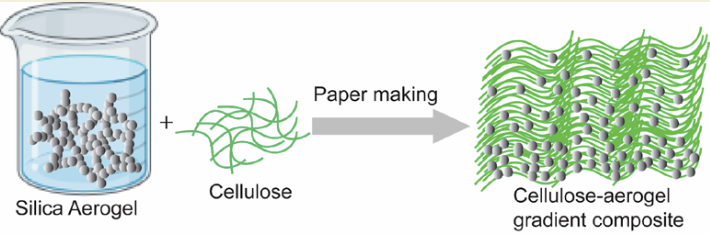
\includegraphics[width=0.4\textwidth]{Figures/aerogel_composite.png}~
    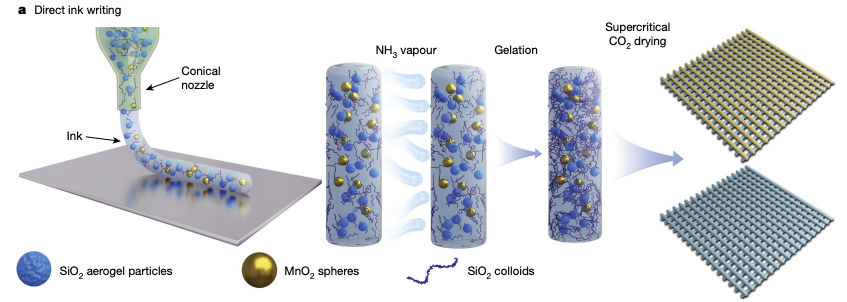
\includegraphics[width=0.5\linewidth]{Figures/Additive_manufacturing.png}\\
    \scriptsize{ Synthesis of aerogel-cellulose composite \footnotemark \hspace{0.2 in} Additive manufacturing  by direct ink writing \footnotemark}
    %\caption{Caption}
    \label{fig:additive}
\end{figure}
\textbf{Thermal breaks:} insulating components for \textbf{Net-Zero buildings}.\\
\begin{center}
    \hspace{0.0 in}
    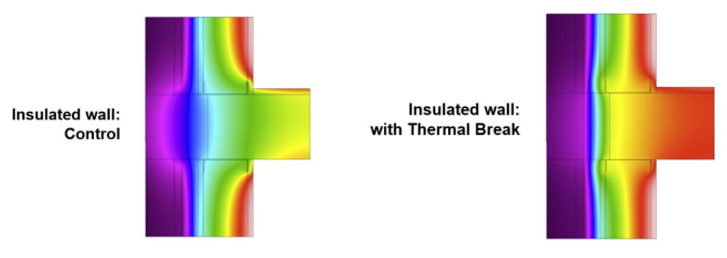
\includegraphics[width=0.4\textwidth]{Figures/Thermal_break_2.png} \\
    \scriptsize{ Effect of thermal break\footnotemark}
    \end{center}
\textbf{Design problem:} finding optimal spatial distribution of materials under uncertainty
    \footnotetext[1]{\scriptsize{Sarkar, {Singh}, Zhu, Faghihi, & Ren, 2024,  ACS Appl. Energy Mater}}
    \footnotetext[2]{\scriptsize{Zhao, Siqueira, Drdova, 2020, Nature .}}
    
    \footnotetext[3]{\scriptsize{Susorova et al., Buildings, 2016}}
\end{frame}
%===========================================================
\begin{frame}{Table of contents}
    \tableofcontents
\end{frame}

%=============================================


%============================================================================================
%============================================================================================
%============================================================================================
\section{Optimal Design under Uncertainty}
\begin{frame}{Outline}
    \tableofcontents[currentsection]
\end{frame}
\begin{frame}
\frametitle{Forward Model} 
\footnotesize
\textbf{Thermomechanical continuum model:}\\

\vspace{-0.1 in}
\begin{center}
    $\mathcal{R}(\boldsymbol{u},\red{\boldsymbol{\theta}},\blue{\boldsymbol{\zeta}}) = 0$
\end{center}
\vspace{-0.1in}
\begin{minipage}{0.46\textwidth} 
\footnotesize
\begin{center}
   Thermal Model 
\end{center}
\begin{equation*}
\boxed{
\begin{aligned}
\rho_s \textcolor{blue}{\phi_s} c_s \frac{\partial {\theta}_s}{\partial t} = \nabla \cdot ( \textcolor{blue}{\phi_s} \textcolor{red}{\kappa_s} \nabla {\theta}_s) - \textcolor{red}{h} ({\theta}_s - {\theta}_f) 
\\ 
\rho_f \textcolor{blue}{\phi_f} c_f \frac{\partial {\theta}_f}{\partial t} = \nabla \cdot ( \textcolor{blue}{\phi_f} \textcolor{red}{\kappa_f} \nabla {\theta}_f) + \textcolor{red}{h} ({\theta}_s - {\theta}_f)
\end{aligned}
}
\end{equation*}
\normalsize
\end{minipage}
\hfill
\begin{minipage}{0.46\textwidth} 
\footnotesize
\begin{center}
Mechanical Model  
\end{center}
\begin{equation*}
\boxed{
\begin{aligned}
\textcolor{red}{C} \frac{\partial p}{\partial t} + \frac{\partial }{\partial t}(\nabla \cdot \mathbf{u}_s) - \nabla \cdot \textcolor{red}{k} \nabla p &= 0
\\ 
\nabla \cdot \mathbf{T}_s (\mathbf{u}_s) &= 0 
\\
\mathrm{where,}\qquad\qquad\qquad\qquad\qquad
\\
\mathbf{T}_s = -\textcolor{blue}{\phi_s}\,p\mathbf{I} + \mathbf{T}^\prime_s    \qquad\,\,\,
            \\
             \mathbf{T}^\prime_s = 2\,\textcolor{red}{\mu}\,\mathbf{E}_s + \textcolor{red}{\lambda}\,\mathrm{tr}(\mathbf{E}_s)\mathbf{I}
\end{aligned}
}
\end{equation*}
\normalsize
\end{minipage}

\vfill


\small{
 States $\boldsymbol{u} = ( \theta_s, \theta_f, \boldsymbol{u_s}, p)$ $\xrightarrow[]{}$ solid/fluid temperature, solid displacement, fluid pressure \vspace{0.05in}\\
 Parameters \textcolor{red}{    $\boldsymbol{\theta} = (\kappa_s, \kappa_f, h, k, C, \mu, \lambda)$} $\xrightarrow[]{}$ determine from experimental data  \vspace{0.05in}\\ %(Bayesian inference)\\
  Design variables \textcolor{blue}{   $\boldsymbol{\zeta} = (\phi_s,\phi_f)$} $\xrightarrow[]{}$ determined to optimize component performance
\vspace{0.15 in}\\}
\textbf{Sources of uncertainty in $\blue{\boldsymbol{\zeta}}$:}
    \begin{itemize}
    \item Limited precision in manufacturing %: $\kappa = f(z+m)$
    \item Layer-by-layer deposition %(spatially correlated uncertainty)
    \end{itemize}
\vfill
\end{frame}
%============================================================================================
%============================================================================================
%============================================================================================

\begin{frame}{Design under Uncertainty}
\footnotesize
    \textbf{Spatially correlated uncertain parameter $m(\mathbf{x})$}
    \begin{itemize}
        \item Gaussian random fields $m \sim \mathcal{N}(\Bar{m},\mathcal{C})$
        \item Mat\'ern covariance kernel $\mathcal{C}=\mathcal{A}^{-2}$
        \begin{equation*}
        \mathcal{A} \, m = \begin{cases}
            \gamma \, \nabla \cdot( \boldsymbol{\Theta} \,\nabla m ) + \delta \, m  \quad\mathrm{in}\quad\Omega
                    \\
            (\boldsymbol{\Theta}\,\nabla m) \cdot \mathbf{n}  + \frac{\sqrt{\delta\,\gamma}}{1.42}\,m  \quad\mathrm{on}\quad\Gamma
        \end{cases}
    \end{equation*}
        \scriptsize
    \end{itemize}
    \begin{figure}[!htb]
\centering
\vspace{-0.05in}\\
\begin{tabular}{c c c c}
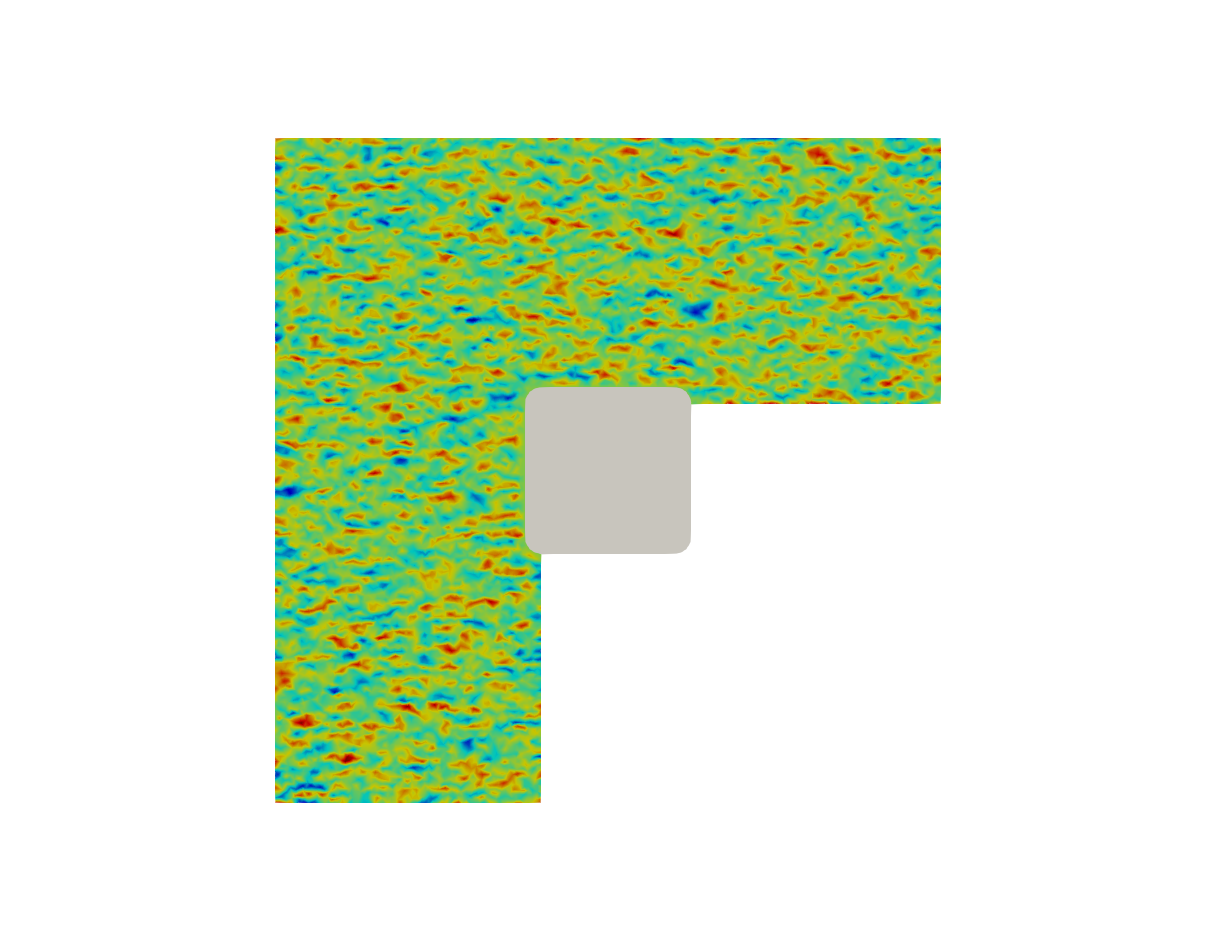
\includegraphics[trim={3.5in 2in 3.5in 2in},clip,width=0.16\textwidth]{Figures/low_1.png} &
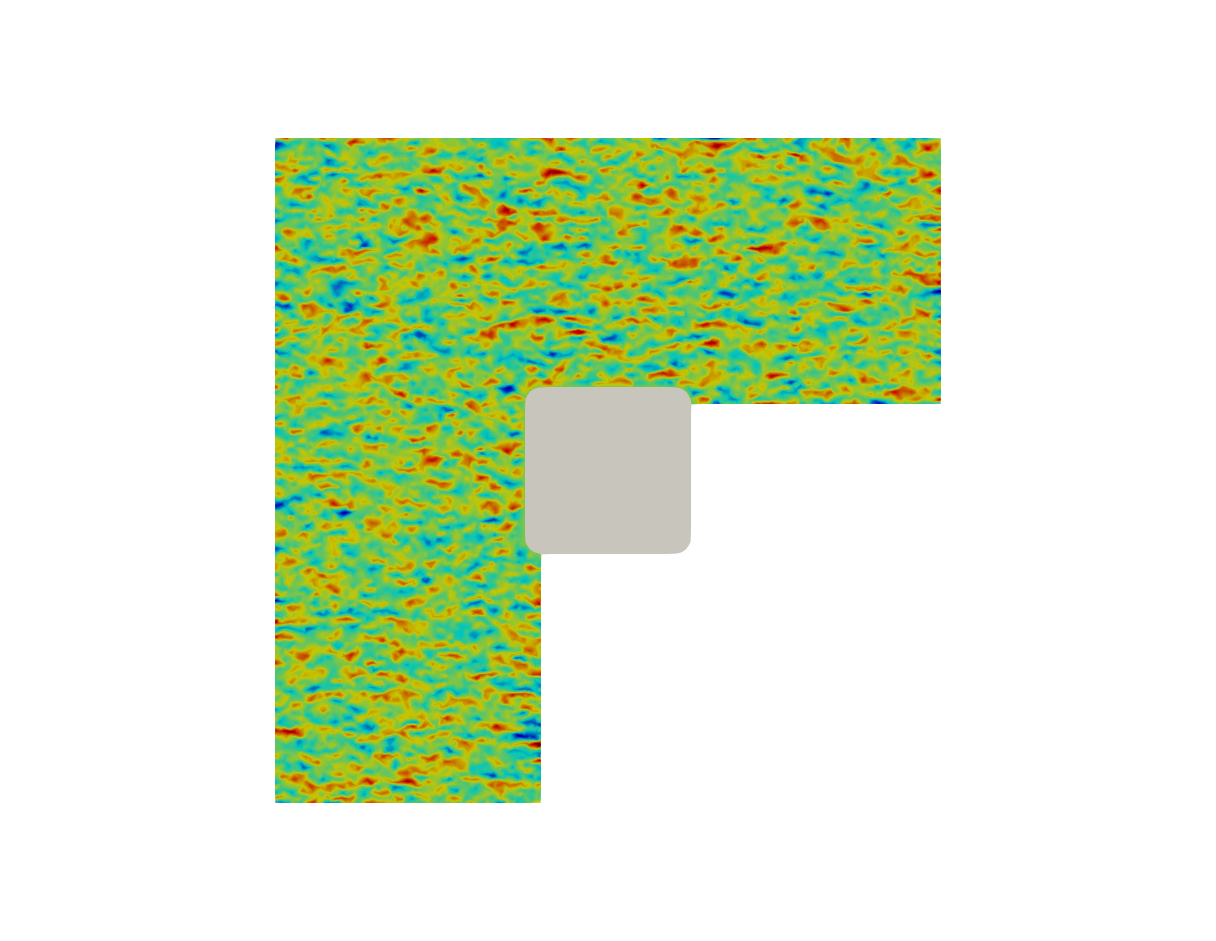
\includegraphics[trim={3.5in 2in 3.5in 2in},clip,width=0.16\textwidth]{Figures/low_2.png} &
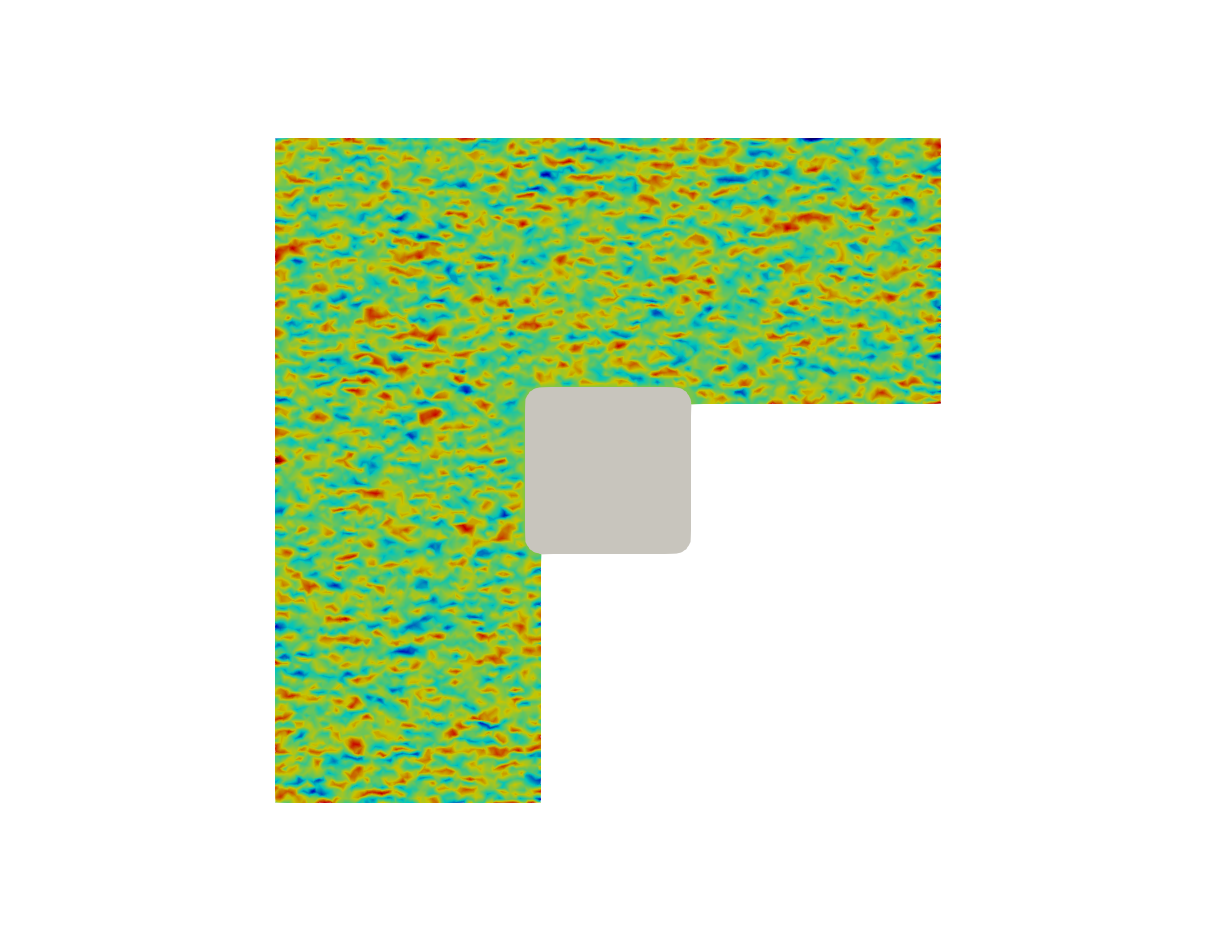
\includegraphics[trim={3.5in 2in 3.5in 2in},clip,width=0.16\textwidth]{Figures/low_3.png} &
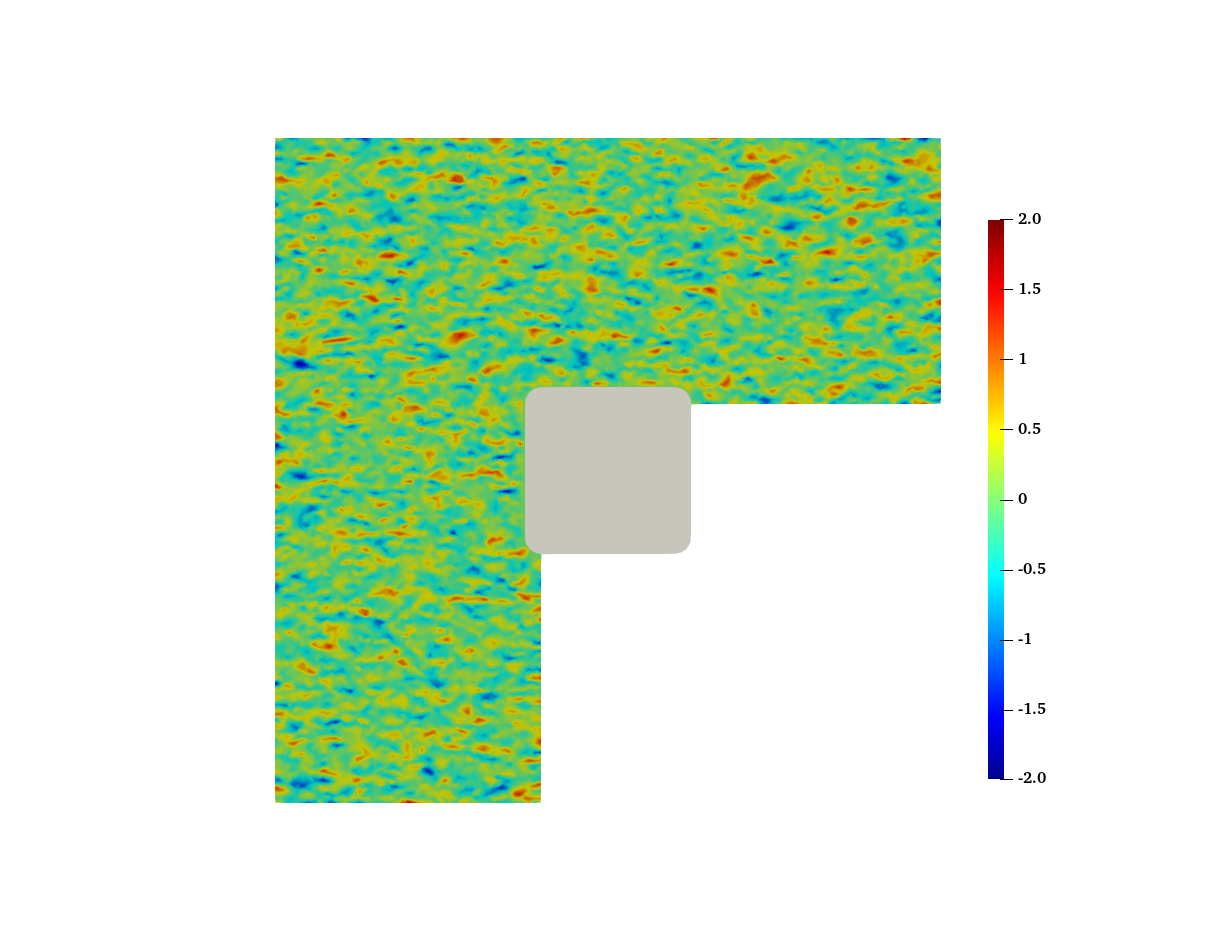
\includegraphics[trim={3.5in 2in 3.5in 2in},clip,width=0.16\textwidth]{Figures/low_4.png} 
 \end{tabular}
\\$L_c=0.02$\\
\begin{tabular}{c c c c}
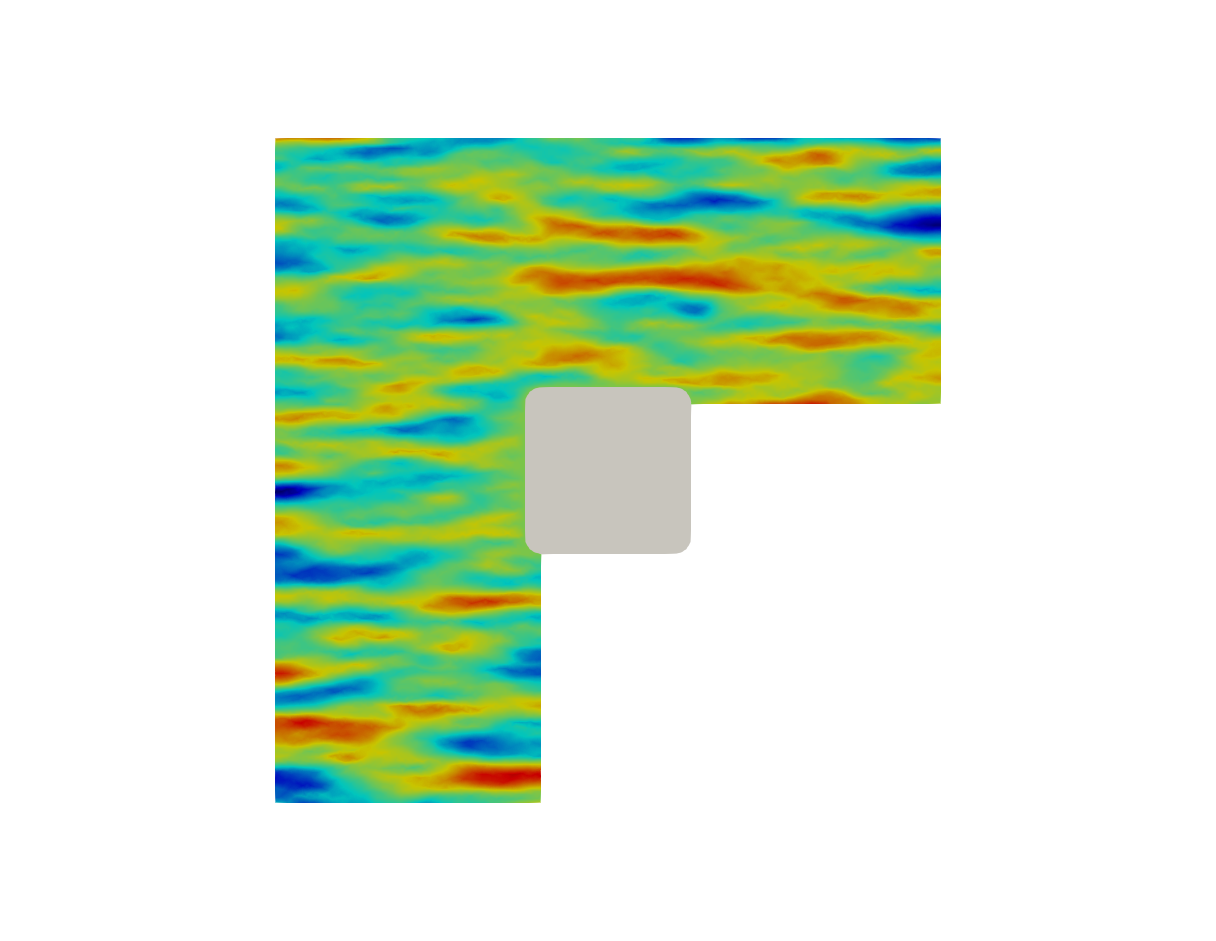
\includegraphics[trim={3.5in 2in 3.5in 2in},clip,width=0.16\textwidth]{Figures/high_1.png} &
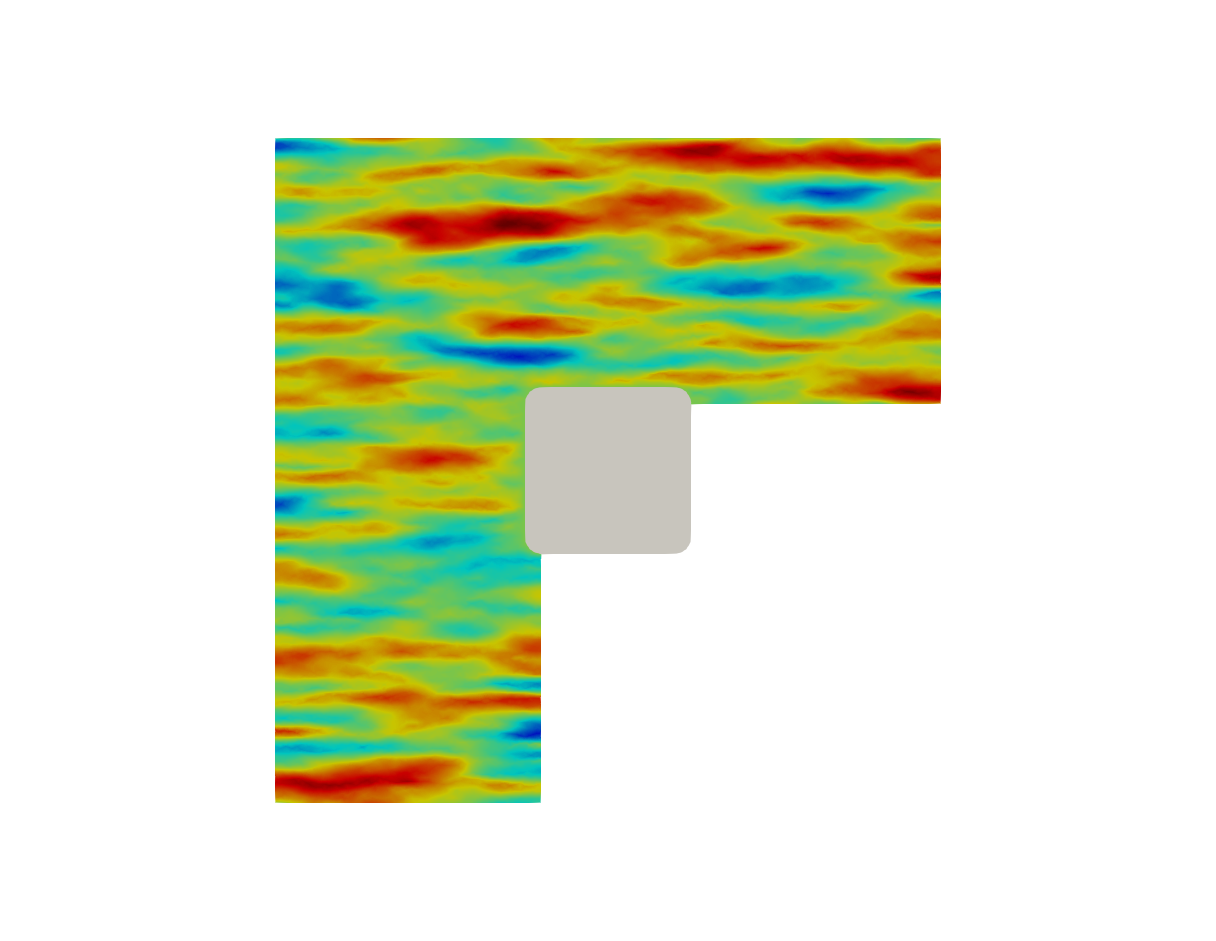
\includegraphics[trim={3.5in 2in 3.5in 2in},clip,width=0.16\textwidth]{Figures/high_2.png} &
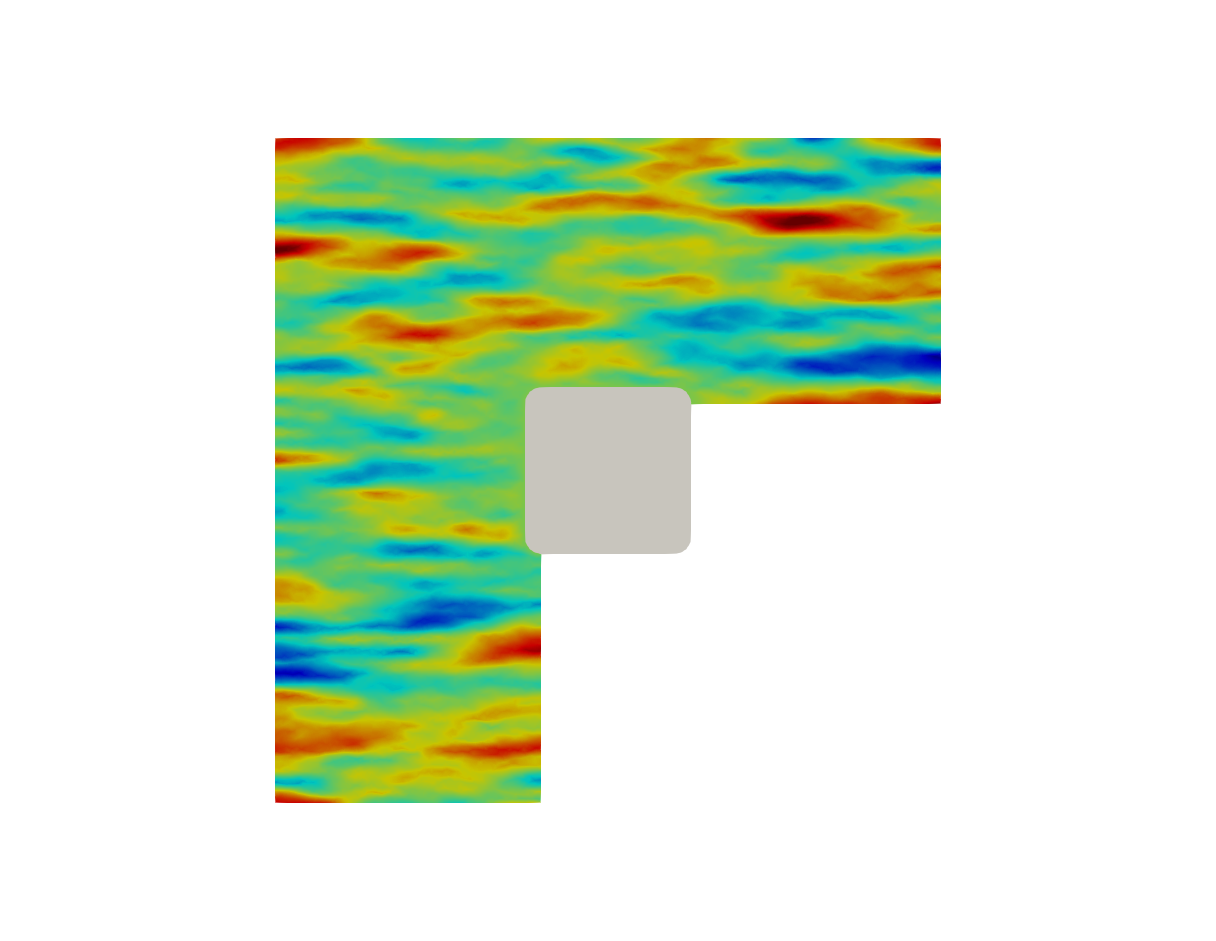
\includegraphics[trim={3.5in 2in 3.5in 2in},clip,width=0.16\textwidth]{Figures/high_3.png} &
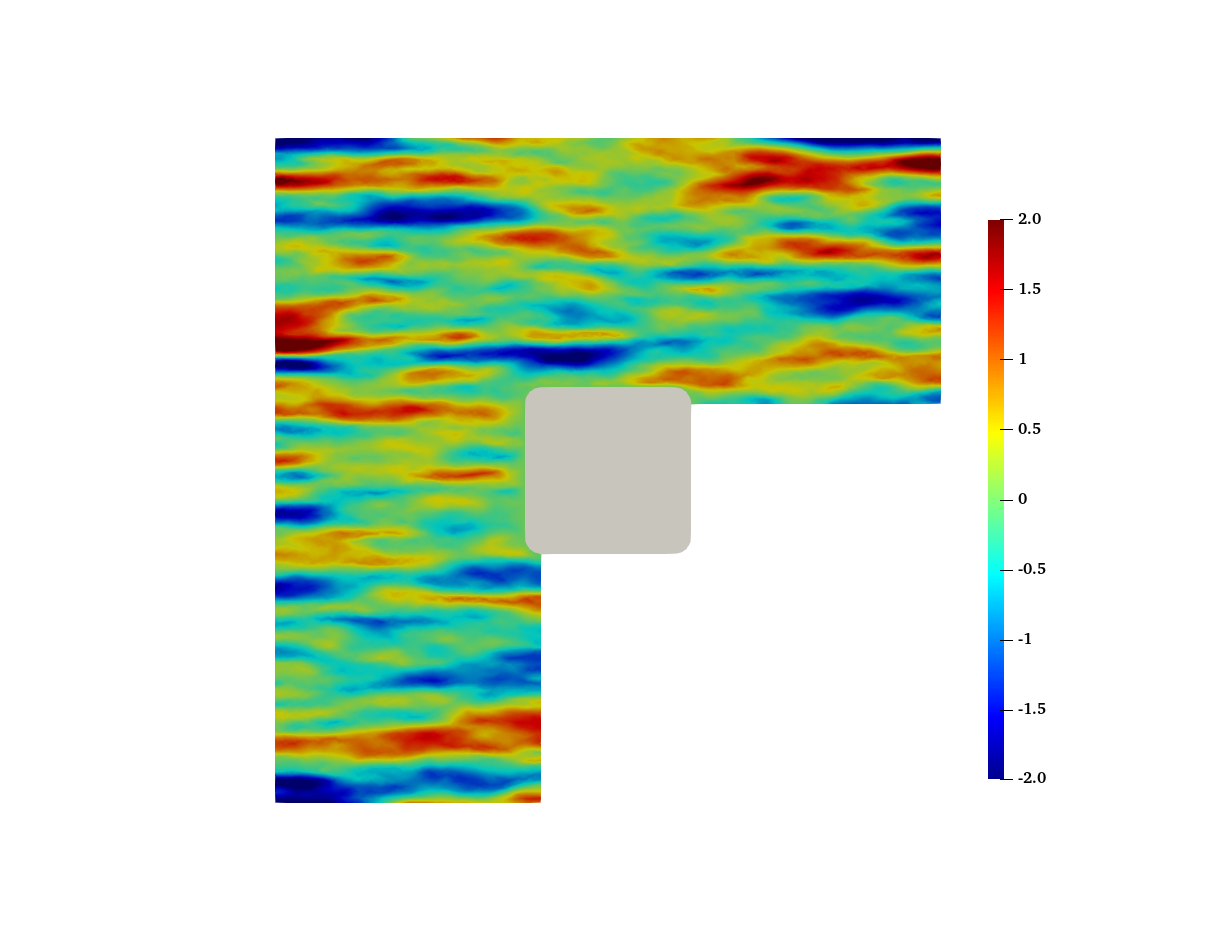
\includegraphics[trim={3.5in 2in 3.5in 2in},clip,width=0.16\textwidth]{Figures/high_4.png} 
\end{tabular}
\\$L_c=0.25$\vspace{-0.05in}\\
\end{figure}
\textbf{Design parameter $d(\mathbf{x})$}
\begin{itemize}
    %\item map between porosity $\phi_f \in [10 \%, 90 \%]$ and $d \in [0,1]$: 
    %\begin{equation*}
    %    \phi_f (\boldsymbol{x}) = \text{sigmoid}(d(\boldsymbol{x}) + m(\boldsymbol{x}))
    %\end{equation*}
    \item \textcolor{blue}{Blue}: $d=0 \xrightarrow{} \text{porosity} \: \phi_f = 90 \%$ weaker but more insulating aerogel
    \item \textcolor{red}{Red}: \:$d=1 \xrightarrow{} \text{porosity} \: \phi_f = 10 \%$ stronger but less insulating aerogel
\end{itemize}
\end{frame}
%============================================================================================
%============================================================================================
%============================================================================================
\begin{comment}
\begin{frame}{Design under Uncertainty}
    Determine spatial distribution of porosity with $10 \%$ and $90 \%$ porosity such that:
    \begin{itemize}
        \item avoid stress concentration
        \item maximizing thermal performance
    \end{itemize}
\textbf{Design objectives:}
\begin{itemize}
        \item Thermal Compliance:
        \begin{align*}
    \textcolor{red}{Q = -(\frac{1}{2} \sum_{i=s,f} {\langle \phi_i \kappa_i \nabla \theta_i,  \nabla \theta_i \rangle}_{\Omega}  + \sum_{i=s,f}  {\langle \phi_i h_{air} (\theta_i - \theta_{amb}), \theta_i \rangle }).}
\end{align*}
\end{itemize}

\textbf{Chance constraint:} Avoid stress concentration
    \begin{eqnarray*}
        \color{blue} {P(f(m,d)} \geq 0) &  = &  \mathbb{E}[\mathbb{I}_{[0,\infty]} (f(m,d))] \nonumber
        %& = & \int_{\mathcal{M}} \mathbb{I}_{[0,\infty]} (f(m,d)) \, d \mu(m),
    \end{eqnarray*} 
\[
 \color{blue} \mathbb{I}_{[0,\infty]} (f(m,d)) =
\begin{cases}
  \color{blue} 1 & \color{blue} \text{if } f(m,d) \geq 0 \\
  \color{blue} 0 & \color{blue} \text{if } f(m,d) < 0 \\
\end{cases}
\]
\begin{equation*}
    \textcolor{blue}{f = T_{cr} - max (T_{VM}(\boldsymbol{x})),}
\end{equation*}
$T_{cr}$ is the limiting critical stress and 
$(T_{VM}(\boldsymbol{x}))$ is the von Mises stress.
\end{frame}
\end{comment}
%============================================================================================
%============================================================================================
%============================================================================================
\begin{frame}{Design under Uncertainty}
\footnotesize
\begin{block}{\textbf{Risk-averse optimal design statement:}}
\centering
\begin{aligned}
     %& \hspace{-0.2 in}\text{\textbf{Risk-averse optimal design statement:}} \vspace{0.5in}\\
     \min_{{d}}  &\  \mathcal{J}({d})  =  \mathbb{E}[\textcolor{red}{Q({m},{d})}]  +  \beta_V\, \mathbb{V}[\textcolor{red}{Q({m},{d})}]  +  \beta_R\, R({d})
            \\
             \mathrm{s.t.\ } & \mathcal{R}(\boldsymbol{u},m,d) = 0 \\
             & P(\textcolor{blue}{f(m,d)} \geq 0) \leq \alpha_{c} \quad\mathrm{in\ }\Omega \\
           %\mathcal{V}^\prime
\end{aligned}
\end{block}
\textbf{Design objectives:} Thermal compliance 
\begin{itemize}
\begin{align*}
    \textcolor{red}{Q = -\bigg (\frac{1}{2} \sum_{i=s,f} {\langle \phi_i \kappa_i \nabla \theta_i,  \nabla \theta_i \rangle}_{\Omega}  + \sum_{i=s,f}  {\langle \phi_i h_{air} (\theta_i - \theta_{amb}), \theta_i \rangle } \bigg ).}
\end{align*}
\end{itemize}

\textbf{Chance constraint:} Avoid stress concentration
\begin{equation*}
    \textcolor{blue}{f} = T_{cr} - \blue{T_{\text{pn}}},
\end{equation*}
\textcolor{blue}{$T_{\text{pn}}$} is the p-norm of the Von Mises stress and $T_{cr}$ is the limiting critical stress.
\begin{equation*}
    \blue{T_{\text{pn}}} = {\left( \int_{\Omega} T_{\text{VM}}^{p} \,d \Omega \right)}^{\frac{1}{p}}
\end{equation*}
    \begin{eqnarray*}
        P(\textcolor{blue} {f(m,d)} \geq 0) &  = &  \mathbb{E}[\mathbb{I}_{[0,\infty]} \textcolor{blue}{(f(m,d))}] \nonumber
        %& = & \int_{\mathcal{M}} \mathbb{I}_{[0,\infty]} (f(m,d)) \, d \mu(m),
    \end{eqnarray*} 
\[
  \mathbb{I}_{[0,\infty]} \textcolor{blue}{(f(m,d))} =
\begin{cases}
   1 &  \text{if } \textcolor{blue}{f(m,d)} \geq 0 \\
   0 &  \text{if } \textcolor{blue}{f(m,d)} < 0 \\
\end{cases}
\]   
\end{frame}
%====================================================================
%====================================================================
%====================================================================
\begin{frame}{Design under Uncertainty}
\textbf{Computational Challenges}:
\begin{itemize}
    \item High-Dimensional parameter space $d(\boldsymbol{x}), m(\boldsymbol{x)}$\\
    \begin{center}
        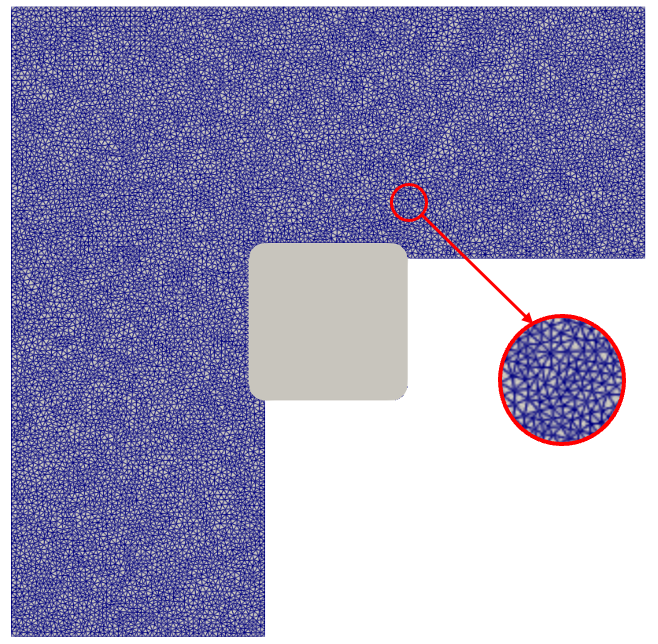
\includegraphics[width=0.22\textwidth]{Figures/mesh.png}\\
        \hspace{-0.1in}\footnotesize{27079 elements}\\
    \end{center}
               % \begin{itemize}
               % \item $\textcolor{blue}{d}(\mathbf{x}),\textcolor{red}{m}(\mathbf{x})$ are high-dimensional %fields 
               % (e.g.8587 nodes)
            %\end{itemize}
\end{itemize}
\hfill

\begin{itemize}
    \item Computing mean and variance of the design objective $Q$
            \begin{itemize}
                \item Monte Carlo approach, for $N$ samples, Convergence rate of $\mathcal{O}(\frac{1}{\sqrt{N}})$
                \scriptsize
                \begin{equation*}
                \mathbb{E}[Q] \approx \frac{1}{N}\sum_{i=1}^{N} Q(\textcolor{red}{m}^{(i)})
                ,
                \qquad
                \mathbb{V}[Q] \approx \bigg(\frac{1}{N}\sum_{i=1}^{N} Q^2(\textcolor{red}{m}^{(i)}) \bigg)   -   \bigg(  \frac{1}{N}\sum_{i=1}^{N} Q(\textcolor{red}{m}^{(i)})  \bigg)^2 
                \end{equation*}
            \end{itemize}
\end{itemize}
\begin{itemize}
    \item Chance constraint  
    \begin{itemize}
    \item Non-differentiability of the discontinuous indicator function.
        \item Approximation of constraint function requires large number of PDE solves.
    \end{itemize}
\end{itemize}

\end{frame}

%====================================================================
%====================================================================
%====================================================================
\section{Scalable Solution Algorithms}
\begin{frame}{Outline}
    \tableofcontents[currentsection]
\end{frame}

\begin{frame}{Scalable Algorithm: Taylor approximation}
\footnotesize


%\begin{center}
\begin{block}{\textbf{Risk-averse optimal design statement:}}
\centering
\begin{aligned}
     %& \hspace{-0.2 in}\text{\textbf{Risk-averse optimal design statement:}} \vspace{0.5in}\\
     \min_{{d}}  &\  \mathcal{J}({d})  =  \mathbb{E}[\textcolor{red}{Q({m},{d})}]  +  \beta_V\, \mathbb{V}[\textcolor{red}{Q({m},{d})}]  +  \beta_R\, R({d})
            \\
             \mathrm{s.t.\ } & \mathcal{R}(\boldsymbol{u},m,d) = 0 \\
             & P(\textcolor{blue}{f(m,d)} \geq 0) \leq \alpha_{c} \quad\mathrm{in\ } \Omega \\
           %\mathcal{V}^\prime
\end{aligned}
\end{block}
\vspace{0.05 in}\\
%\end{center}
\footnotesize
\textbf{Mean and Variance}
\begin{itemize}
    \item Taylor approximation of $Q$ at mean of
uncertain parameter $\overline{m}$ truncated with K terms
\begin{equation*}
    T_{K} Q(m,d) = \sum_{k=0}^K \partial_{m}^k Q(\overline{m},d) (m - \overline{m})^{k}
\end{equation*}
\item Quadratic $K=2$, with the objective, gradient and Hessian w.r.t. $m$ , evaluated at mean $\Bar{m}$, denoted as $\Bar{Q}$, $\Bar{Q}_m$ and $\Bar{Q}_{mm}$, and $<\cdot,\cdot>$ denotes the inner product

\begin{equation*}
                            T_2Q(m)  = \Bar{Q}  +   <\Bar{Q}_m, \,  m-\Bar{m}>  +  \frac{1}{2}<  \Bar{Q}_{mm}(m-\Bar{m}),  \,  m-\Bar{m}  >
\end{equation*}
\item Approximated mean and variance \footnotemark 
\begin{equation*}
     \mathbb{E}[T_2 Q] = Q(\overline{m},d) + \frac{1}{2} \textcolor{brown}{\mathrm{tr}(\mathcal{C}\,\Bar{Q}_{mm})}, \quad \mathbb{V}[T_2 Q] = <\Bar{Q}_m, \,    \mathcal{C}\,\Bar{Q}_m>  
                            + 
                            \frac{1}{2} \textcolor{brown}{\mathrm{tr}\bigg(       (\mathcal{C}\,\Bar{Q}_{mm})^2         \bigg)}
\end{equation*}
\end{itemize}
\scriptsize{\footnotetext[4]{Alexanderian, Petra, Stadler, Ghattas, 2017,SIAM Journal on Uncertainty Quantification}}
\end{frame}



%============================================================================================
%============================================================================================
%============================================================================================
\begin{frame}{Scalable Algorithm: Taylor approximation}
    \vfill
\textbf{Trace estimator}
\small 
\begin{itemize}


\item Generalize eigenvalues of $(\Bar{Q}_{mm},\mathcal{C}^{-1})$

        \begin{equation*}
            <\Bar{Q}_{mm}\,\psi_n,\,\phi>
            =
            \lambda_n
            <\mathcal{C}^{-1}\,\psi_n,\,\phi>  
            \qquad
            \forall\phi\in X,\, n\geq1
        \end{equation*}
        
        where $(\psi_n)_{n\geq1}\in X$ are the generalized eigenfunctions, $N_{eig}$ are number of dominant eigenvalues and $N_o$ is the oversampling factor. 
\end{itemize}

% \vspace{0.2in}
\vfill
\begin{itemize}
\item Randomized Singular Value Decomposition (SVD) algorithm 
    % \item Double pass randomized algorithm$^1$
\end{itemize}

\begin{minipage}{0.49\textwidth}
\begin{itemize}
    \item If eigenvalues decays rapidly, use $N_{eig}$ dominant eigenvalues \footnotemark
        
             $\mathrm{tr}\bigg(\mathcal{C}\,\Bar{Q}_{mm}\bigg)   \approx  \sum_{n\geq1}^{N_{eig}} \lambda_n$\\
            
             $\mathrm{tr}\bigg(       (\mathcal{C}\,\Bar{Q}_{mm})^2          \bigg) \approx \sum_{n\geq1}^{N_{eig}} \lambda_n^2$
        
        

\end{itemize}
\end{minipage}
\hfill
\begin{minipage}{0.5\textwidth}
\begin{figure}[H]
\centering
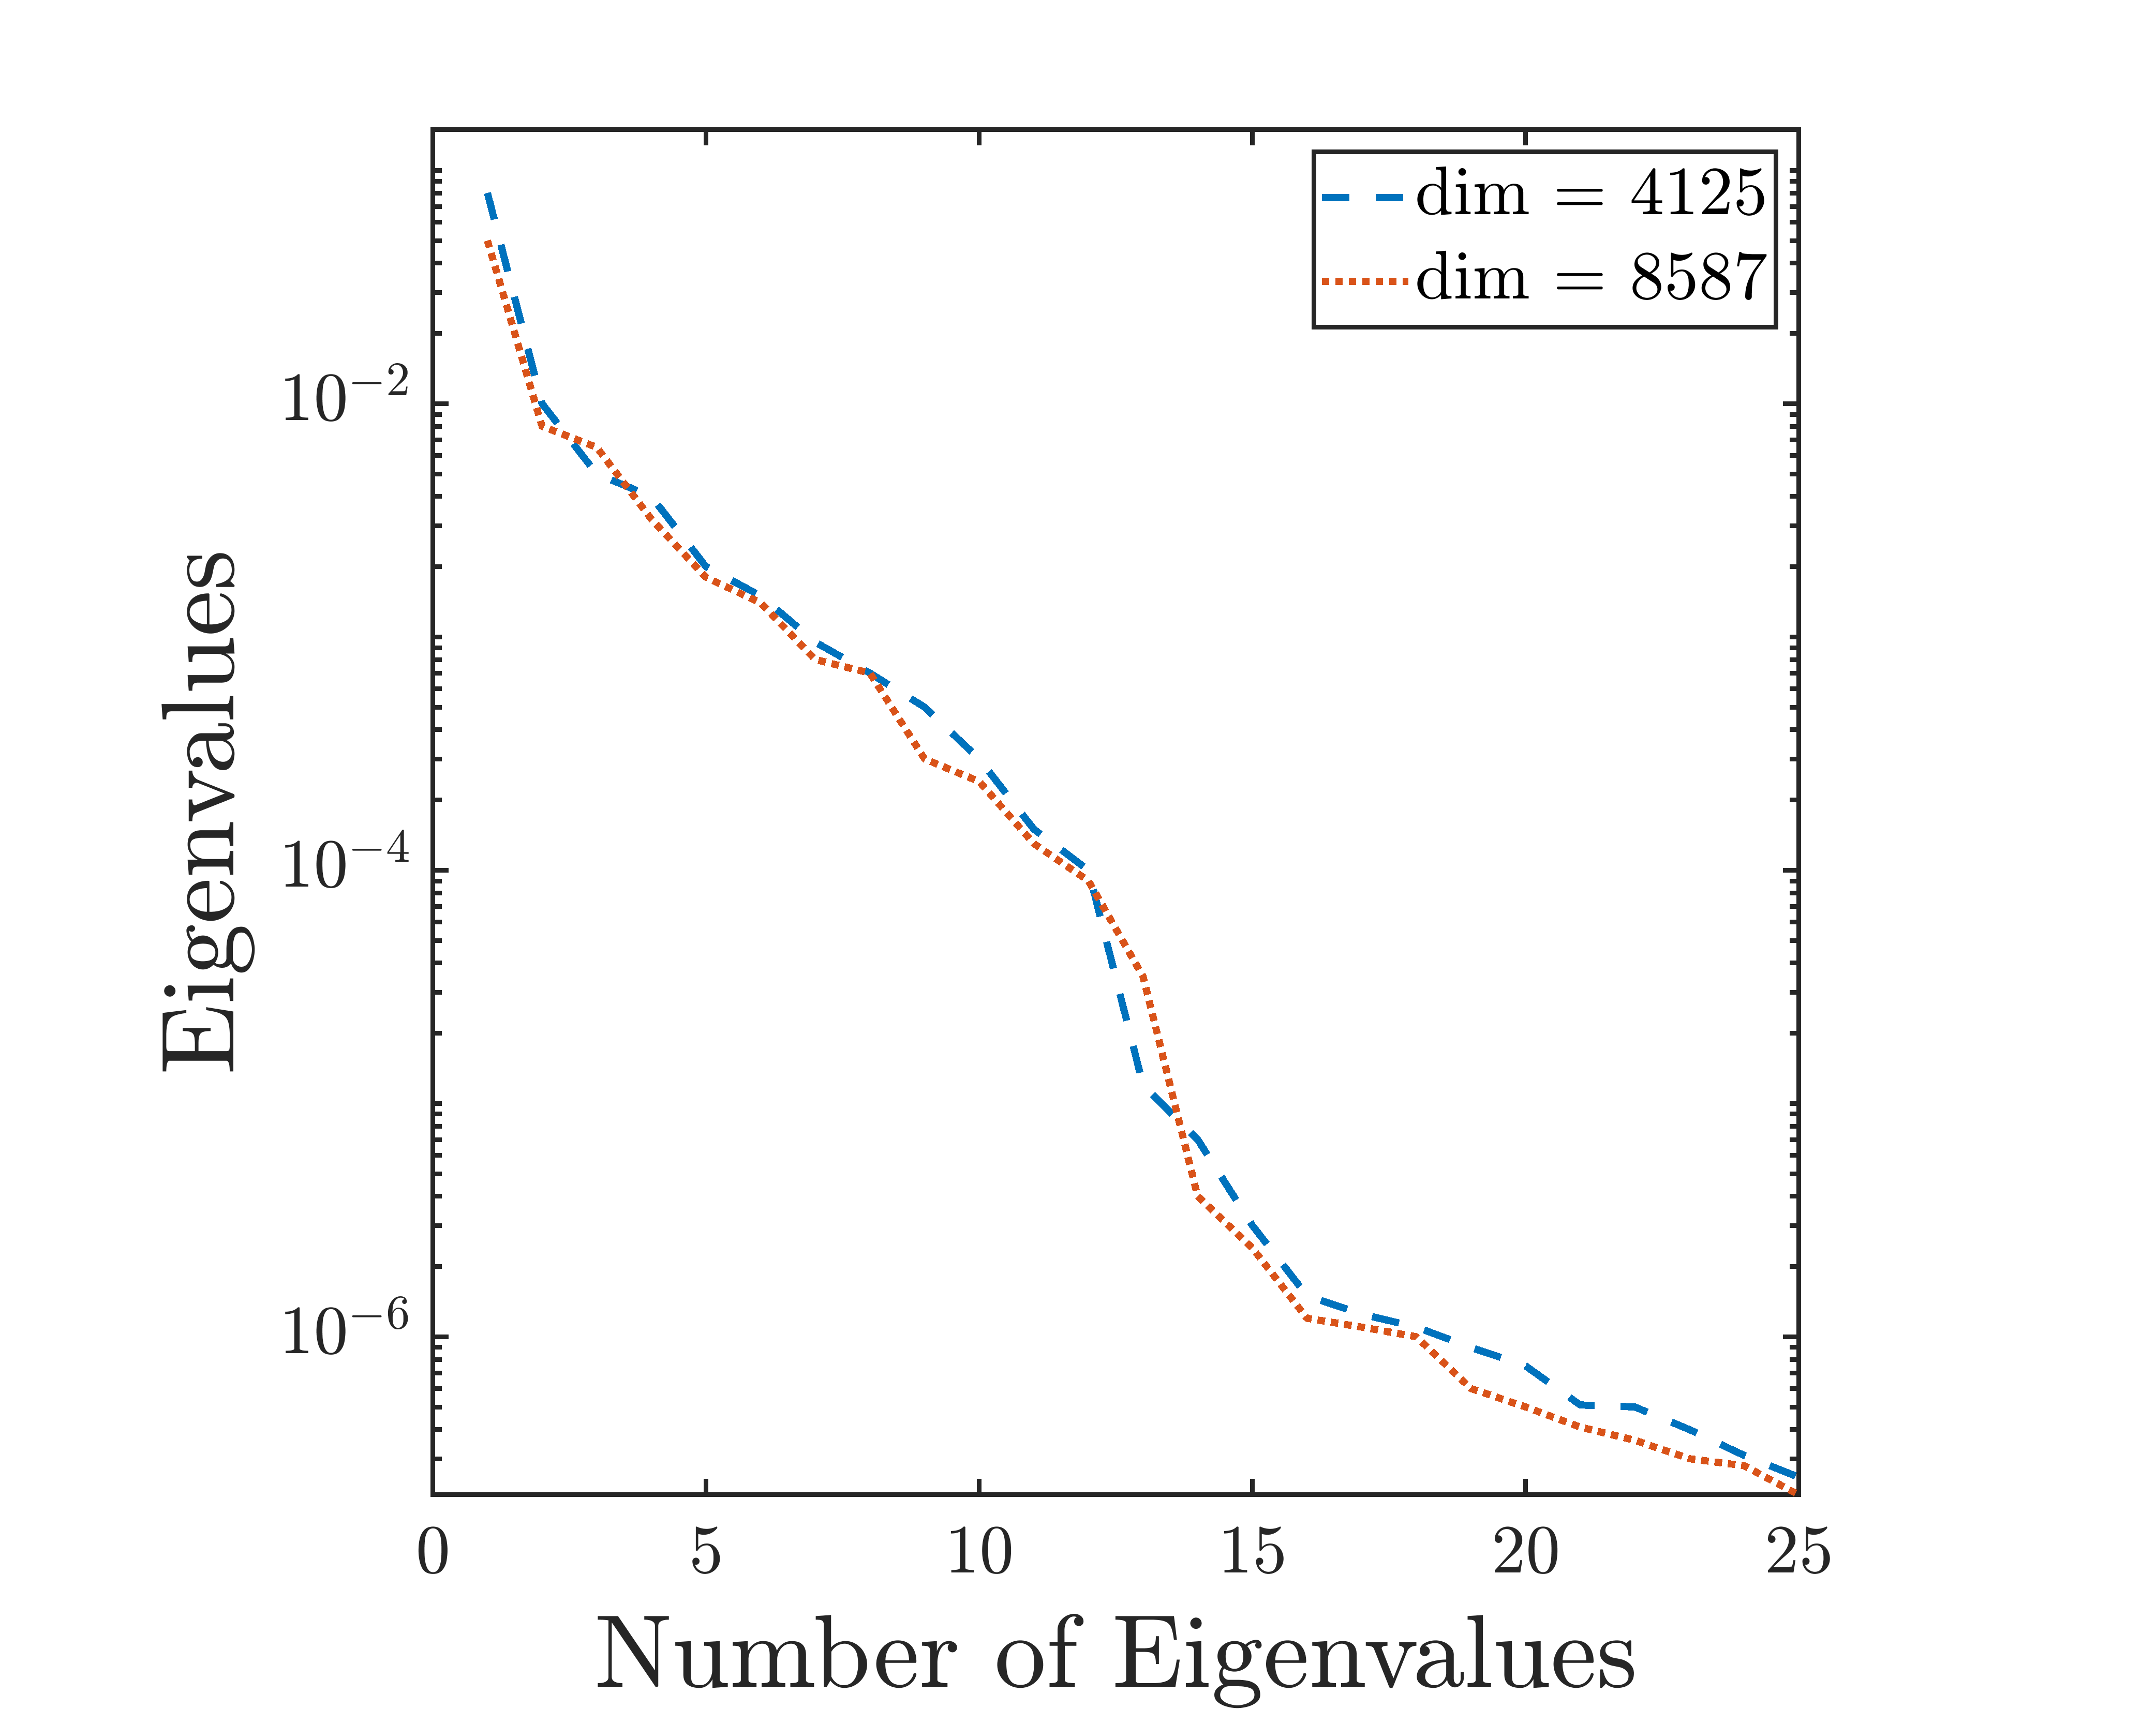
\includegraphics[trim = 0mm 0mm 0mm 0mm, clip,width=0.95\linewidth]{Figures/Eigenvalue_1.png}
\end{figure}
\end{minipage}

\vfill
\scriptsize
\footnotetext[5]{Peng, Villa, Ghattas, 2019, Journal of Computational Physics}

\end{frame}
%============================================================================================

%============================================================================================
%============================================================================================
\begin{frame}{Scalable Algorithm: Control Variate}
\footnotesize
\textbf{Mean correction:}\\
The Monte Carlo correction for the mean for Scalable Solution can be written as, 
\begin{align*}
    \mathbb{E}[Q]  = & \mathbb{E}[T_2 Q] + \mathbb{E}[Q - T_2 Q] \approx \textcolor{red}{\hat{Q}} := \overline{Q} + \frac{1}{2} tr(\mathcal{C}\,\Bar{Q}_{mm})\\
                       & + \frac{1}{M} \sum_{i=1}^{M}\left( Q(m_i) - \overline{Q} - <m_i - \overline{m}, \overline{Q}_m > - \frac{1}{2} <m_i - \overline{m}, \overline{Q}_{mm} (m_i - \overline{m})> \right).\\
\end{align*}
\textbf{Variance correction:}\\
The variance can be computed as,
\scriptsize{
\begin{align*}
       \hspace{-0.01in} \mathbb{V}[Q] = \mathbb{E}[{(T_2 Q - \overline{Q})}^2]+ \mathbb{E}[{(Q - \overline{Q})}^2-{(T_2 Q - \overline{Q})}^2]-{\left( \mathbb{E}[T_2 Q - \overline{Q}] + \mathbb{E}[(Q - \overline{Q})-(T_2 Q - \overline{Q})] \right)}^2
\end{align*}}
\footnotesize{The above expression for variance can be approximated as,}
\scriptsize{
\begin{align*}
        \textcolor{red}{\hat{{V}}}:= &< \mathcal{C} \overline{Q}_{m}, \overline{Q}_{m}> + \frac{1}{4}{(tr(\mathcal{C}\,\Bar{Q}_{mm}))}^2 + \frac{1}{2} tr({\mathcal{C}\,\Bar{Q}_{mm}}^2)\\
        & + \frac{1}{M}\sum_{i=1}^{M} \left( {(Q(m_i) - \overline{Q})}^2 - {\left(<m_i - \overline{m}, \overline{Q}_m> +\frac{1}{2} <m_i - \overline{m}, \overline{Q}_{mm} (m_i - \overline{m}> \right)}^2 \right) \\
        & - {\left( \frac{1}{2}tr(\mathcal{H}) + \frac{1}{M} \left( Q(m_i) -<m_i - \overline{m}>,\overline{Q}_m> - \frac{1}{2}<m_i - \overline{m},\overline{Q}_{mm} (m_i - \overline{m})> \right) \right)}^2
\end{align*}}
\end{frame}
%============================================================================================
%============================================================================================
%============================================================================================
\begin{frame}{ Scalable Algorithm}
\textbf{Chance constraint}
\begin{columns}
\begin{column}{0.45\textwidth}
\begin{itemize}
\small
%\item Approximation of constraint function requires large number of PDE solves.
\item \footnotesize{Scalable Solution of constraint at $\overline{m}$} %sample averaged approximation
\begin{equation*}
\footnotesize
    \hspace{-0.2in}P(\textcolor{blue}{f(m,d)})\geq 0) \approx \frac{1}{M_{f}} \mathbb{I}_{[0,\infty)}(T_{2}\textcolor{blue}{f(m_{i},d)}).
\end{equation*}
\item \footnotesize{Smooth approximation and quadratic penalty for chance constraint function\footnotemark}
\begin{equation*}
\footnotesize
    \mathbb{I}_{[0,\infty]}(x) \approx l_{\beta}(x) = \frac{1}{1 + e^{-2 \beta x}},  
\end{equation*}
\vspace{0.05in}
\begin{equation*}
    S_{\gamma}(x) = \frac{\gamma}{2}{(max{\{0,x\}})}^2
\end{equation*}
\vspace{0.05in}
\begin{equation*}
    \min_{{d}} \mathcal{J}_d + S_{\gamma}(x)(\mathbb{E}[l_{\beta}(\textcolor{blue}{f})] - \alpha_c)
\end{equation*}
\end{itemize}
\end{column}
\begin{column}{0.55\textwidth}
\centering
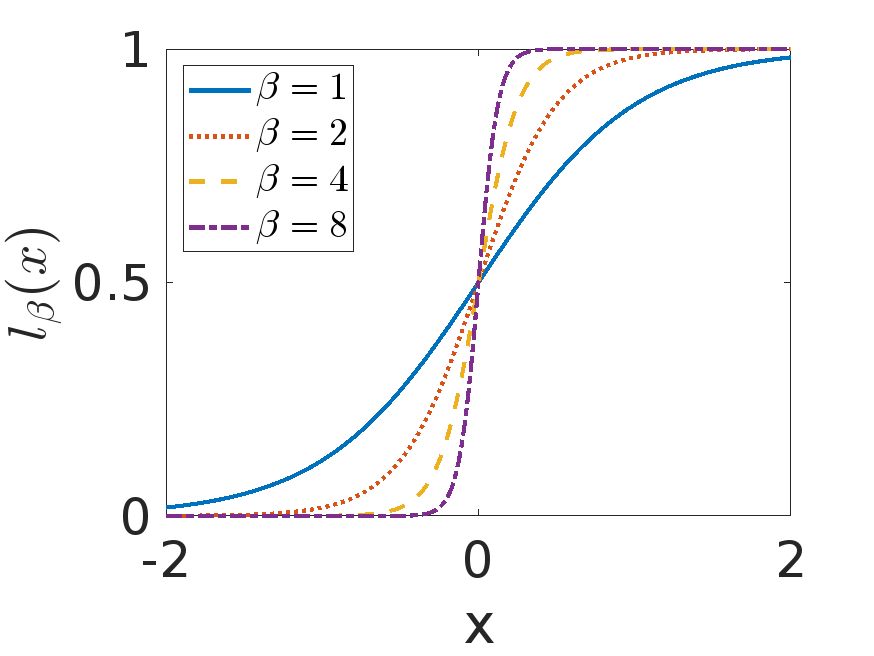
\includegraphics[trim={0.1in 0.1in 0.45in 0.2in},width=0.99\textwidth]{Figures/smooth.png}\\
\footnotesize{
\hspace{0.5 in}Smooth Approximation of\\\hspace{0.5in}Indicator Function}
\end{column}
\end{columns}

%\begin{center}
%    \hspace{2 in}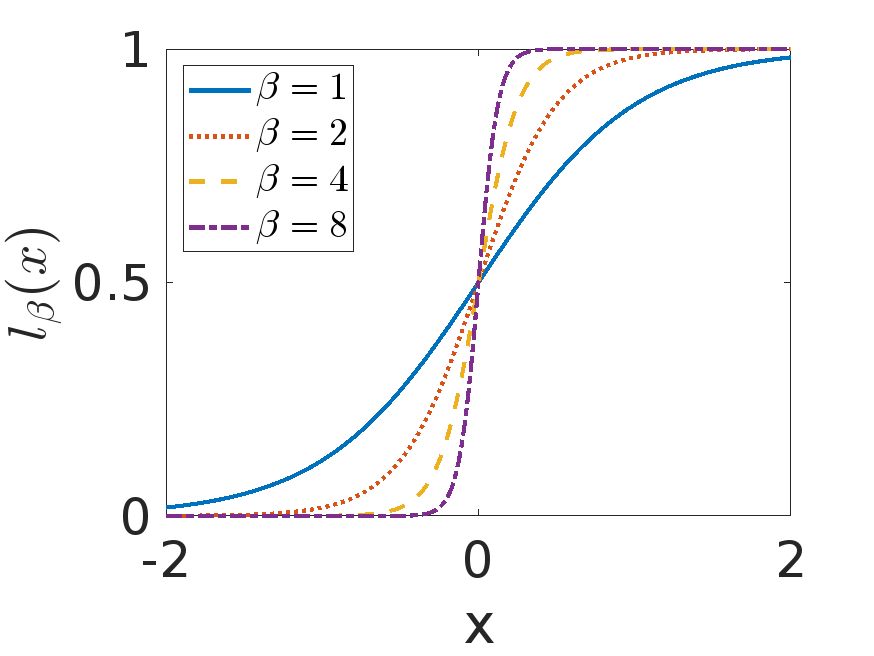
\includegraphics[width=0.45\textwidth]{Figures/smooth.png}
%\end{center}
\footnotetext[6]{Chen and Ghattas, 2021, SIAM Journal of Uncertainty Quantification}
\end{frame}
%============================================================================================
%============================================================================================
%============================================================================================


\begin{frame}
% \frametitle{Material design for target performance} 
\frametitle{Scalable Algorithm} 
\textbf{Lagrangian formulation}\\
\small
\vfill
% Gradient-Based Optimization via Adjoint
Analytical derivatives via Lagrange Formalism\vspace{0.05 in}\\
The weak form can be written as,
\begin{equation*}
    r(\mathbf{u},\mathbf{v},m,d) = {}_{\mathcal{V}} \langle \mathbf{v}, \mathcal{R}(\mathbf{u},m,d) \rangle {}_{\mathcal{V}^{'}}
\end{equation*}
\vfill
\begin{equation*}
    \mathcal{L}(\mathbf{u},\mathbf{v},m,d) = Q(\mathbf{u},m,d)+r(\mathbf{u},\mathbf{v},m,d),
\end{equation*}


\begin{table}[]
    \centering
    \begin{tabular}{c|c}
    \hline
      {State $\mathbf{u} = \{ \theta_s, \theta_f, \mathbf{u}_s, p  \}$}
      &   
      {Adjoint $\mathbf{v}$}  
      \\&
      \\\hline
      
      {$D_\mathbf{v}\mathcal{L}(\Bar{m}) = 0  $}  
      & 
      State problem  
      \\&$\langle  \Tilde{\mathbf{v}}, \partial_\mathbf{v}\Bar{r}  \rangle = 0$
      \\\hline
      
      {$D_\mathbf{u}\mathcal{L}(\Bar{m}) = 0  $}  
      & 
      Adjoint problem 
      \\&$\langle  \Tilde{\mathbf{u}}, \partial_\mathbf{u}\Bar{r}  \rangle = - \langle  \Tilde{\mathbf{u}}, \partial_\mathbf{u}\Bar{Q}  \rangle$
      \\\hline
      
        {$D_m\mathcal{L}(\Bar{m}) = 0  $} 
        &
      $m$-gradient  
      % \multicolumn{2}{c}{
      
      % }
      \\&$\langle  \Tilde{m}, \partial_m Q(\Bar{m})  \rangle = \langle  \Tilde{m}, \partial_m\Bar{r}  \rangle$
      \\\hline
 
      % \multicolumn{2}{c}{
      \blue{{$D_m f(\Bar{m}) = 0  $}}
        &
      \textcolor{blue}{{$m_f$-gradient}}  
      % \multicolumn{2}{c}{
      
      % }
      \\&$\langle  \Tilde{m}, \partial_m \textcolor{blue}{f(\Bar{m})}  \rangle = \langle  \Tilde{m}, \partial_m\Bar{r}  \rangle$
      \\\hline
      % }
    \end{tabular}
    % \caption{Caption}
    % \label{tab:my_label}
\end{table}

\vfill
\end{frame}
%============================================================================================
%============================================================================================
%============================================================================================

\begin{frame}
\frametitle{{Scalable Algorithm}} 
\vfill
\textbf{Lagrangian formulation}\\
\small
% Gradient-Based Optimization via Adjoint
Analytical derivatives via Lagrange Formalism
\vfill
\begin{equation*}
    \mathcal{L}^H (\mathbf{u},\mathbf{v},m,d; \hat{\mathbf{u}}, \hat{\mathbf{v}},\hat{m}) 
    =
    % \langle  \Tilde{m}, Q_m(\Bar{m})  \rangle
    % +
    \langle  \hat{m}, \partial_m\Bar{r}  \rangle
    +
    \langle  \hat{\mathbf{v}}, \partial_\mathbf{v}\Bar{r}  \rangle
    +
     \langle  \hat{\mathbf{u}}, \partial_\mathbf{u}\Bar{r}+\partial_\mathbf{u}\Bar{Q}  \rangle 
\end{equation*}


\begin{table}[]
    \centering
    \begin{tabular}{c|c}
    \hline
      State $\mathbf{u}$&  Incremental State $\hat{\mathbf{u}}$   
      \\
      Adjoint $\mathbf{v}$  &  Incremental Adjoint $\hat{\mathbf{v}}$   
      \\\hline
      {$D_\mathbf{v}\mathcal{L}^H(\Bar{m}) = 0  $ }
      &
      Incremental State problem 
       \\
      & 
      $\langle  \Tilde{\mathbf{v}}, \partial_{\mathbf{vu}}\Bar{r}\,\hat{\mathbf{u}}  \rangle 
    = - 
    \langle  \Tilde{\mathbf{v}}, \partial_{\mathbf{v}m}\Bar{r}\,\hat{m}  \rangle$  
      \\\hline
      {$D_\mathbf{u}\mathcal{L}^H(\Bar{m}) = 0  $  }
      &
      Incremental Adjoint problem
      \\
      & 
       $\langle  \Tilde{\mathbf{u}}, \partial_{\mathbf{uv}}\Bar{r}  \rangle 
    = - 
    \langle  
    \Tilde{\mathbf{u}}, \partial_{\mathbf{uu}}\Bar{r}\,\hat{\mathbf{u}}
    +
    \partial_{\mathbf{uu}} \Bar{Q}\,\hat{\mathbf{u}}
    +
    \partial_{\mathbf{u}m}\Bar{r}\,\hat{m}
    \rangle$
      \\\hline
      {$D_m\mathcal{L}^H(\Bar{m}) = 0  $}
    &
    $m$-Hessian
    \\
         &
    $\langle\Tilde{m}, \partial_{mm}Q(\Bar{m})\,\hat{m}\rangle 
       = 
      \langle \partial_{mm}\Bar{r}\,\hat{m}\rangle$
      \\
      &
      $\qquad+
      \langle  \Tilde{m}, \partial_{m\mathbf{v}}\Bar{r}\,\hat{\mathbf{v}}  \rangle +
      \langle \partial_{m\mathbf{u}}\Bar{r}\,\hat{\mathbf{u}} \rangle + \langle \partial_{mm}\Bar{Q}\,\hat{m} + \partial_{m\mathbf{u}}\Bar{Q}\,\hat{\mathbf{u}} \rangle$
      \\\hline
      \textcolor{blue}{{$D_m f(\Bar{m}) = 0  $}}
     %------------------------m_f Hessian-----------------------
    &
    \textcolor{blue}{$m_f$-Hessian}
    \\
         &
    $\langle\Tilde{m}, \partial_{mm}\textcolor{blue}{f(\Bar{m})}\,\hat{m}^{f}\rangle 
       = 
      \langle \partial_{mm}\Bar{r}\,\hat{m}^{f}\rangle$
      \\
      &
      $\qquad+
      \langle  \Tilde{m}, \partial_{m\mathbf{v}}\Bar{r}\,\hat{\mathbf{v}}^{f}  \rangle +
      \langle \partial_{m\mathbf{u}}\Bar{r}\,\hat{\mathbf{u}}^{f} \rangle + \langle \partial_{mm}\textcolor{blue}{{f}(\Bar{m})}\,\hat{m} + \partial_{m\mathbf{u}}\Bar{f}\,\hat{\mathbf{u}}^{f} \rangle$
    

      \\\hline
    \end{tabular}
\end{table}




\vfill
\end{frame}
%============================================================================================
%============================================================================================
%============================================================================================
\begin{frame}
% \frametitle{Material design for target performance} 
\frametitle{Scalable Algorithm} 
%\textbf{Lagrangian formulation}\\
\footnotesize
\vfill





\begin{alertblock}{Quadratically Approximated Cost Function}
    \begin{equation*}
    \min_{{d}} \: \mathcal{J}_\mathrm{quad}(d)
    =
    \bigg(
    \Bar{Q} + \frac{1}{2}
            \sum_{j\geq1}^{N_\mathrm{eig}}  \lambda_j
    \bigg)
    +
    \beta_V
    \bigg(
    \big<  \Bar{Q}_m, \mathcal{C}\,\Bar{Q}_m \big> 
    +
    \frac{1}{2}
    \sum_{j\geq1}^{N_\mathrm{eig}}  \lambda_j^2
    \bigg)
    +
    \beta_R \, R(d)
\end{equation*}
\begin{equation*}
    \hspace{-1.8 in} \text{s.t.} \frac{1}{M_f} \sum_{i=1}^{M_f} \mathbb{I}_{[0,\infty)]} (T_2 \textcolor{blue}{f(m_i,d)}) \leq \alpha_c \quad \text{in} \: \Omega
\end{equation*}
\end{alertblock}
\vspace{0.05in}\\
\begin{alertblock}{Quadratically Approximation as Control Variate}
    \begin{equation*}
      \hspace{-2 in} \min_{{d}} \:  \mathcal{J}_{\mathrm{quad}}^{CV}(d) = \hat{Q} + \beta_V \hat{V} + \beta_R R(d)
    \end{equation*}
    \begin{equation*}
         \hspace{-1.7 in} \text{s.t.} \frac{1}{M_f} \sum_{i=1}^{M_f} \mathbb{I}_{[0,\infty)]} (T_2 \textcolor{blue}{f(m_i,d)}) \leq \alpha_c \quad \text{in} \: \Omega
    \end{equation*}
    \begin{equation*}
         \hspace{-2.35 in} \text{Mean:}   \qquad \hat{Q} \approx \mathbb{E}[T_2 Q] + \mathbb{E}[Q - T_2 Q]
    \end{equation*}
    \begin{equation*}
         \hspace{-1.45 in} \text{Variance:} \quad \hat{V} \approx \mathbb{E}[{(T_2 Q - Q(\Bar{m}))}^2] - {(\mathbb{E}[T_2 Q - Q(\Bar{m})])}^2
    \end{equation*}
\end{alertblock}
Newton Conjugate Gradient is used as optimizer through computation of design gradients.
\vfill
\end{frame}
%============================================================================================
%============================================================================================
%============================================================================================






\section{Numerical Results}
\begin{frame}{Outline}
    \tableofcontents[currentsection]
\end{frame}

%================================================================================
%================================================================================
%================================================================================
\begin{frame}{Results: Beam-Insulator System}
%\begin{block}{\textbf{Risk-averse optimal design statement:}}
\centering
%\begin{aligned}
     %& \hspace{-0.2 in}\text{\textbf{Risk-averse optimal design statement:}} \vspace{0.5in}\\
%     \min_{{d}}  &\  \mathcal{J}({d})  =  \mathbb{E}[\textcolor{red}{Q({m},{d})}]  +  \beta_V\, \mathbb{V}[\textcolor{red}{Q({m},{d})}]  +  \beta_R\, R({d})
%            \\
%             \mathrm{s.t.\ } & \mathcal{R}(\boldsymbol{u},m,d) = 0 \\
%             & P(\textcolor{blue}{f(m,d)} \geq 0) \leq \alpha_{c} \quad\mathrm{in\ } \Omega \\
           %\mathcal{V}^\prime
%\end{aligned}
%\end{block}
%\vspace{0.05 in}\\
\begin{center}
    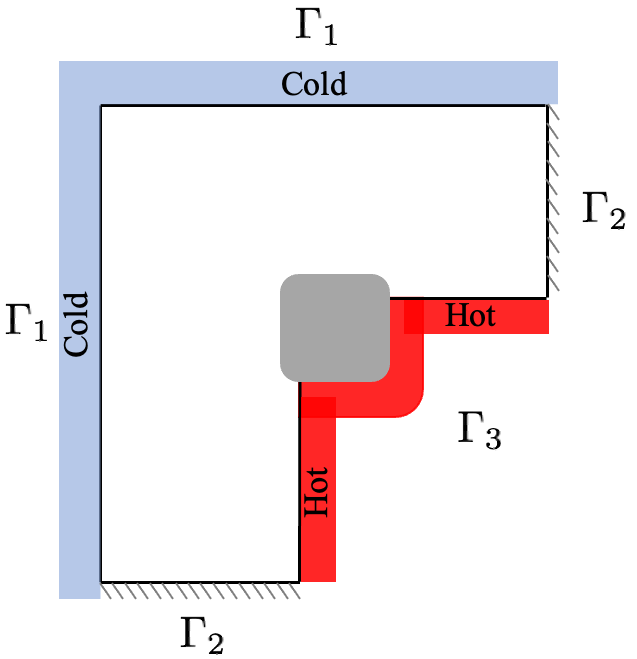
\includegraphics[width=0.45\textwidth]{Figures/Thermal_BC_IB2.png}\hspace{0.1 in}
    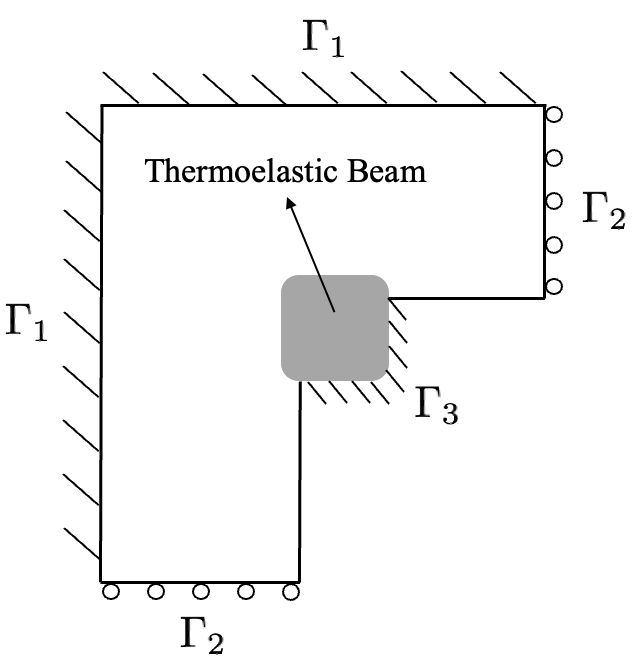
\includegraphics[width=0.45\textwidth]{Figures/Mechanical_BC_IB2.png}\\
    Thermal Scenario \hspace{1.2 in} Mechanical Scenario\\
\end{center}
\end{frame}
%================================================================================
%================================================================================
\begin{frame}{Results: Comparison}
\begin{figure}
        \centering
        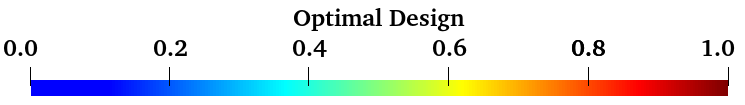
\includegraphics[width=0.35\linewidth]{Figures/design_contour_2.png}
    \end{figure}
    \vspace{-0.1in}\\
    \begin{figure}
        \centering
        \footnotesize
        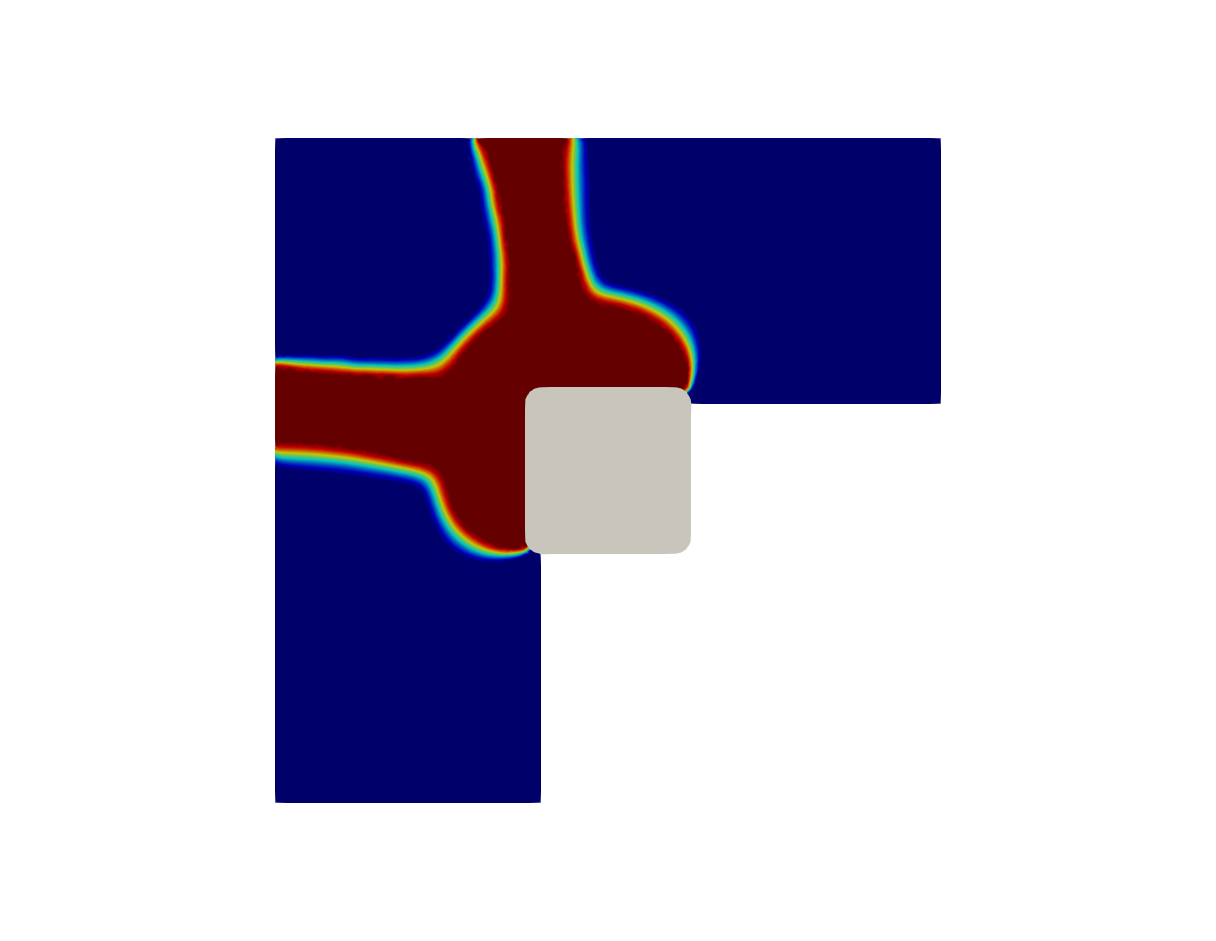
\includegraphics[trim={3.6in 1.8in 3.5in 2.5in},clip,width=0.25\linewidth]{Figures/LU1.png}\hspace{0.1in}~
        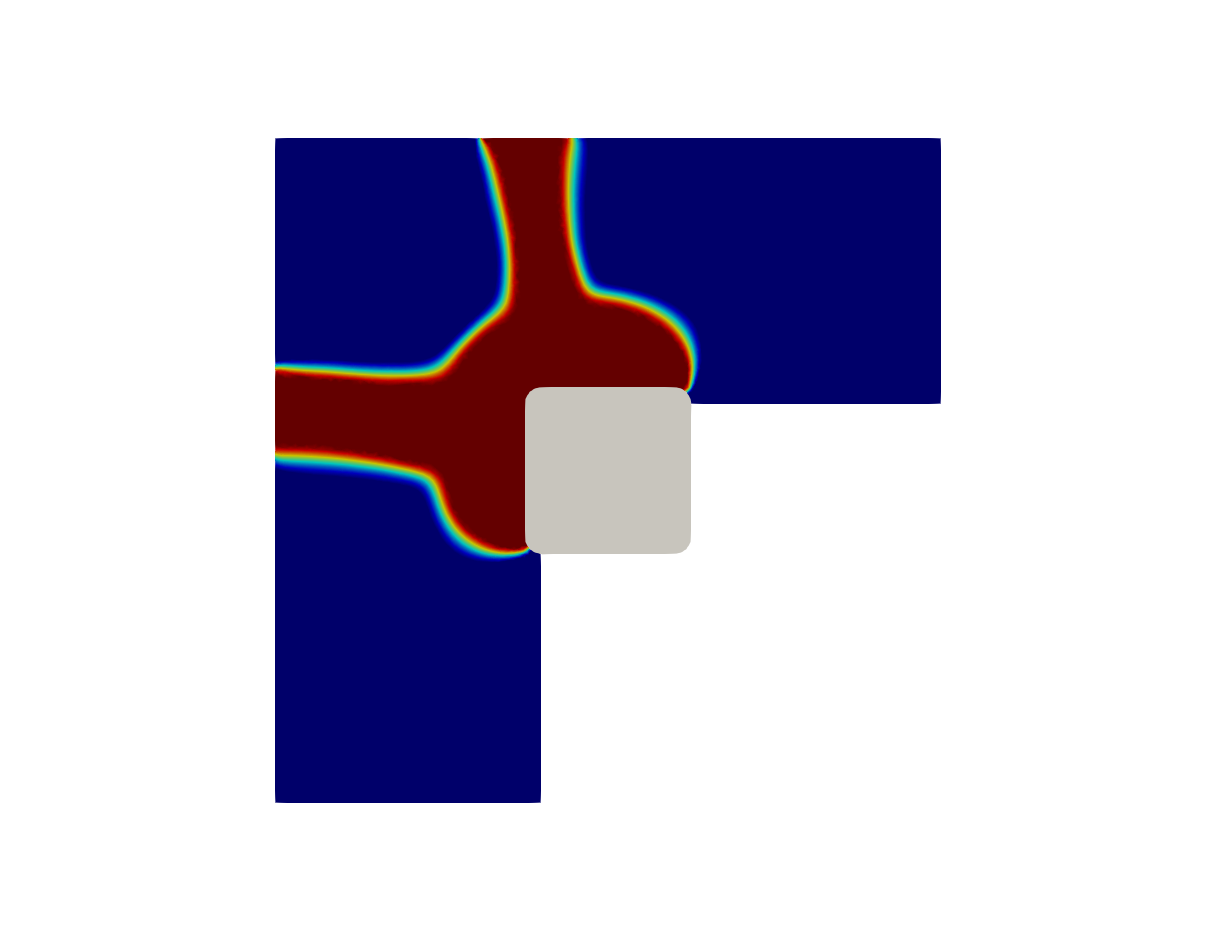
\includegraphics[trim={3.6in 1.8in 3.5in 2.5in},clip,width=0.25\linewidth]{Figures/LU2.png}\hspace{0.1in}~
        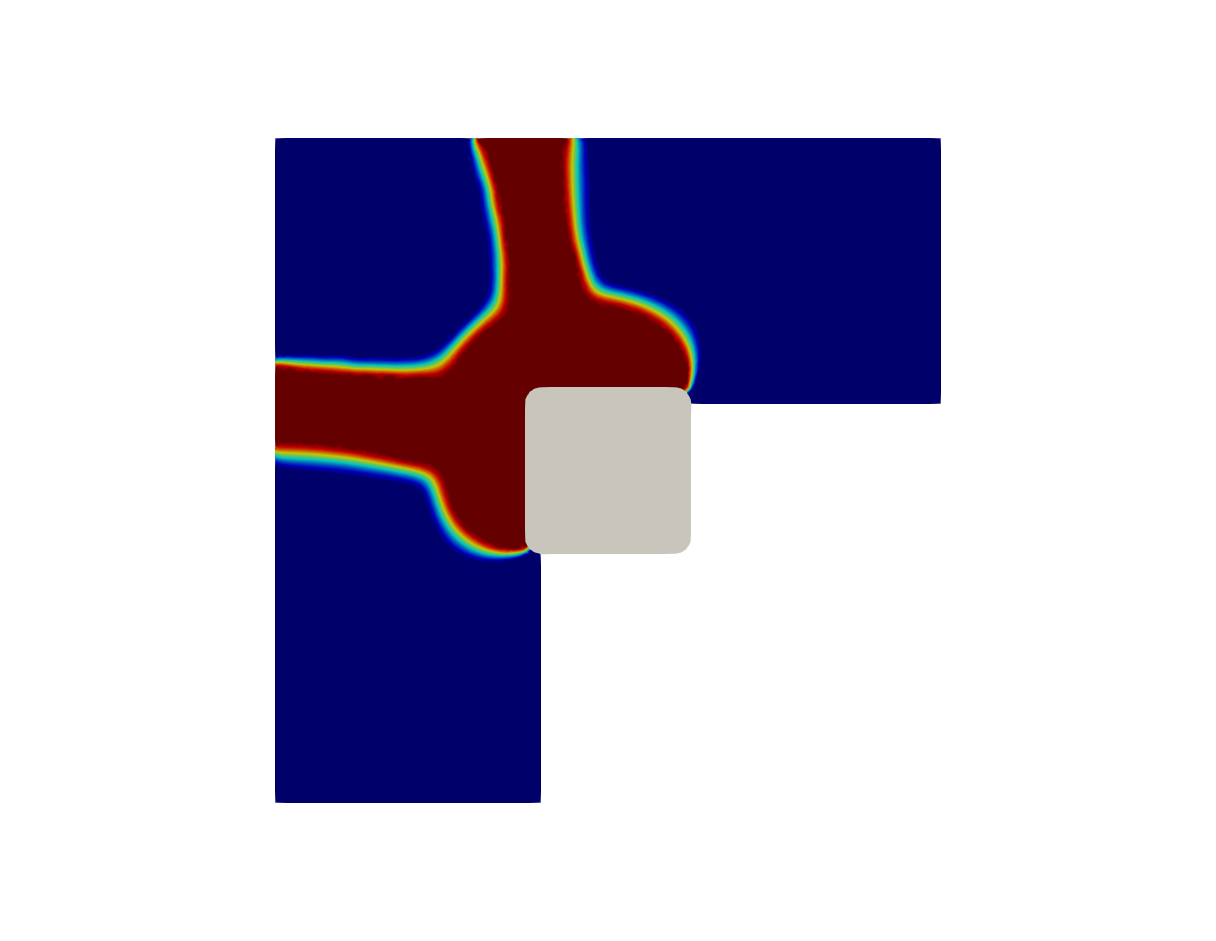
\includegraphics[trim={3.6in 1.8in 3.5in 2.5in},clip,width=0.25\linewidth]{Figures/LU3.png}\\
        \footnotesize{Monte Carlo \hspace{0.6 in} { Control Variate} \hspace{0.6 in} Quadratic } \vspace{0.1 in}\\
        \fbox{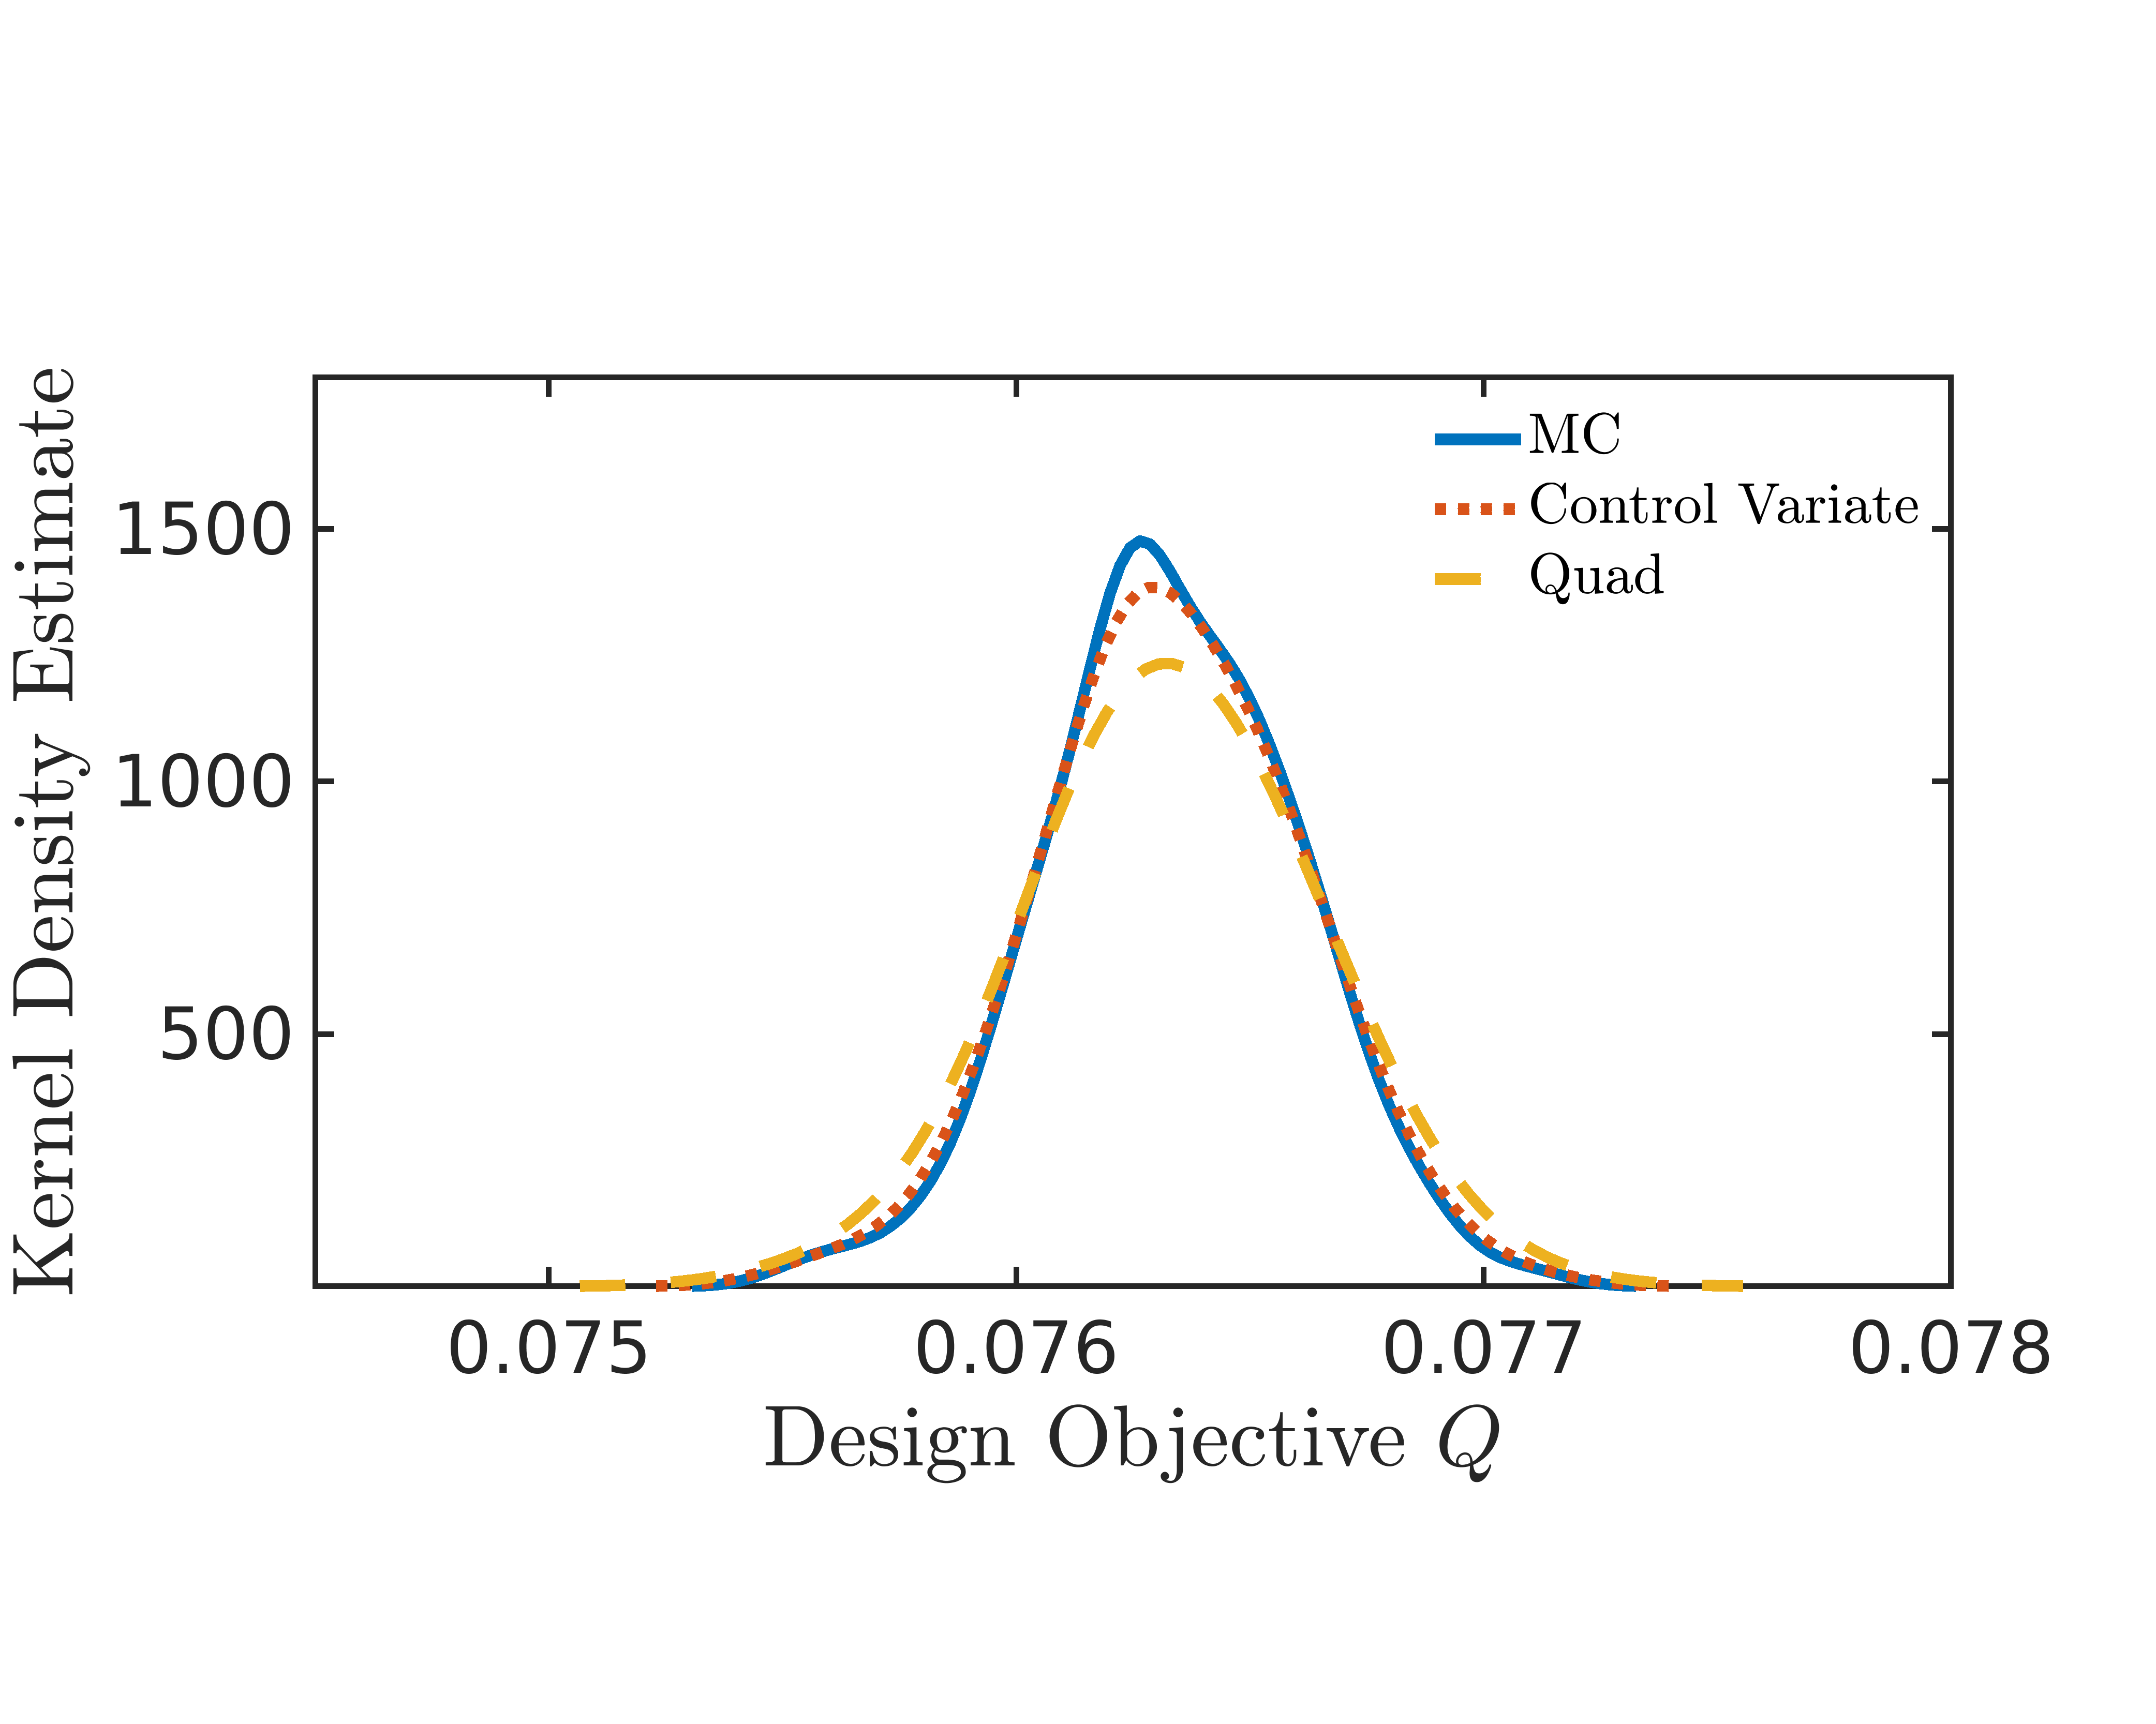
\includegraphics[trim={0in 1in 0in 1.5in},clip,width=0.4\linewidth]{Figures/L1_4.png}}
        \label{fig:enter-label}
    \end{figure}
    \centering
    $L_c = 0.25, \: \red{\sigma= 0.25},\: \alpha_c = 0.1, \:T_{cr} = 22.5 \:\text{MPa},\: \beta_{V} = 1$
\end{frame}
%===============================================================
%===============================================================
\begin{frame}{Results: Comparison}
\begin{figure}
        \centering
        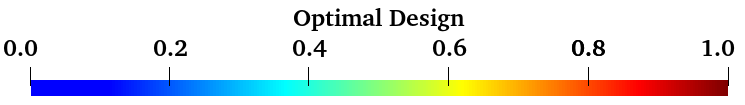
\includegraphics[width=0.35\linewidth]{Figures/design_contour_2.png}
    \end{figure}
    \vspace{-0.1in}\\
    \begin{figure}
        \centering
        \footnotesize
        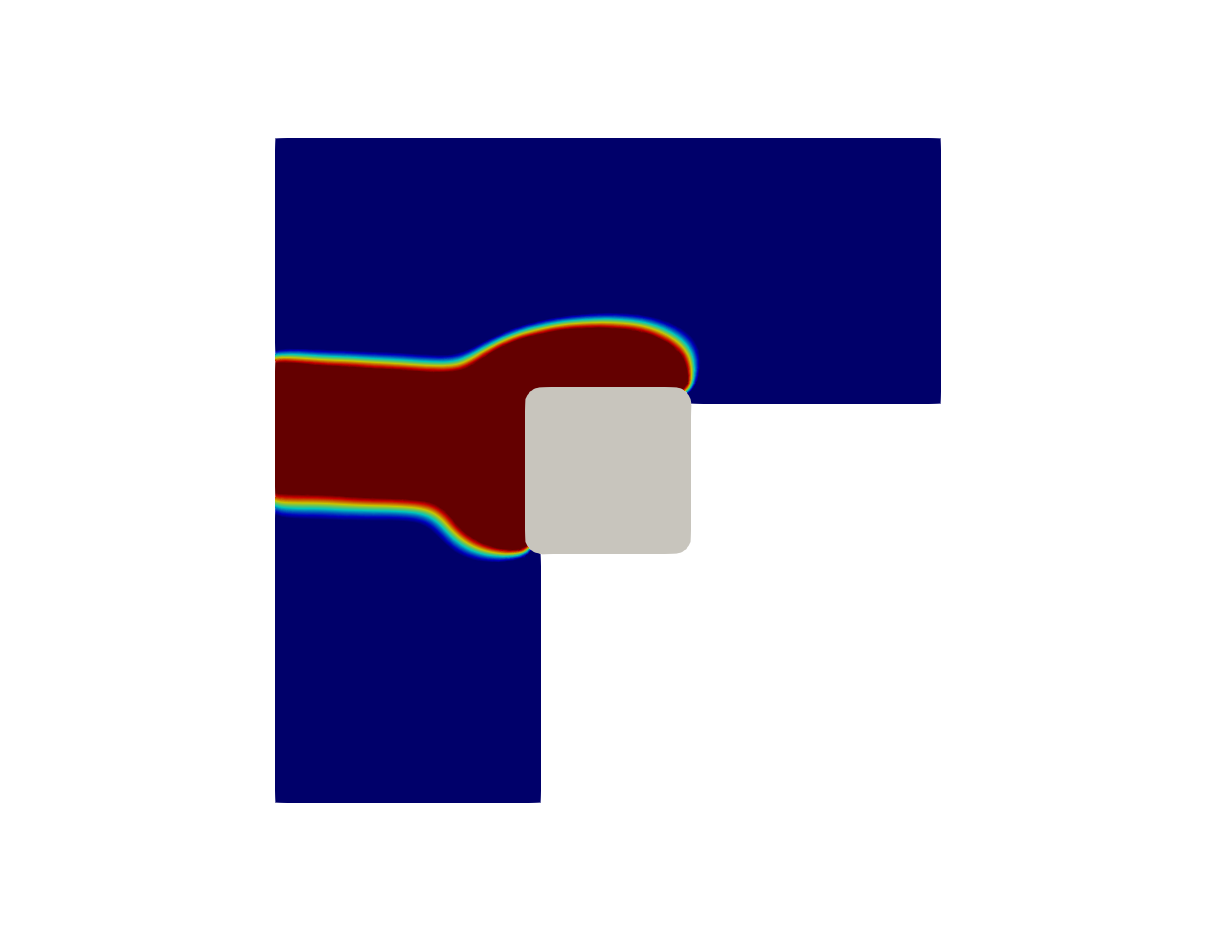
\includegraphics[trim={3.6in 1.8in 3.5in 2.5in},clip,width=0.25\linewidth]{Figures/HU1.png}\hspace{0.1in}~
        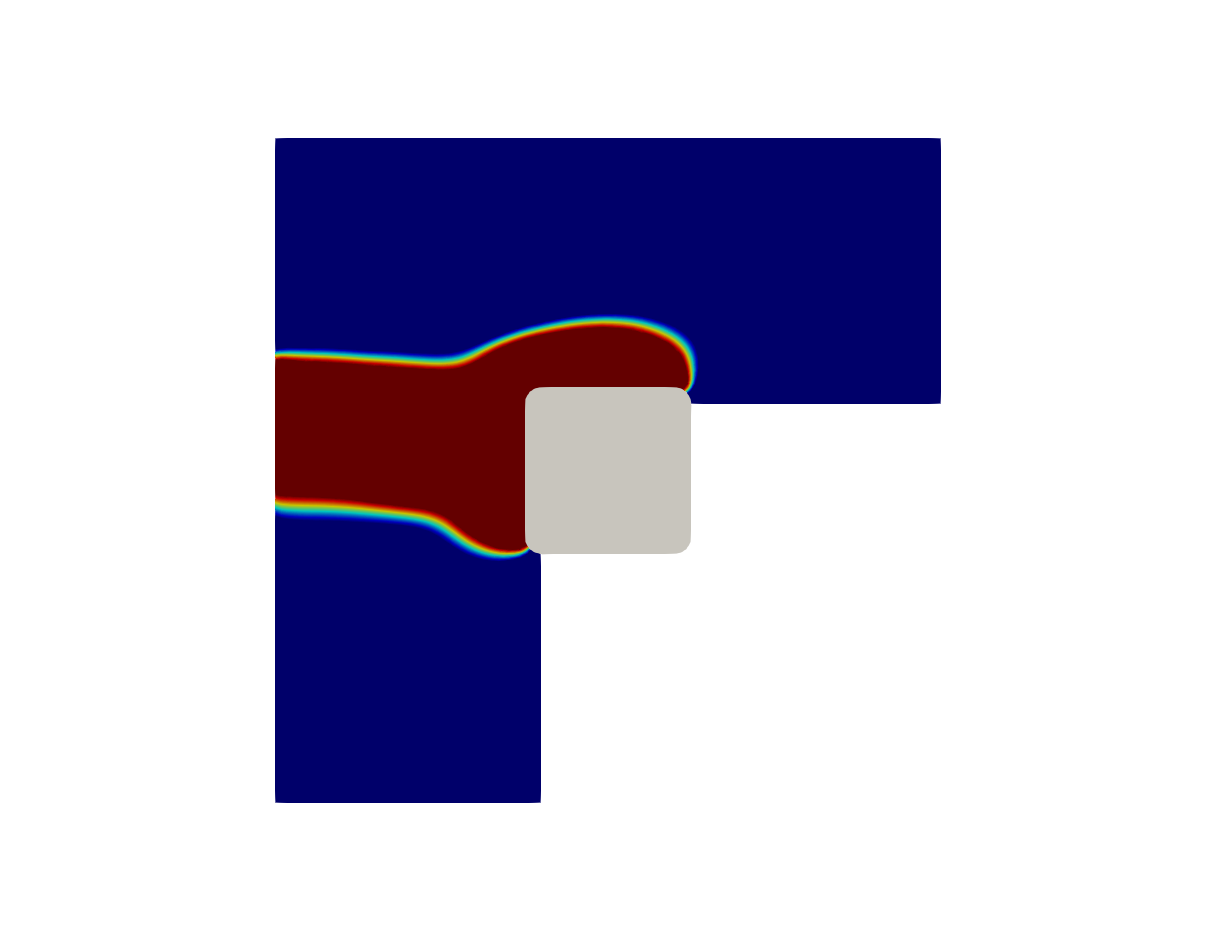
\includegraphics[trim={3.6in 1.8in 3.5in 2.5in},clip,width=0.25\linewidth]{Figures/HU2.png}\hspace{0.1in}~
        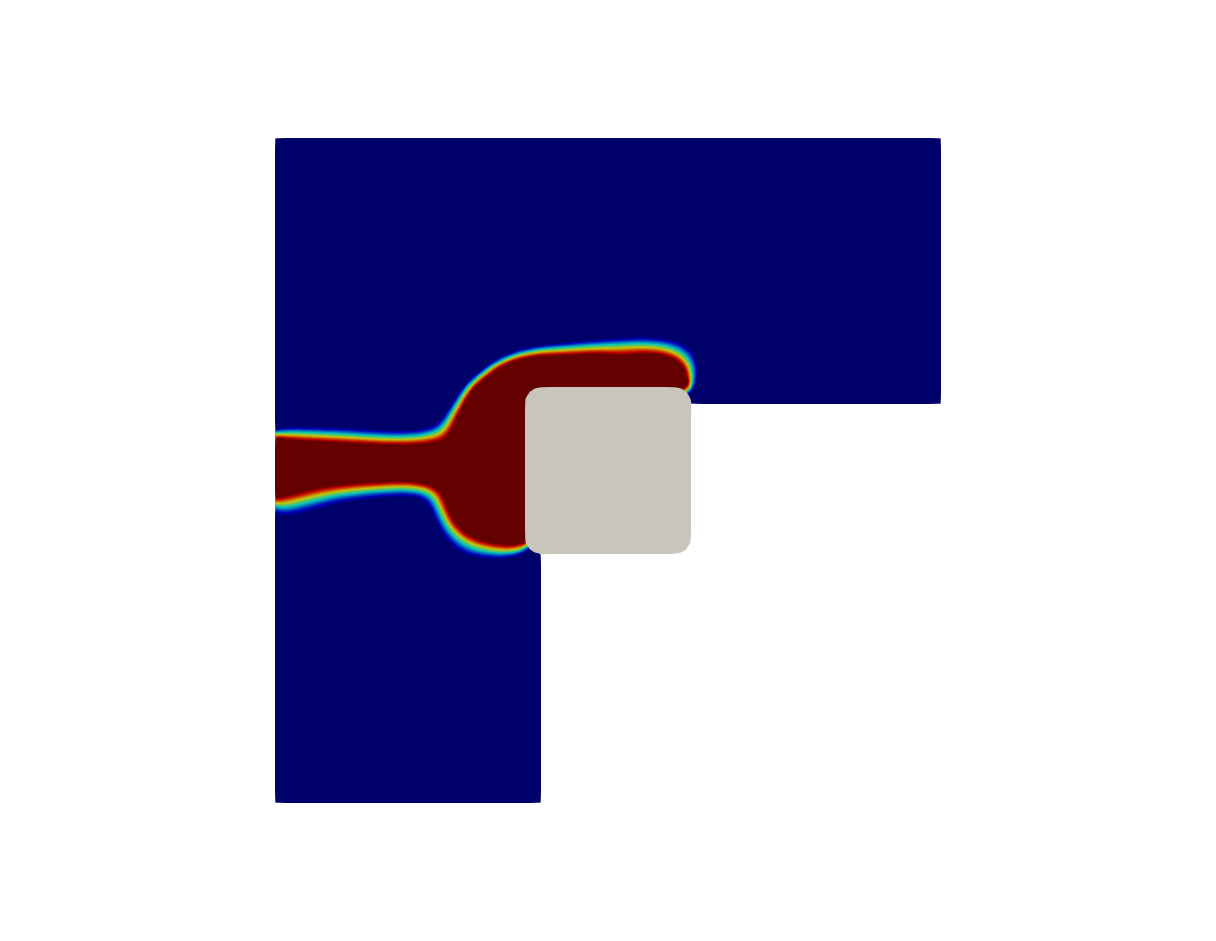
\includegraphics[trim={3.6in 1.8in 3.5in 2.5in},clip,width=0.25\linewidth]{Figures/HU3.png}\\
        \footnotesize{Monte Carlo \hspace{0.6 in} { Control Variate} \hspace{0.6 in} Quadratic } \vspace{0.1 in}\\
        \fbox{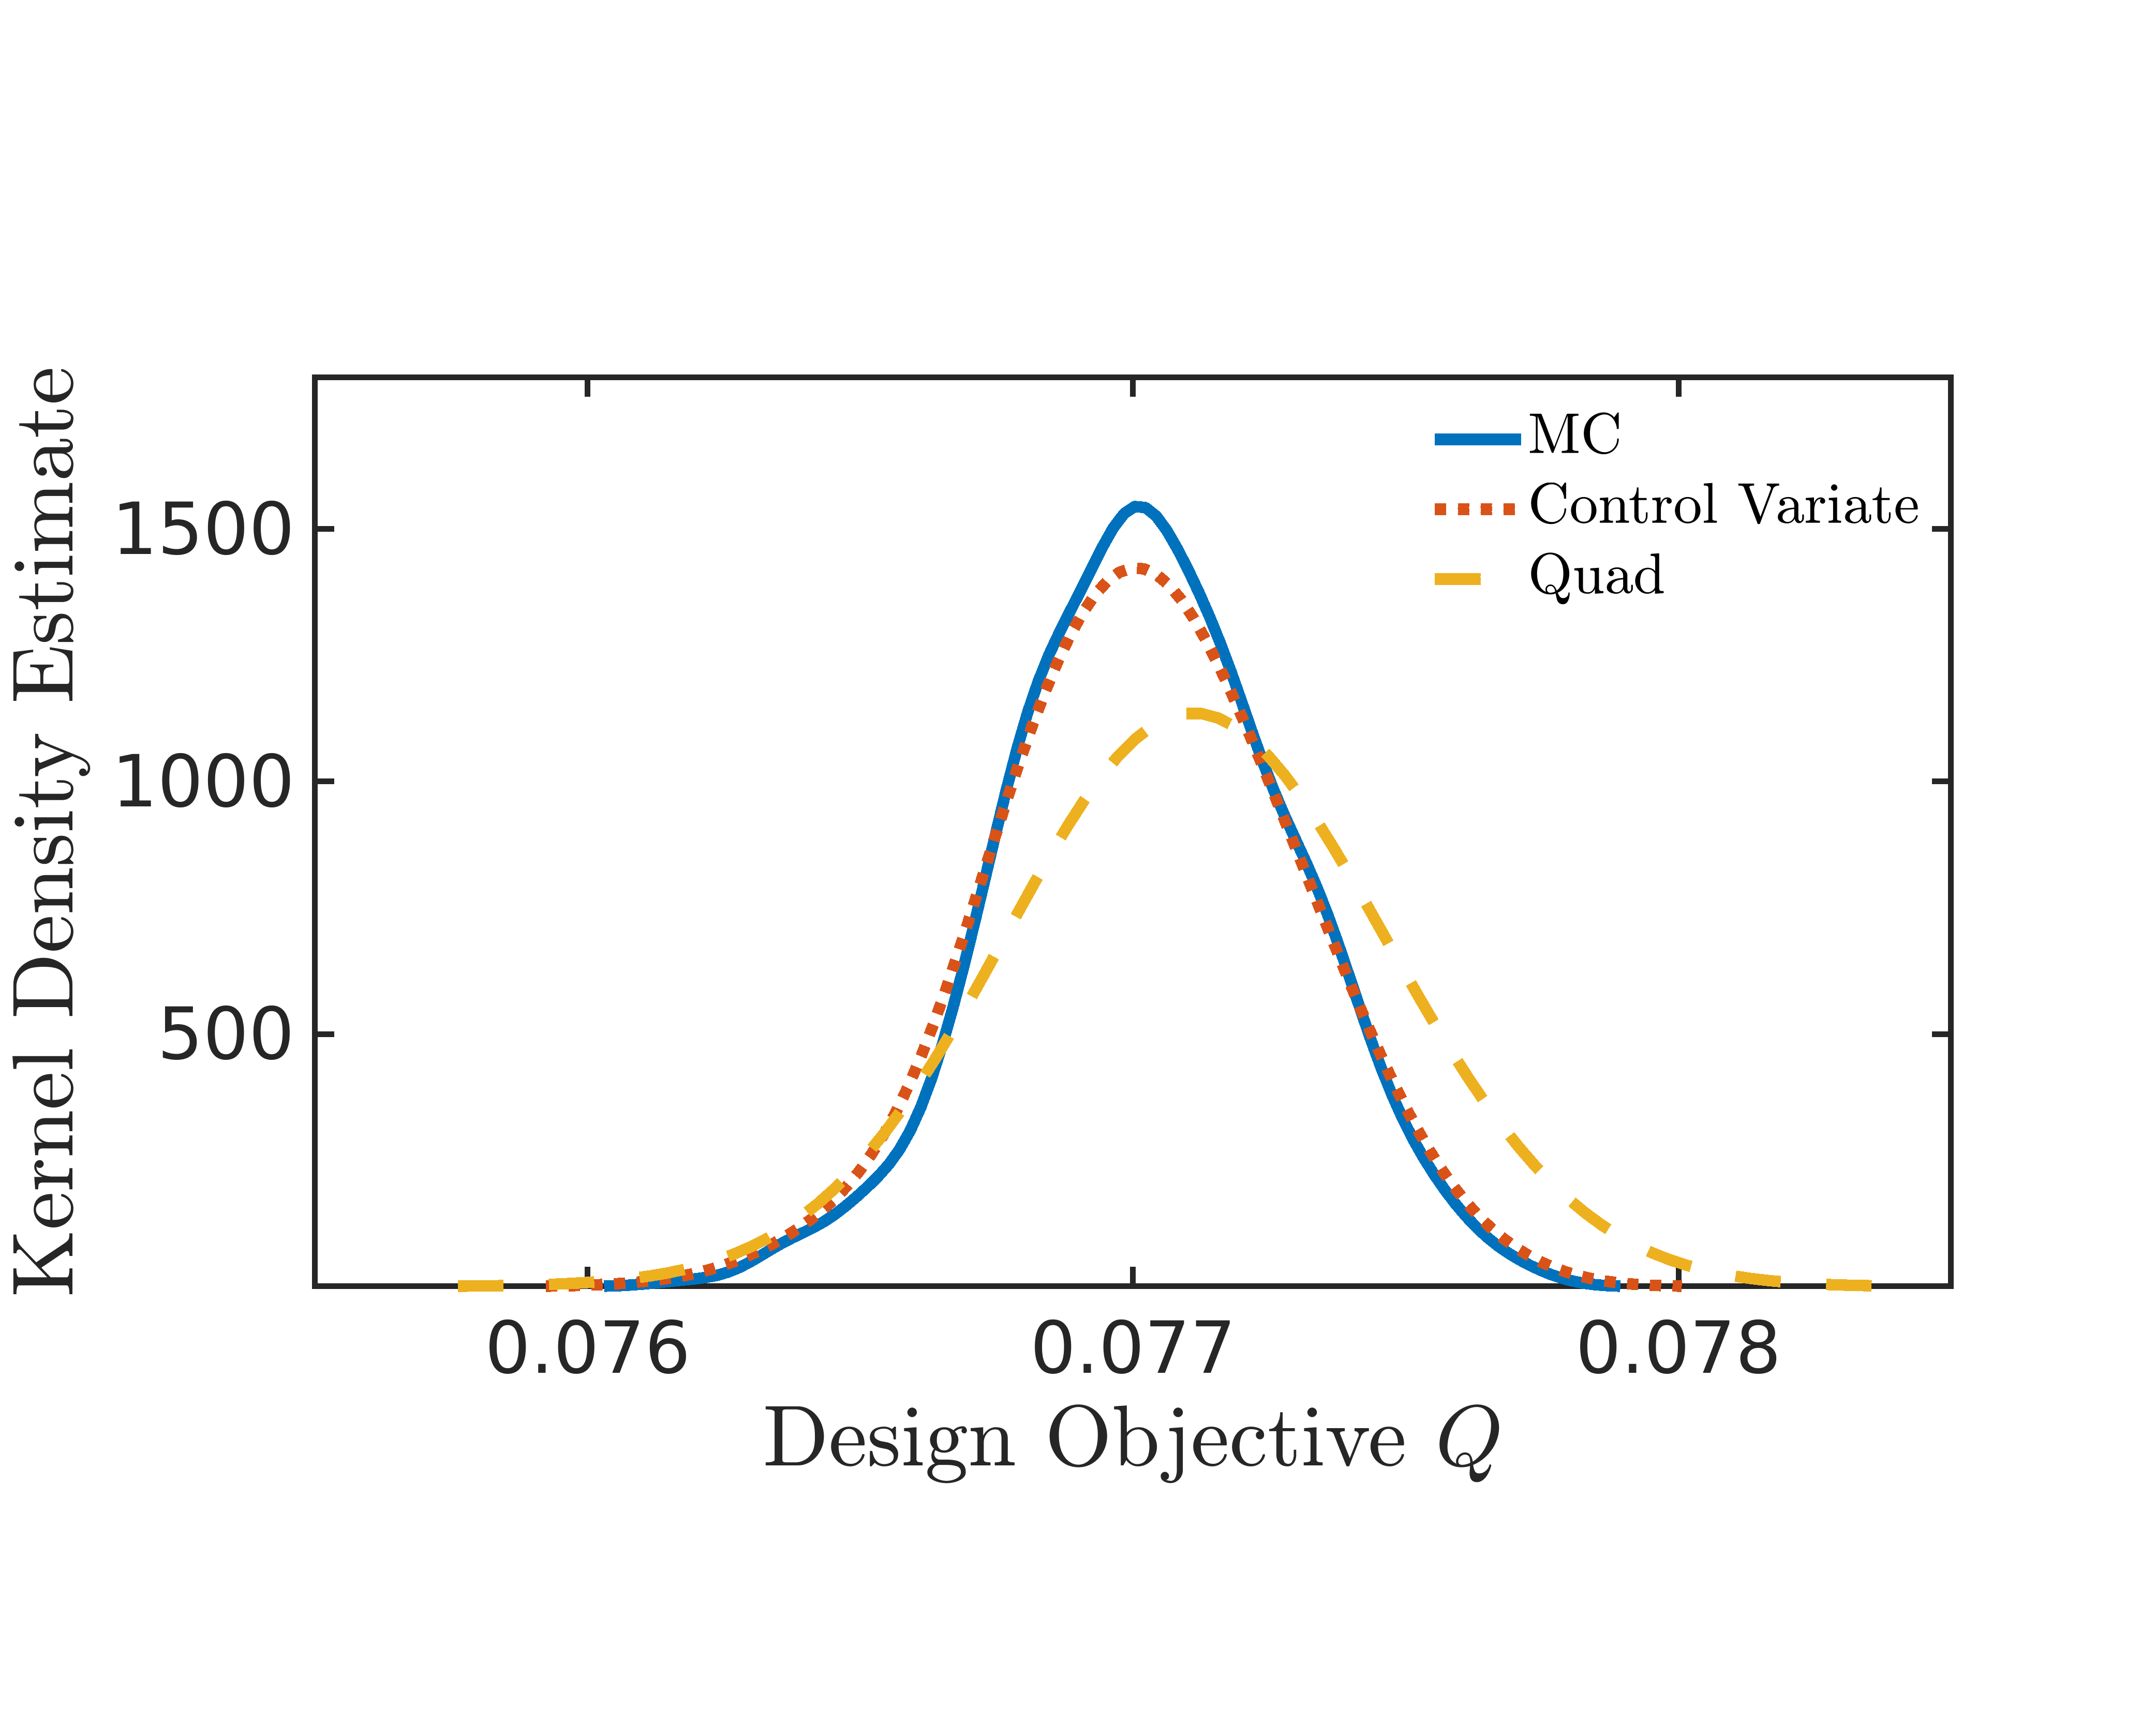
\includegraphics[trim={0in 1in 0in 1.5in},clip,width=0.4\linewidth]{Figures/H1_4.png}}
        \label{fig:enter-label}
    \end{figure}
    \centering
    $L_c = 0.25, \: \red{\sigma= 0.5},\: \alpha_c = 0.1, \:T_{cr} = 22.5 \:\text{MPa},\: \beta_{V} = 1$
\end{frame}
%==============================================================
%================================================================================

\begin{frame}{Results: Effect of critical stress}
\centering
    \begin{figure}
        \centering
        \footnotesize
        \begin{tabular}{c c c c}
        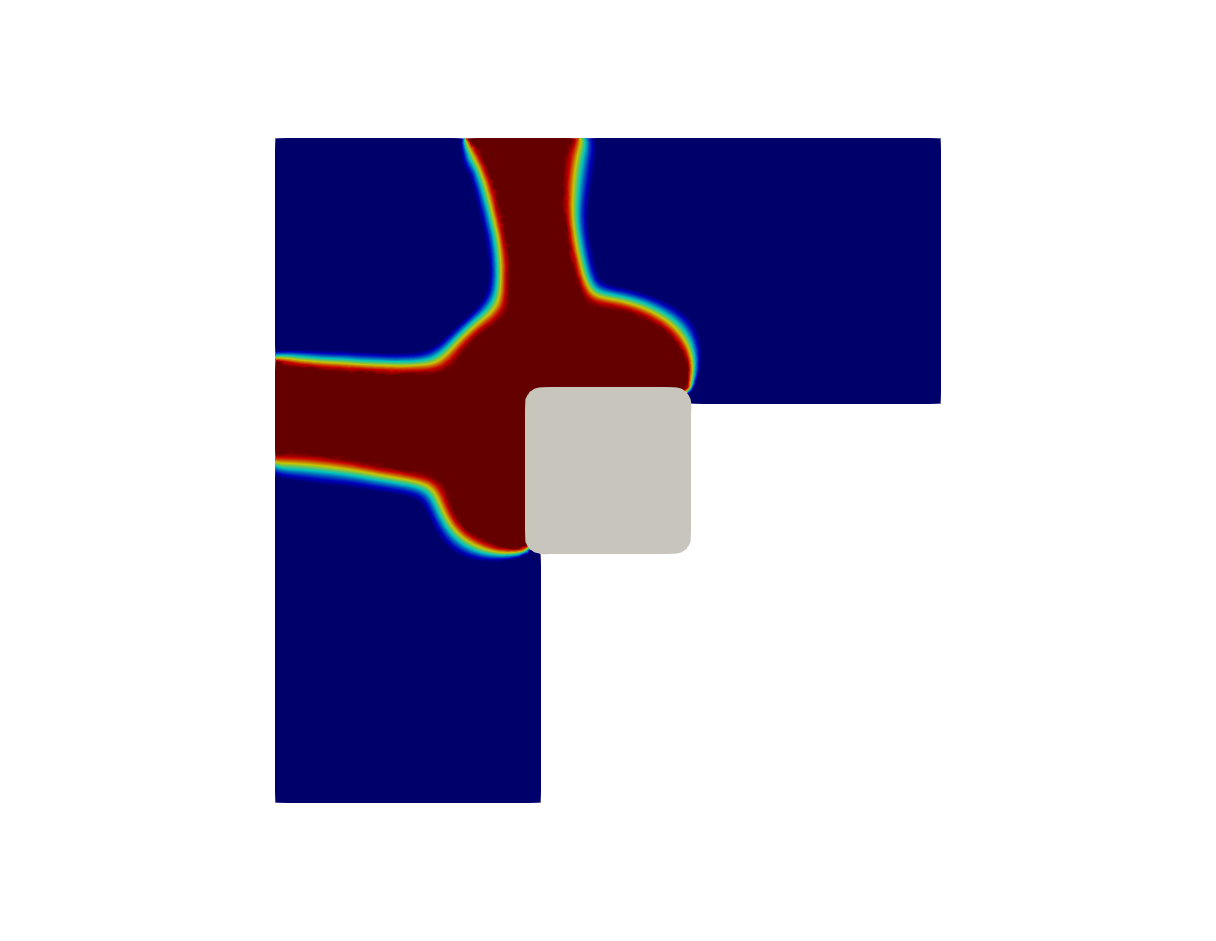
\includegraphics[trim={3.6in 1.8in 3.5in 2.5in},clip,width=0.2\textwidth]{Figures/CS1.png}&
        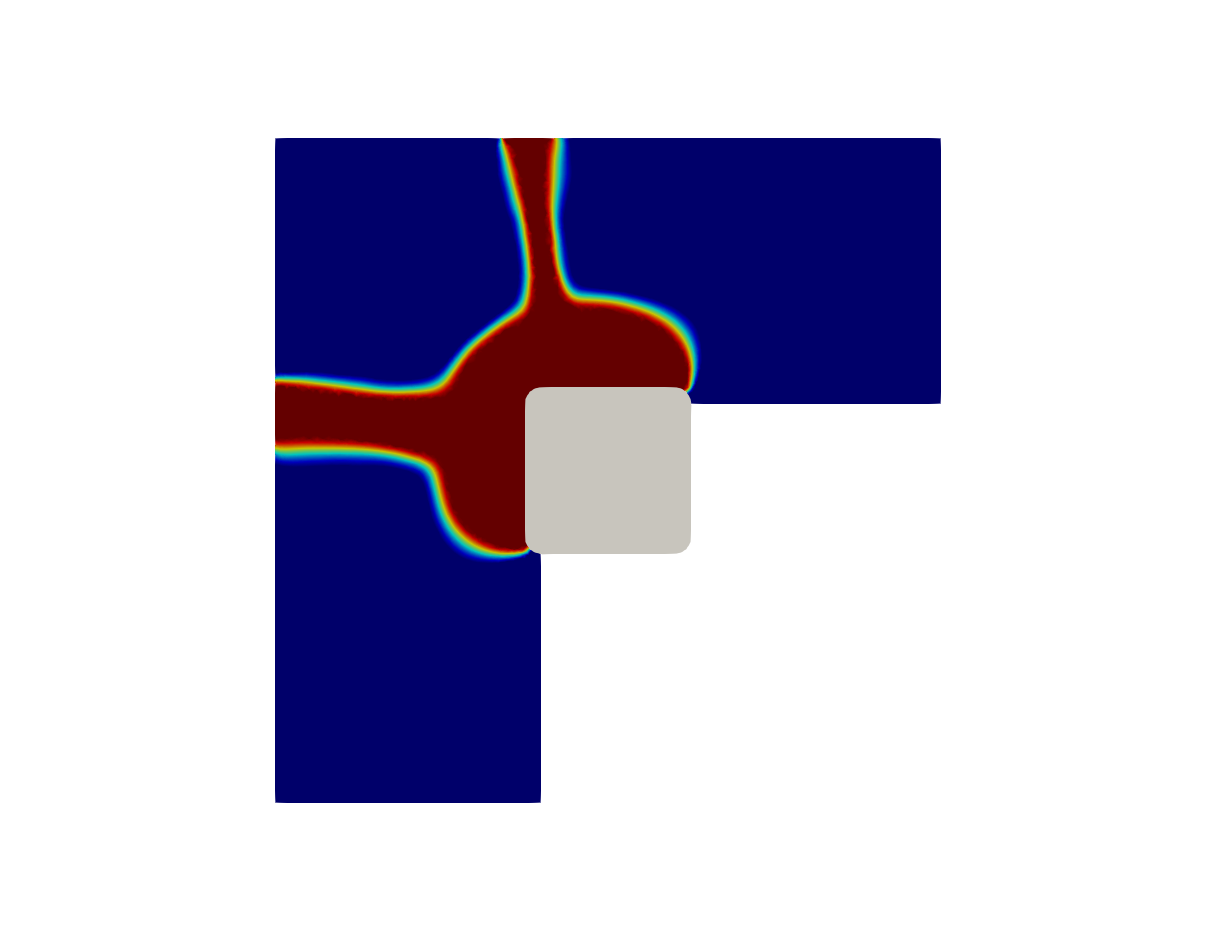
\includegraphics[trim={3.6in 1.8in 3.5in 2.5in},clip,width=0.2\textwidth]{Figures/CS2.png}&
        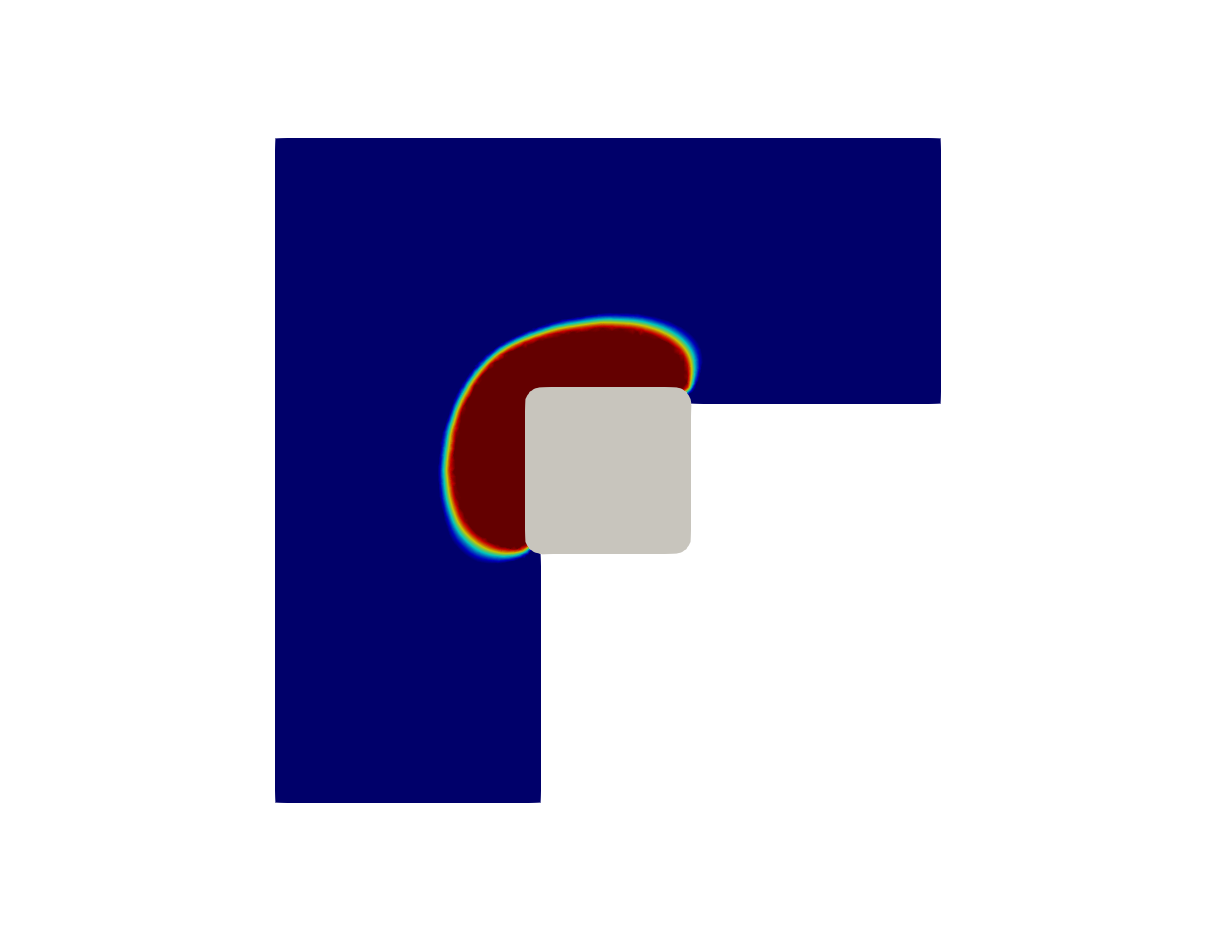
\includegraphics[trim={3.6in 1.8in 3.5in 2.5in},clip,width=0.2\textwidth]{Figures/CS3.png}&
        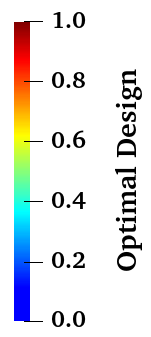
\includegraphics[width=0.06\textwidth]{Figures/design_contour.png}
        \\
        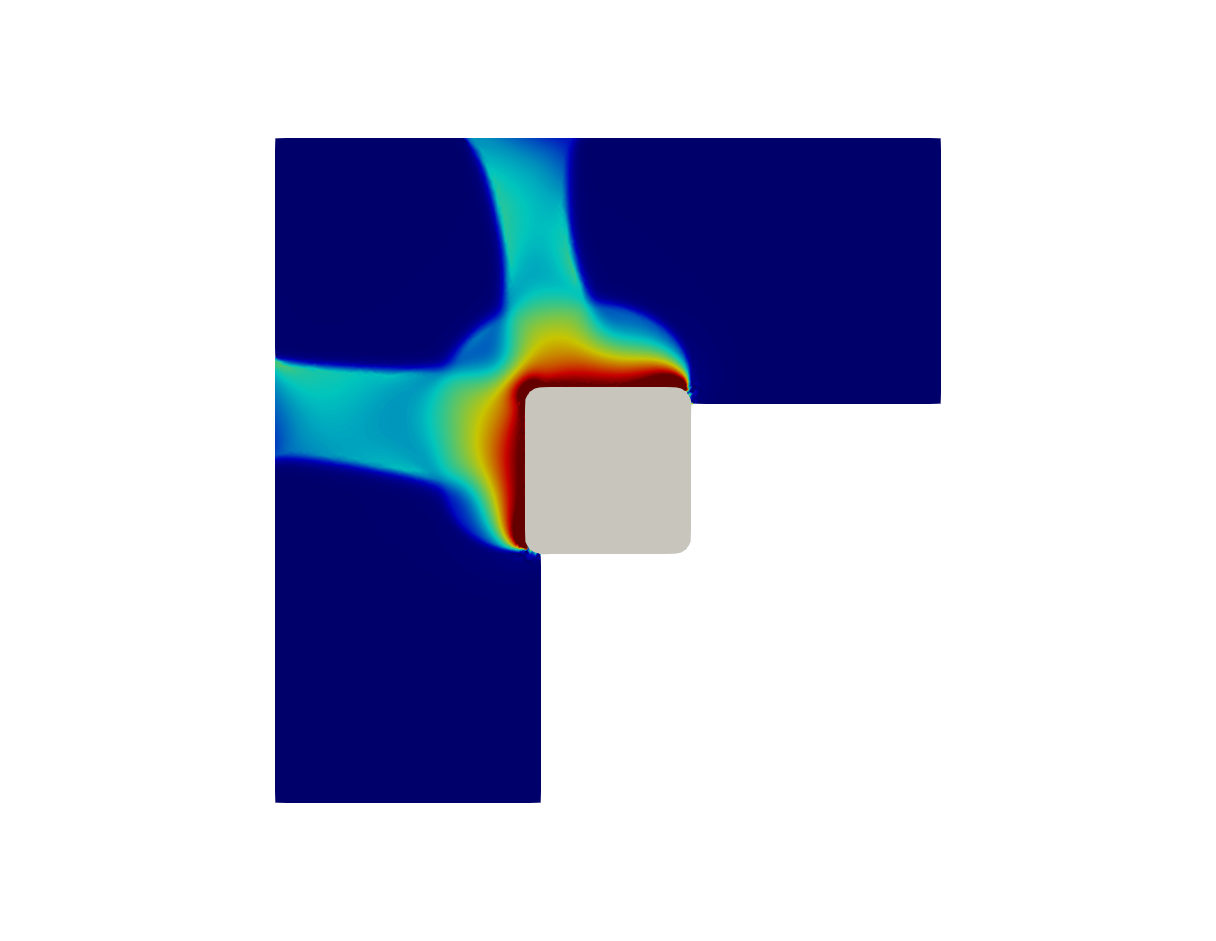
\includegraphics[trim={3.6in 1.8in 3.5in 2.5in},clip,width=0.2\textwidth]{Figures/Stress_CS1.png}&
        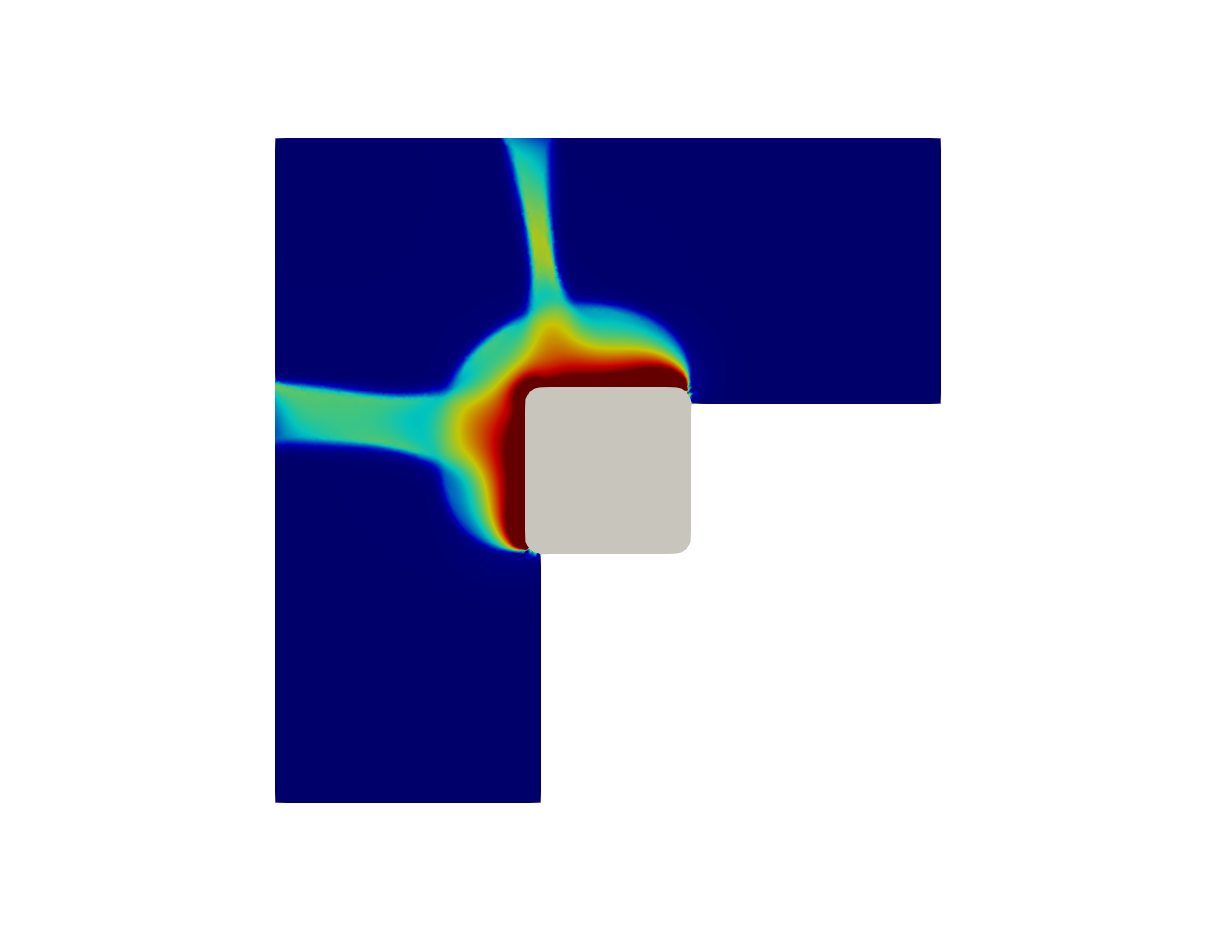
\includegraphics[trim={3.6in 1.8in 3.5in 2.5in},clip,width=0.2\textwidth]{Figures/Stress_CS2.png}&
        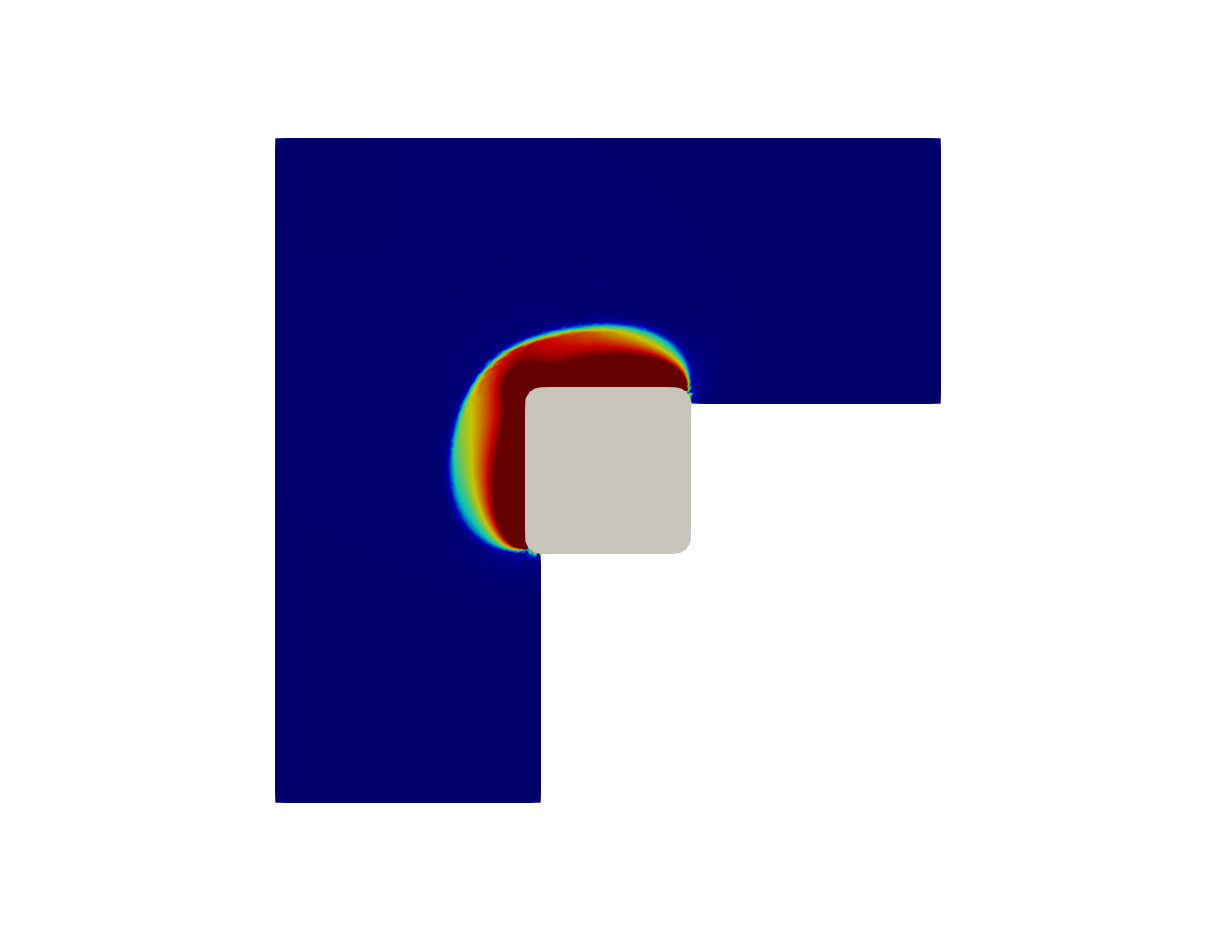
\includegraphics[trim={3.6in 1.8in 3.5in 2.5in},clip,width=0.2\textwidth]{Figures/Stress_CS3.png}&
        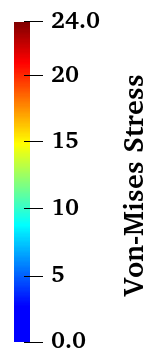
\includegraphics[width=0.06\textwidth]{Figures/CS_contour.png}
        \\
        $T_{cr} = 20 \: \text{MPa}$ &  $T_{cr} = 22.5 \: \text{MPa}$ & $T_{cr} = 25 \: \text{MPa}$ &\\
       \end{tabular}
        \label{fig:1}
    \end{figure}
    \fbox{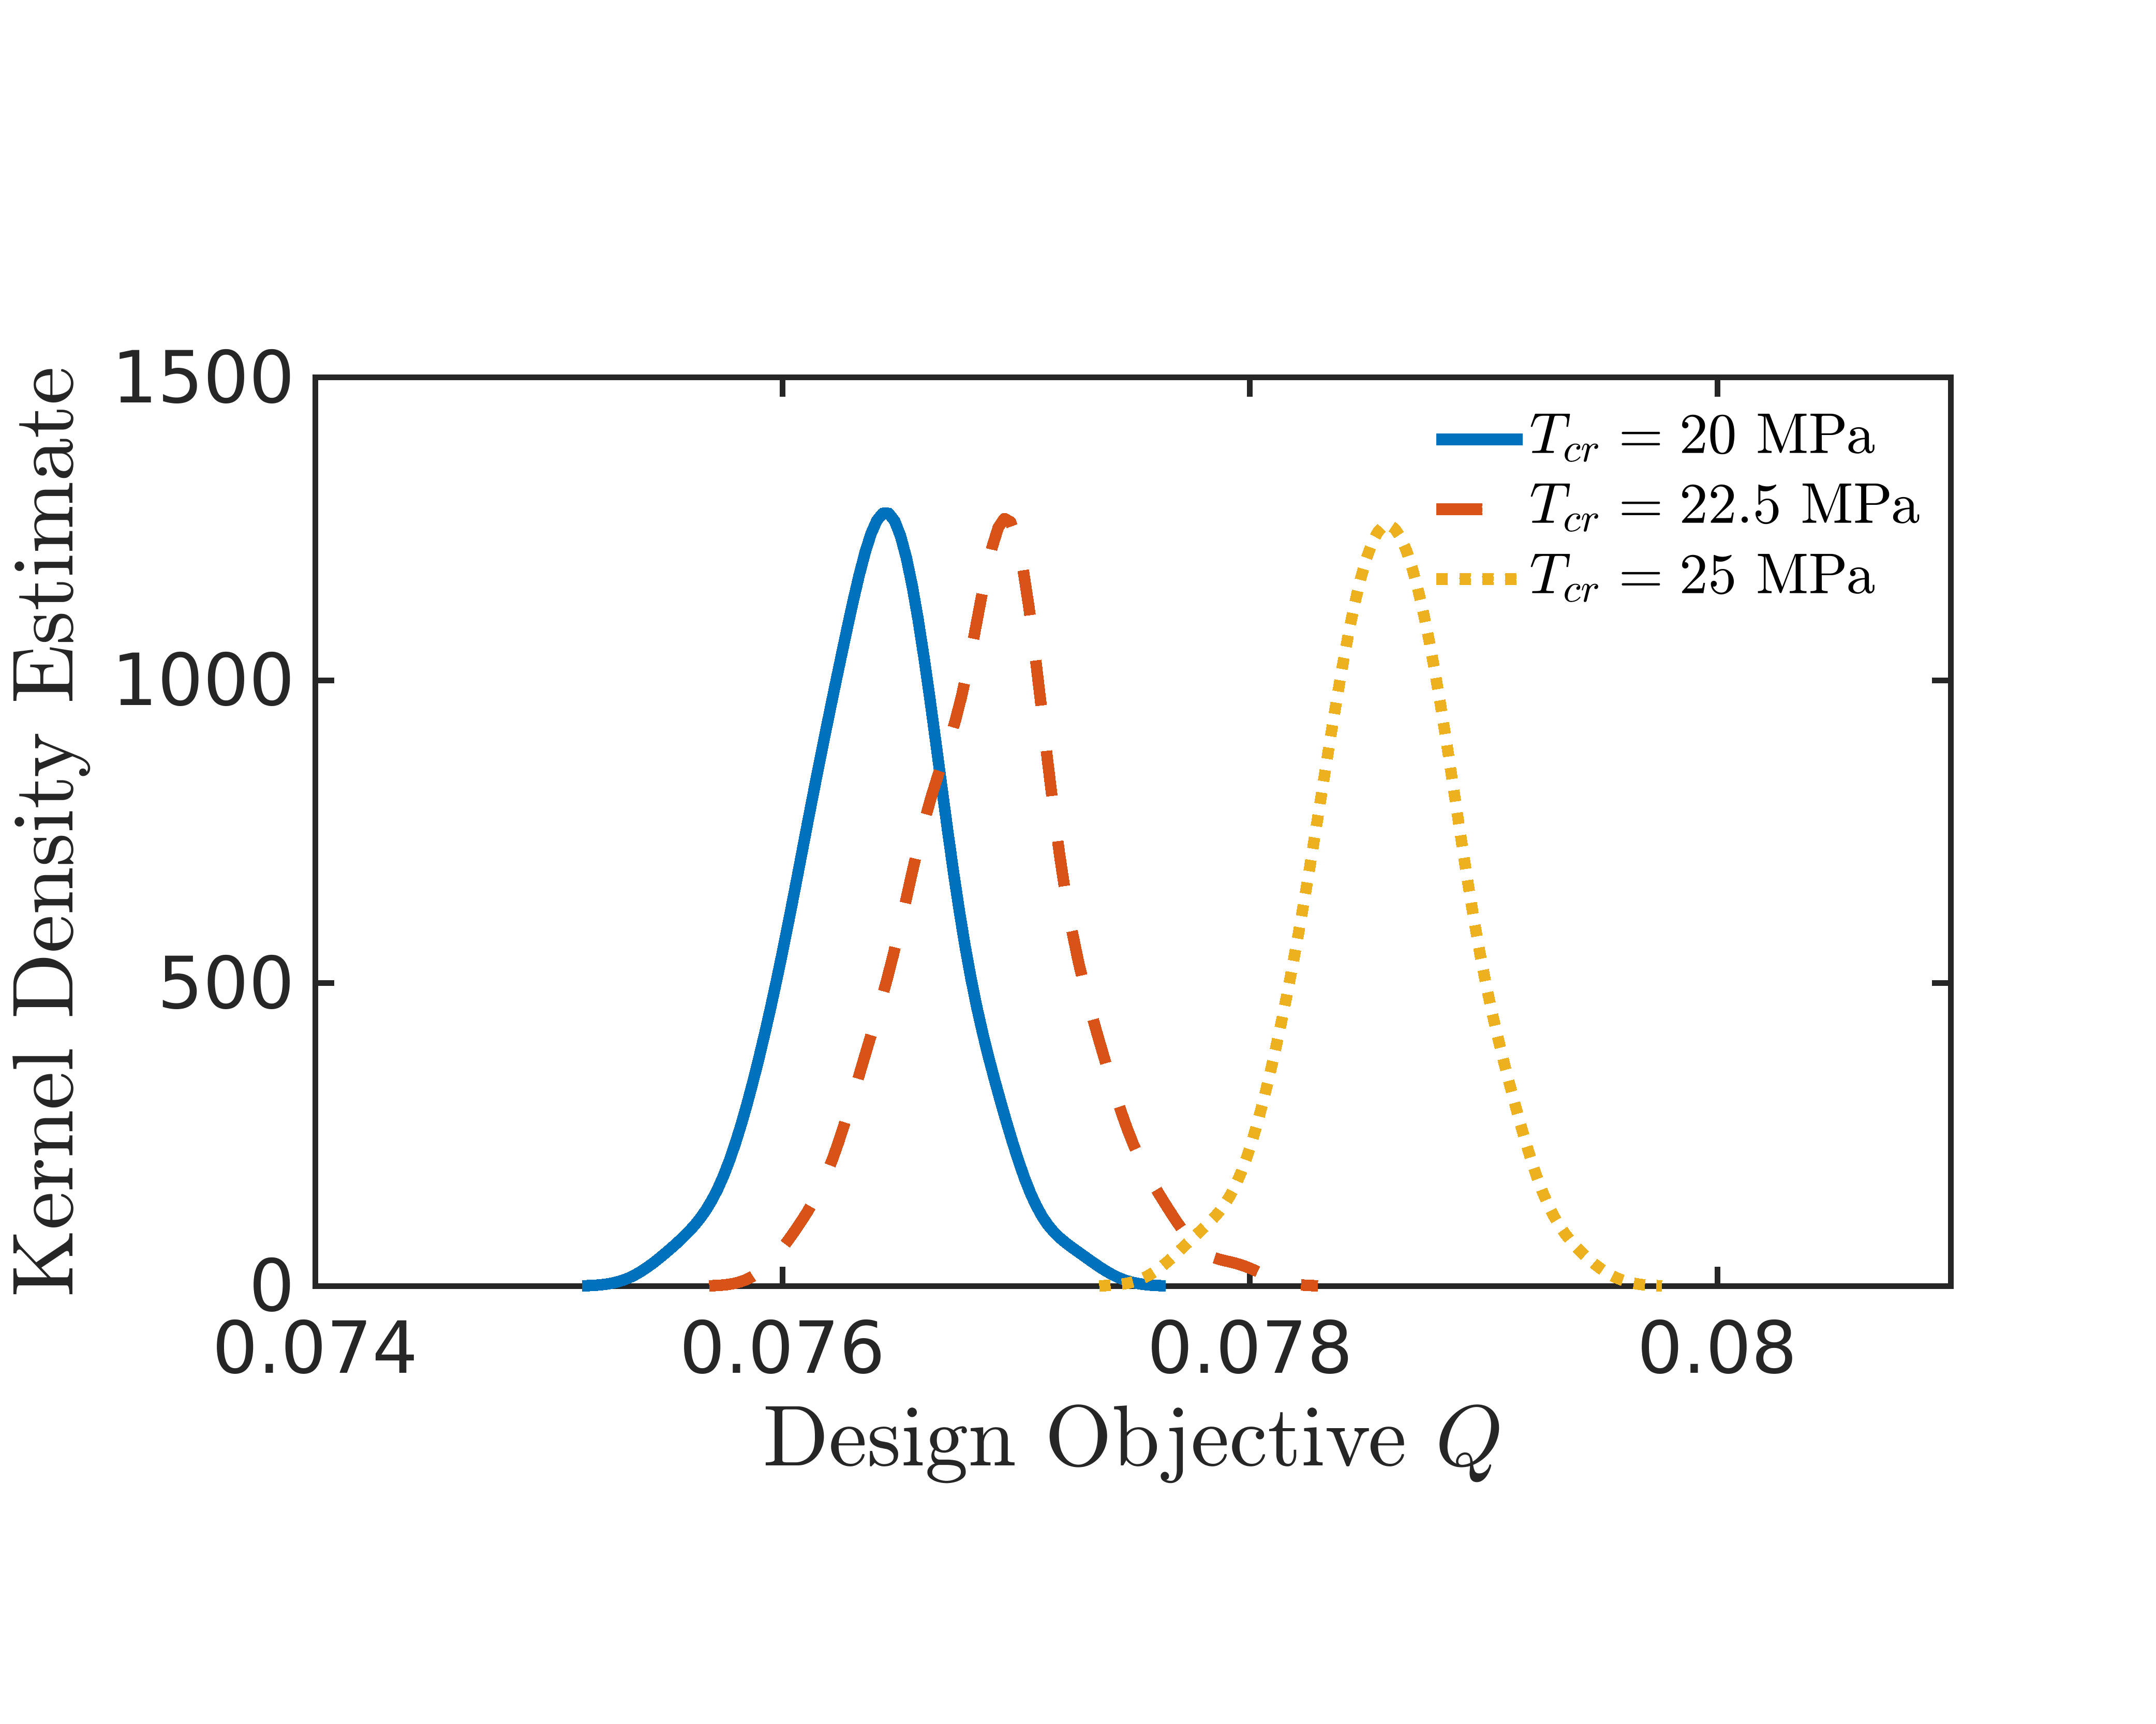
\includegraphics[trim={0in 1in 0in 1.5in},clip,width=0.4\linewidth]{Figures/critical_stress.png}}
    %$\alpha_c = 0.1, \beta_{tik}= 1e-4, \sigma_{\gamma}= 10, \sigma_{\beta}=4, L_c = 0.05, \sigma=0.1, \beta_V =0.1$
\end{frame}


\begin{frame}{Results: Effect of critical chance}
\centering
    \begin{figure}
        \centering
        \footnotesize
        \begin{tabular}{c c c c}
        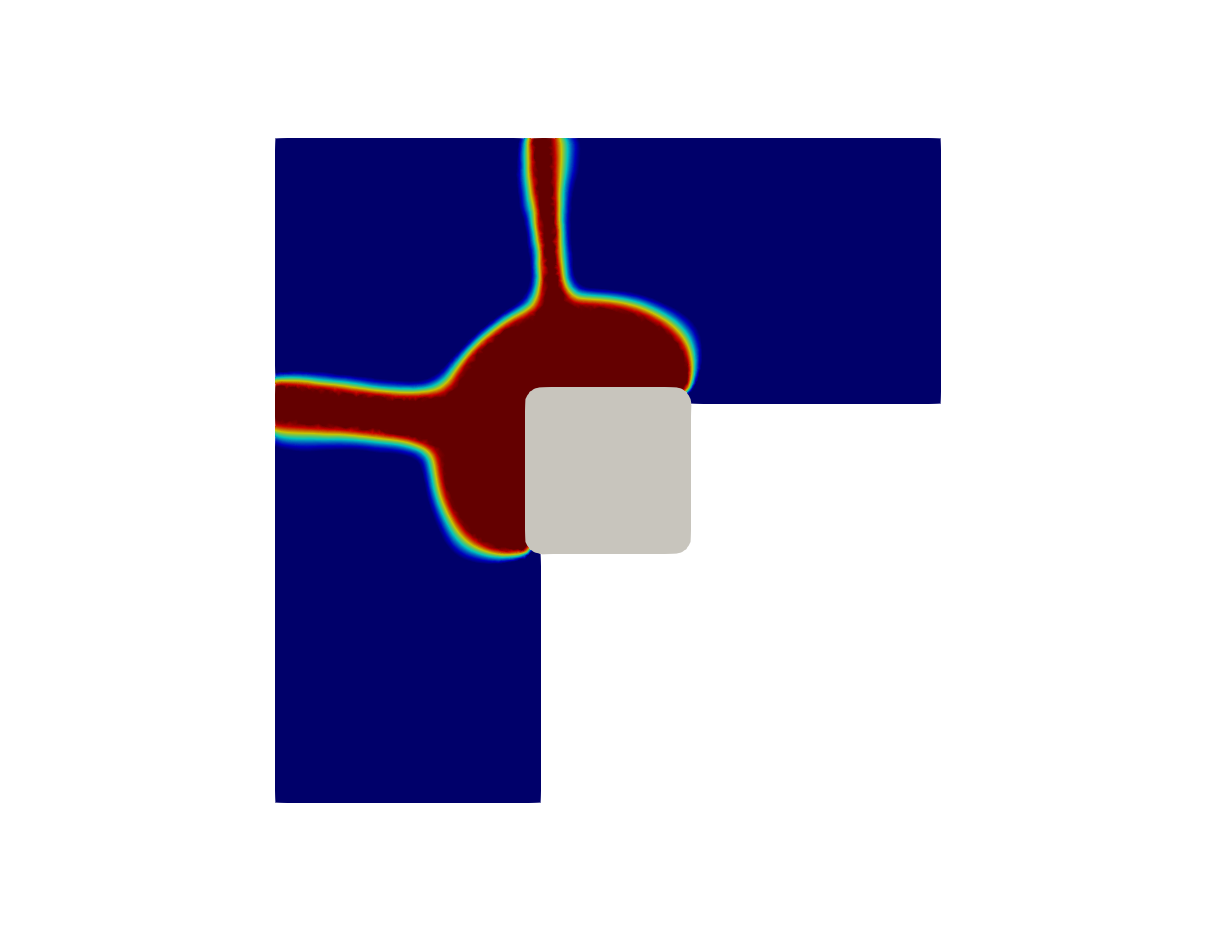
\includegraphics[trim={3.6in 1.8in 3.5in 2.5in},clip,width=0.2\textwidth]{Figures/CC1.png}&
        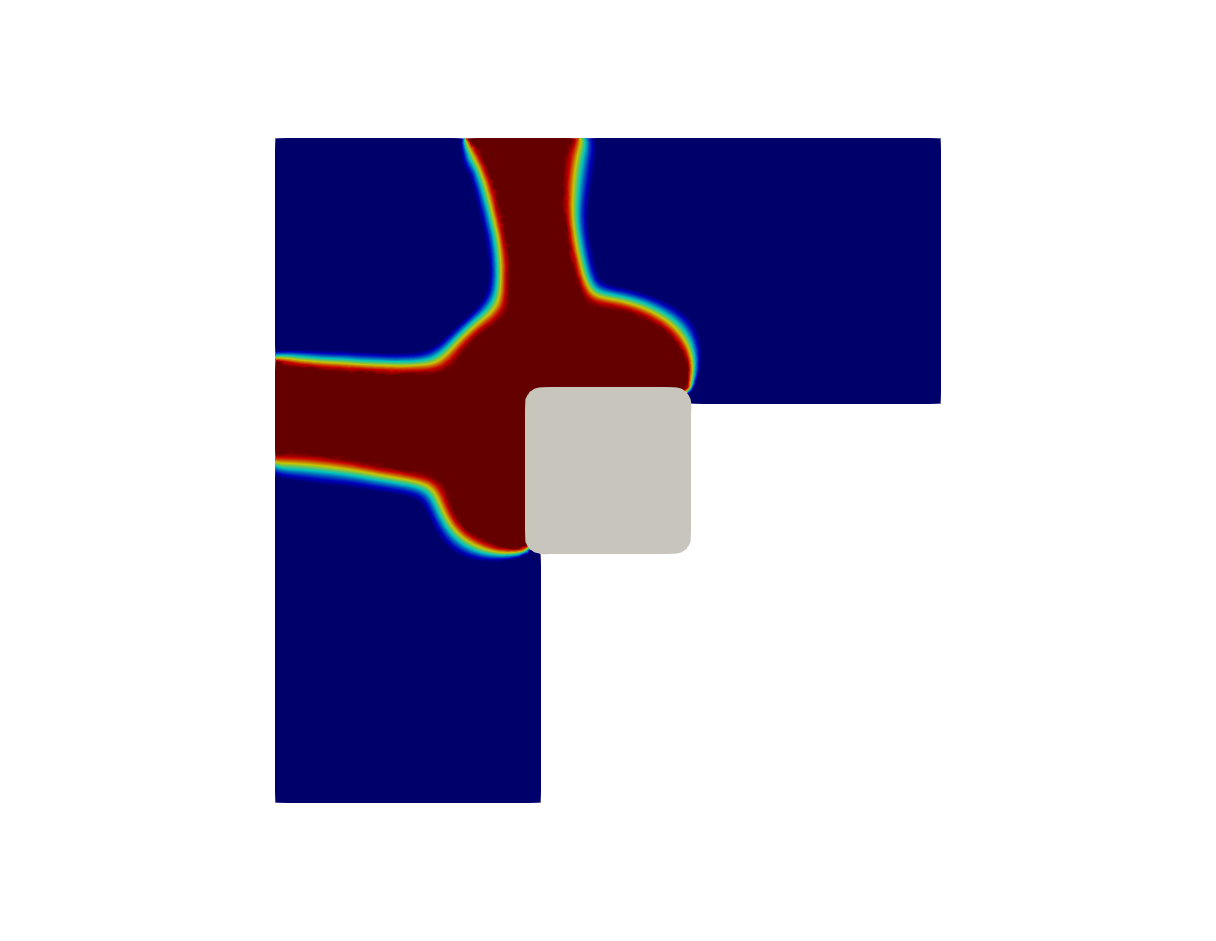
\includegraphics[trim={3.6in 1.8in 3.5in 2.5in},clip,width=0.2\textwidth]{Figures/CC2.png}&
        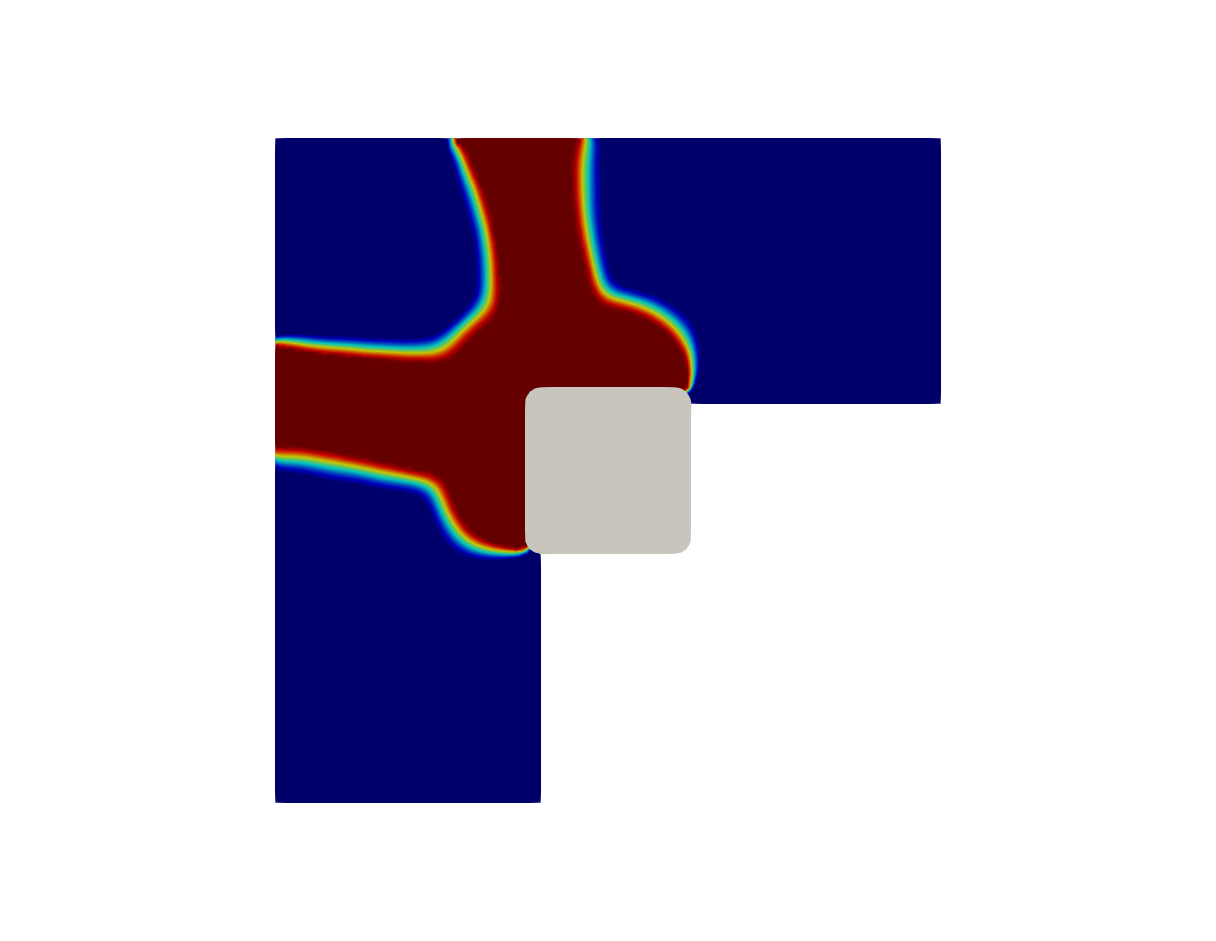
\includegraphics[trim={3.6in 1.8in 3.5in 2.5in},clip,width=0.2\textwidth]{Figures/CC3.png}&
        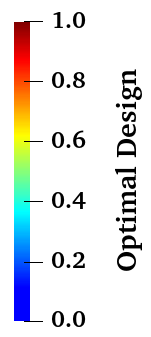
\includegraphics[width=0.06\textwidth]{Figures/design_contour.png}\\
        %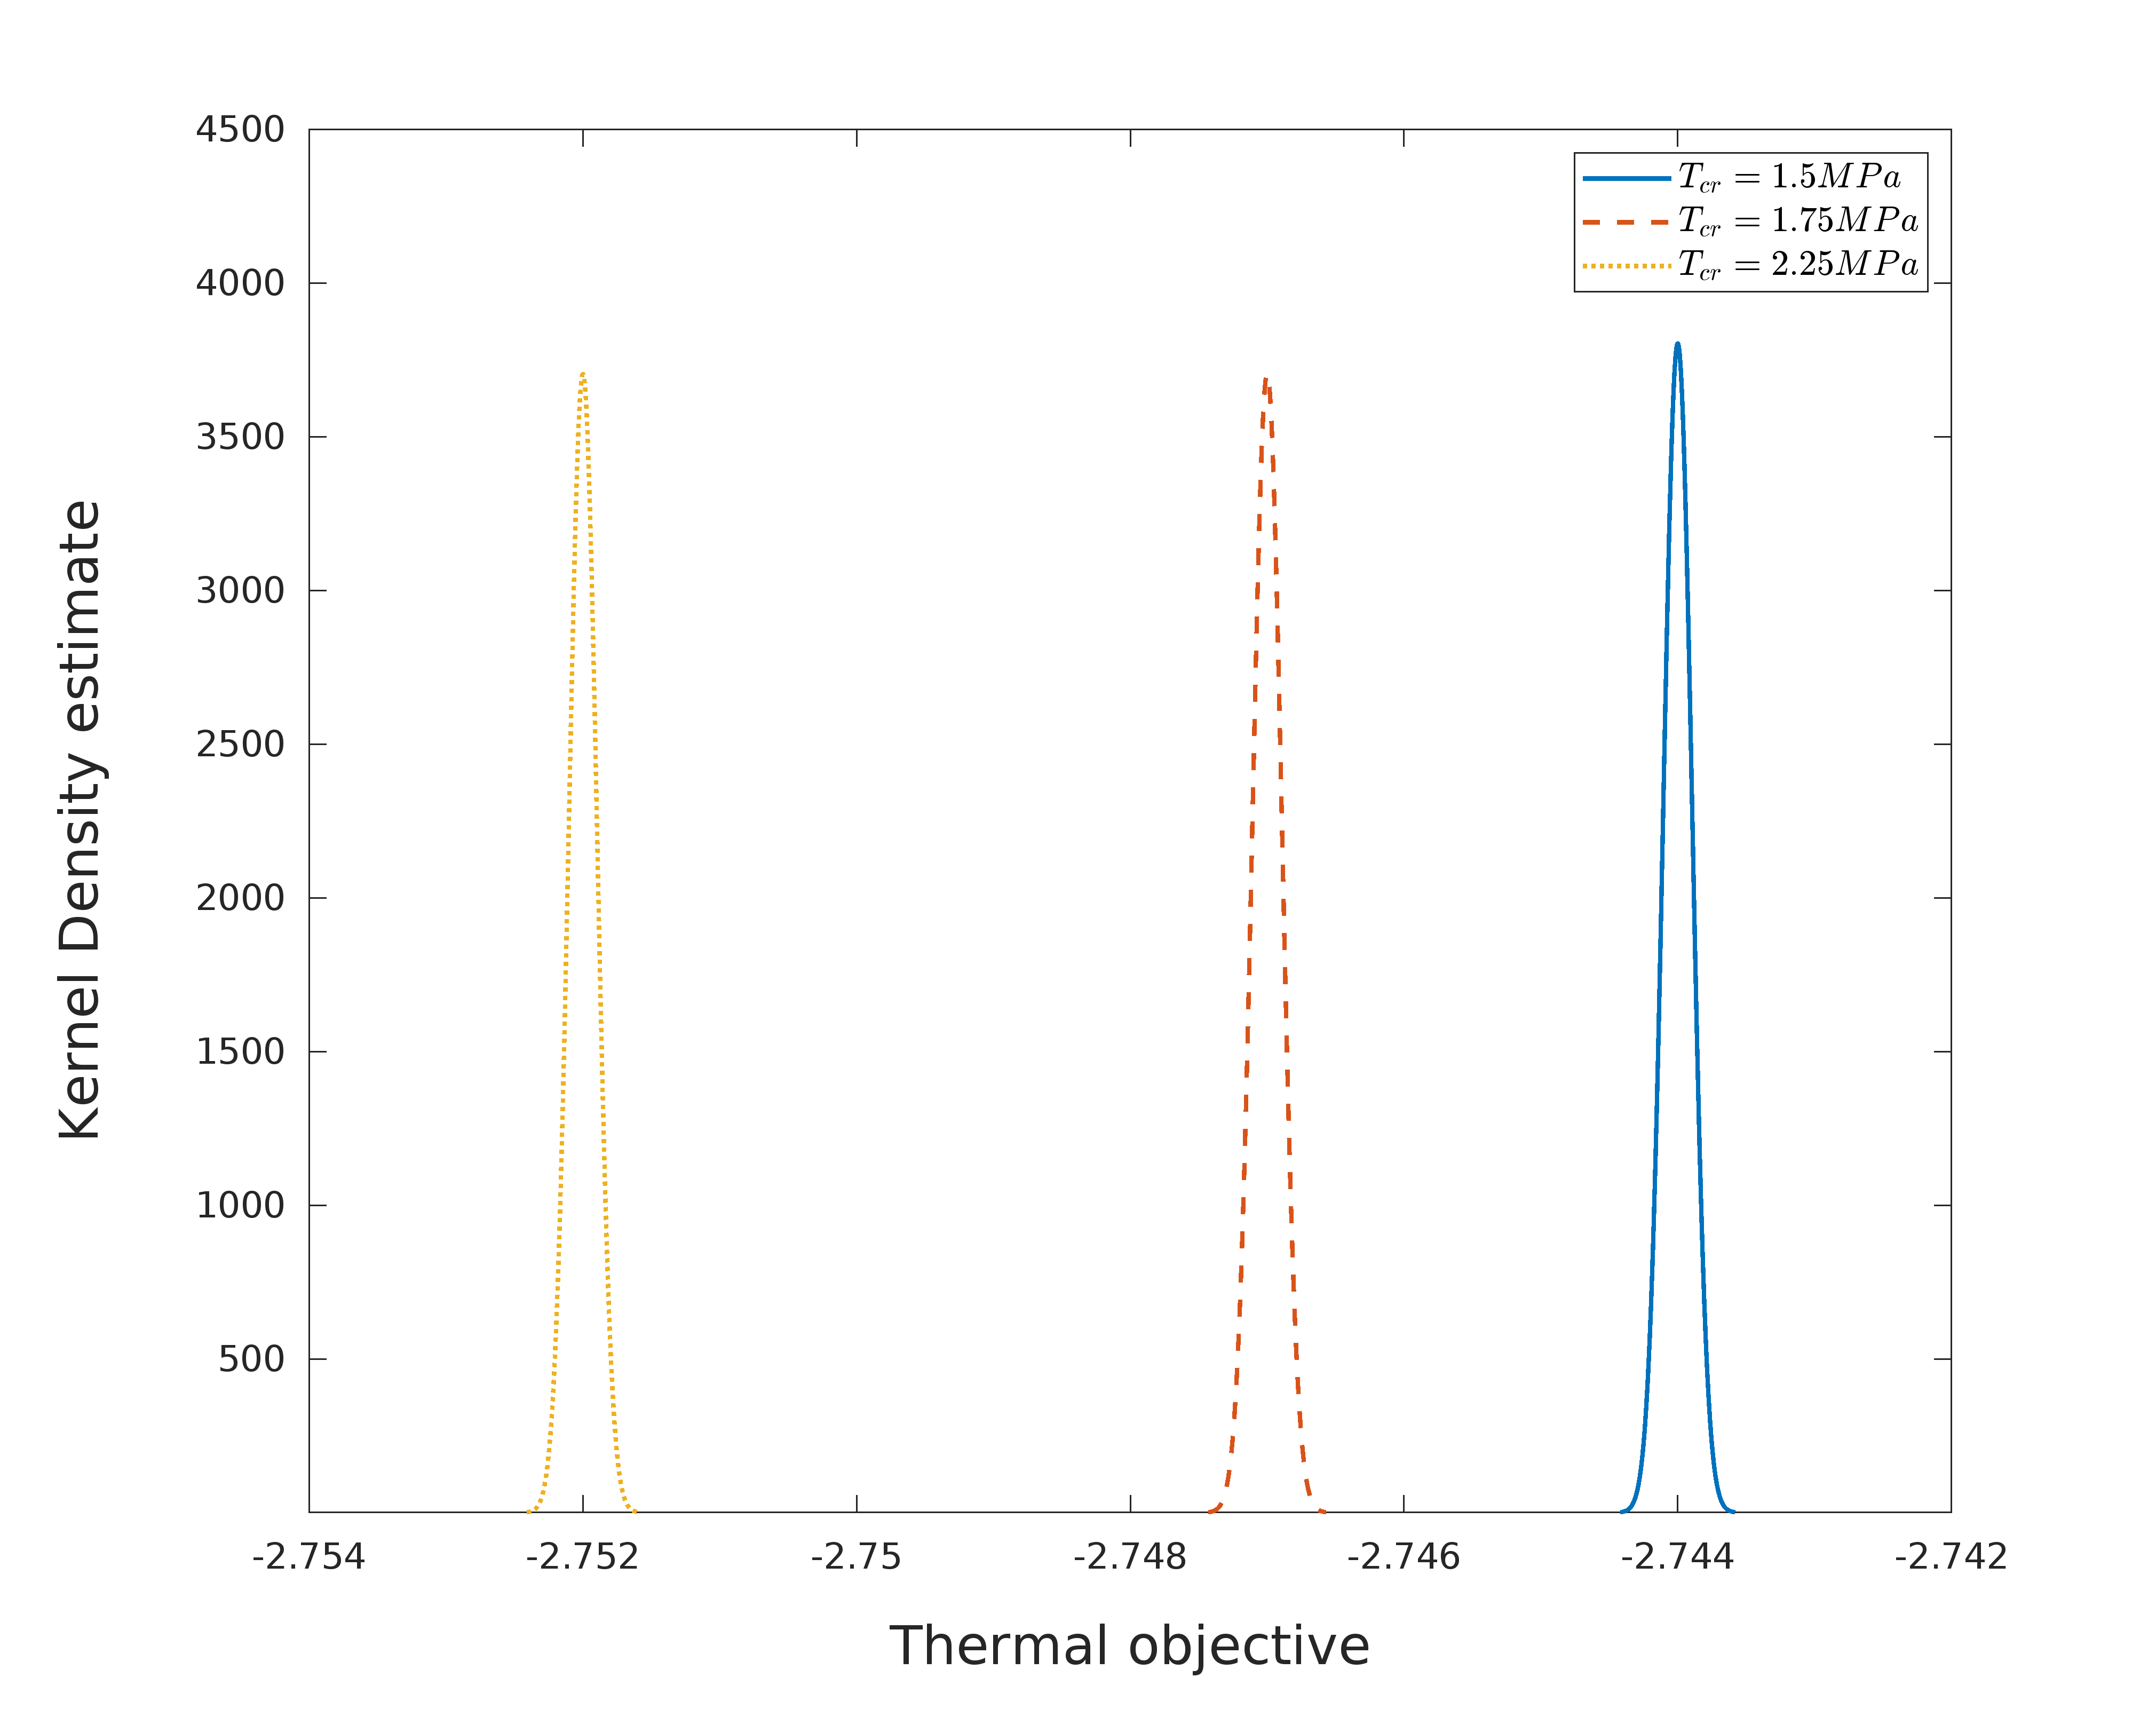
\includegraphics[width=0.4\textwidth]{Figures/CS.png}\\
        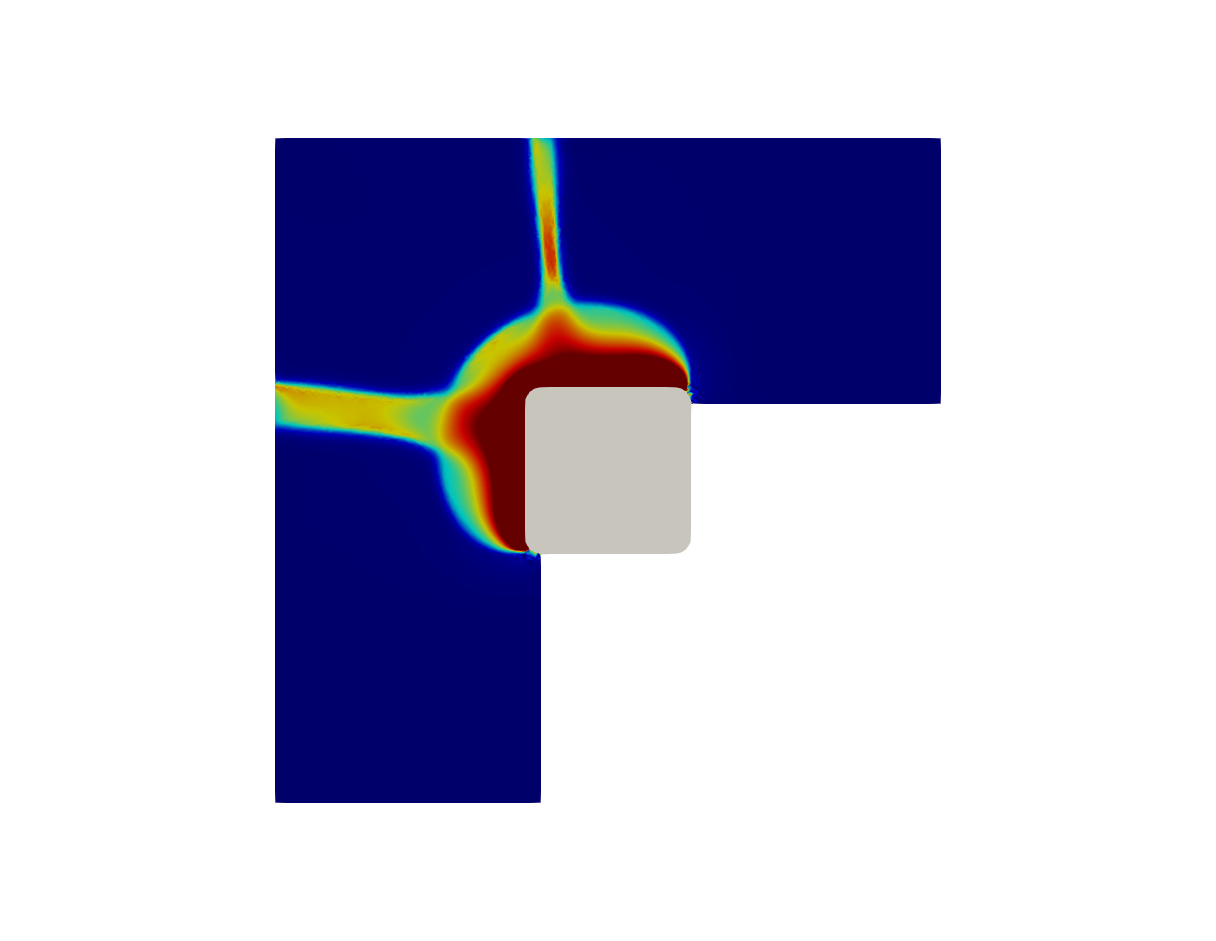
\includegraphics[trim={3.6in 1.8in 3.5in 2.5in},clip,width=0.2\textwidth]{Figures/Stress_CC1.png}&
        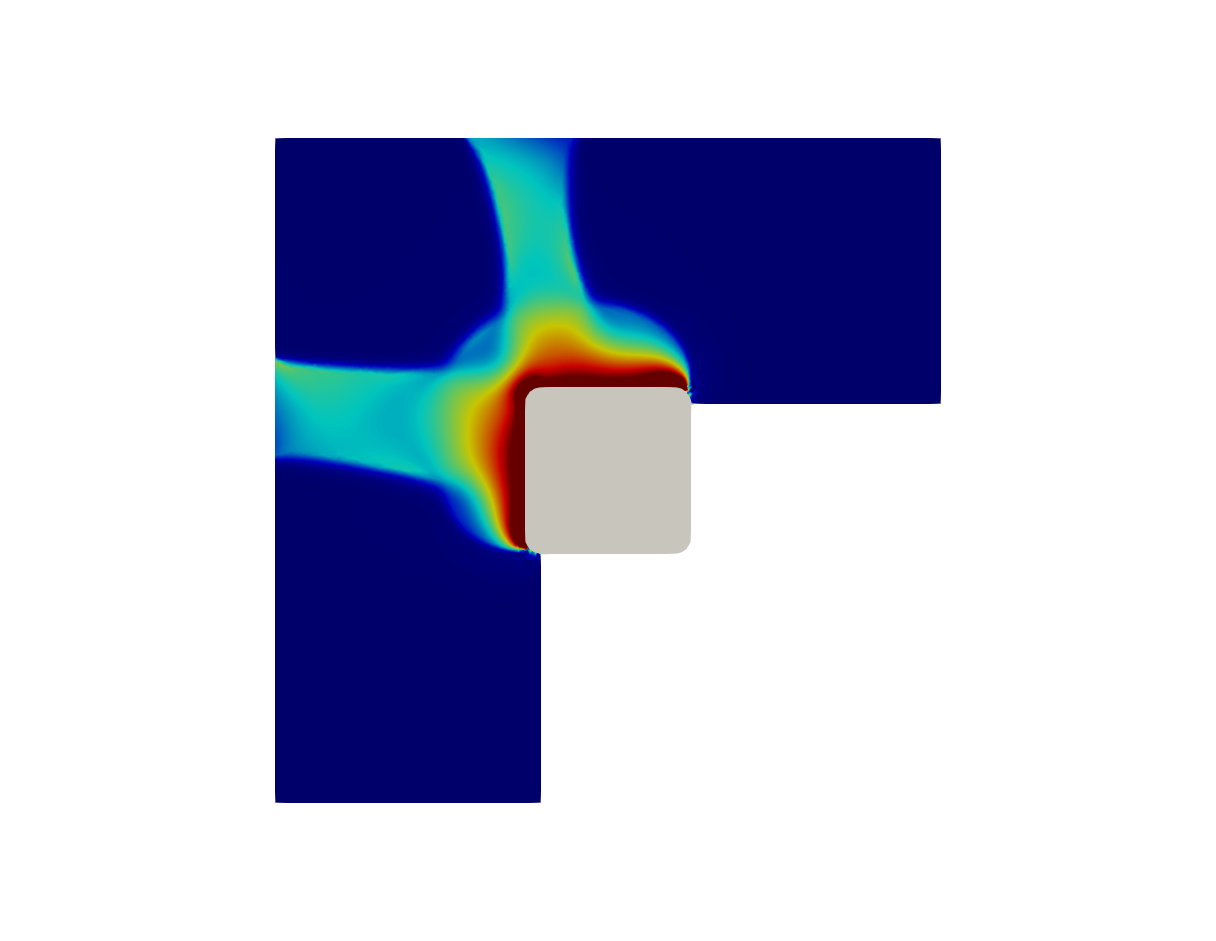
\includegraphics[trim={3.6in 1.8in 3.5in 2.5in},clip,width=0.2\textwidth]{Figures/Stress_CC2.png}&
        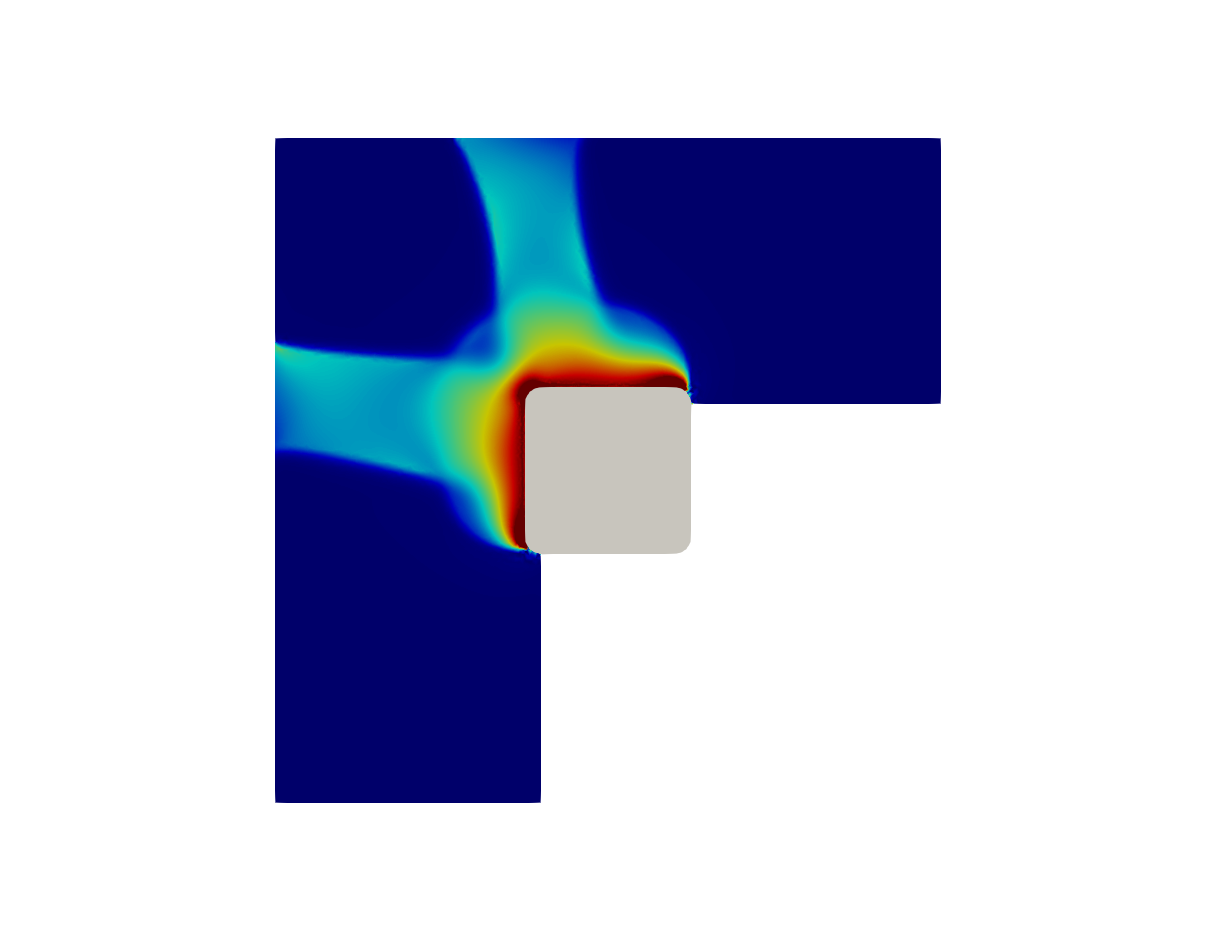
\includegraphics[trim={3.6in 1.8in 3.5in 2.5in},clip,width=0.2\textwidth]{Figures/Stress_CC3.png}&
        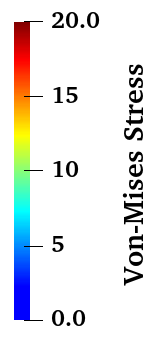
\includegraphics[width=0.06\textwidth]{Figures/CC_contour.png}\\
        $\alpha_{c} = 0.05 $ & $\alpha_{c} = 0.08 $ & $\alpha_{c} = 0.1 $&\\
        \end{tabular}
        
        \label{fig:1}
    \end{figure}
    \fbox{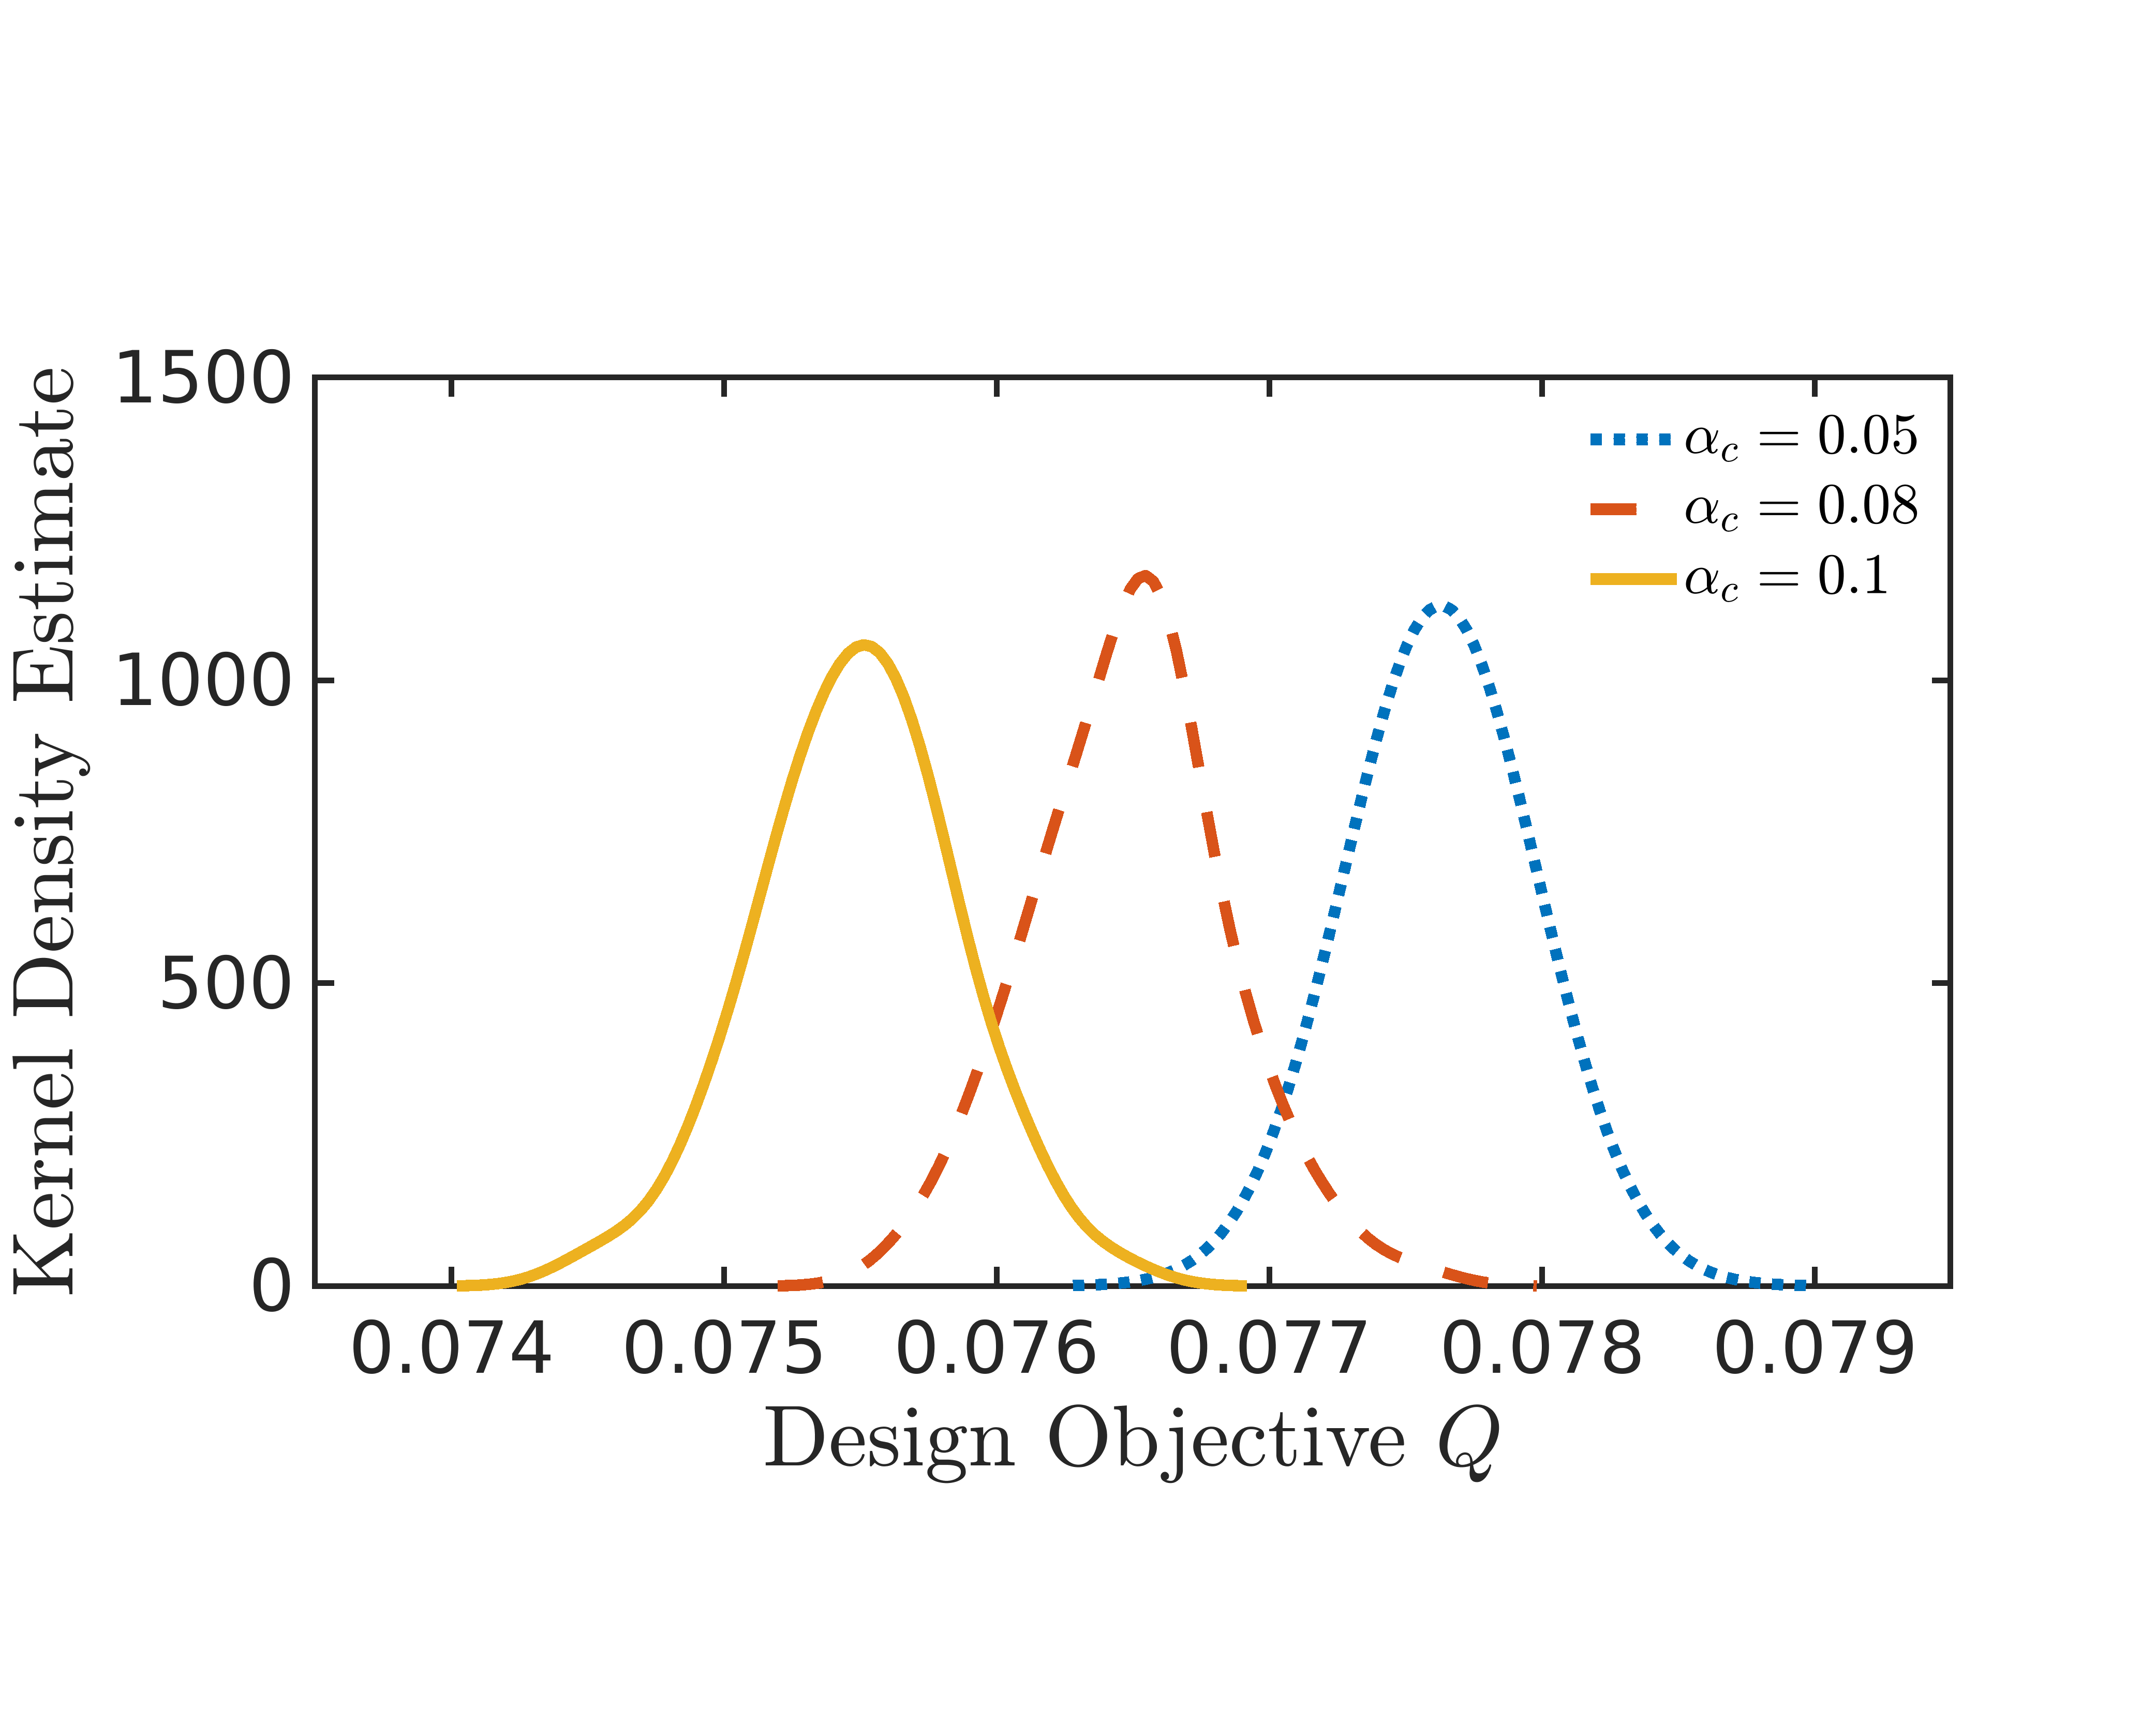
\includegraphics[trim={0in 1in 0in 1.5in},clip,width=0.4\linewidth]{Figures/critical_chance.png}}
    %$\alpha_c = 0.1, \beta_{tik}= 1e-4, \sigma_{\gamma}= 10, \sigma_{\beta}=4, L_c = 0.05, \sigma=0.1, \beta_V =0.1$
\end{frame}


%===================================================

\begin{frame}{Results: State Plots}
\begin{figure}
    \centering
    \begin{tabular}{c c c c}
         Porosity & Displacement & Temperature & Pressure \\
         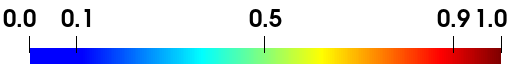
\includegraphics[width=0.18\linewidth]{Figures/porosity_contour.png}&
         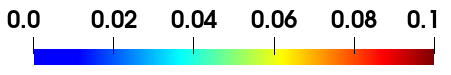
\includegraphics[width=0.18\linewidth]{Figures/Disp_contour.png}&
         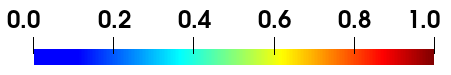
\includegraphics[width=0.18\linewidth]{Figures/temp_contour.png}&
         \includegraphics[width=0.18\linewidth]{Figures/pressure_contour.png}\\
         \hline \vspace{-0.1in}\\
         \includegraphics[trim={3.6in 1.8in 3.5in 2.5in},clip,width=0.18\linewidth]{Figures/porosity.png}&  
         \includegraphics[trim={3.6in 1.8in 3.5in 2.5in},clip,width=0.18\linewidth]{Figures/Disp.png}&
         \includegraphics[trim={3.6in 1.8in 3.5in 2.5in},clip,width=0.18\linewidth]{Figures/Tf.png}&
         \includegraphics[trim={3.6in 1.8in 3.5in 2.5in},clip,width=0.18\linewidth]{Figures/pressure.png}\\
         \hline \vspace{-0.1in}\\
         \includegraphics[trim={3.6in 1.8in 3.5in 2.5in},clip,width=0.18\linewidth]{Figures/porosity_1.png}&  
         \includegraphics[trim={3.6in 1.8in 3.5in 2.5in},clip,width=0.18\linewidth]{Figures/Disp_1.png}&
         \includegraphics[trim={3.6in 1.8in 3.5in 2.5in},clip,width=0.18\linewidth]{Figures/Tf_1.png}&
         \includegraphics[trim={3.6in 1.8in 3.5in 2.5in},clip,width=0.18\linewidth]{Figures/pressure_1.png}\\
         \hline \vspace{-0.1in}\\
         \includegraphics[trim={3.6in 1.8in 3.5in 2.5in},clip,width=0.18\linewidth]{Figures/porosity_2.png}&  
         \includegraphics[trim={3.6in 1.8in 3.5in 2.5in},clip,width=0.18\linewidth]{Figures/Disp_2.png}&
         \includegraphics[trim={3.6in 1.8in 3.5in 2.5in},clip,width=0.18\linewidth]{Figures/Tf_2.png}&
         \includegraphics[trim={3.6in 1.8in 3.5in 2.5in},clip,width=0.18\linewidth]{Figures/pressure_2.png}\\
         \hline \vspace{-0.1in}\\
         
    \end{tabular}
    \label{fig:enter-label}
\end{figure}
\end{frame}
%===============================================================
\begin{frame}{Results: 3D Scenario}
    \begin{figure}
        \centering
        \includegraphics[width=0.52\linewidth]{Figures/3D_F.png}\\
        \footnotesize{Optimal design obtained for a dimension of 100559 design parameters}\\
        \label{fig:enter-label}
    \end{figure}
\end{frame}




%============================================================================================


\section{Conclusions}
\begin{frame}{Outline}
    \tableofcontents[currentsection]
\end{frame}
\begin{frame}{Conclusions}
\small
An efficient framework is introduced for optimal design governed by PDEs including chance constraint under high-dimensional and spatially correlated uncertainty.\vspace{0.05 in}
    \begin{itemize}
        \item Quadratic Taylor approximation for estimating the mean and variance of the design objective with respect to uncertain parameters.
        \vspace{0.05 in}
        \item Chance constraints are implemented using the Von-Mises criterion to avoid \\stress concentration within the beam-insulator system.\vspace{0.05 in}
        \item Efficient trace estimation of the covariance-preconditioned Hessian using a randomized algorithm for solving generalized eigenvalue problems.\vspace{0.05 in}
        \item Control variate is implemented to reduce variance under high uncertainty with the implementation of Monte-Carlo correction.\vspace{0.05 in}
    \end{itemize}
    
\end{frame}

\begin{frame}
    \begin{center}
    \large
    \textbf{Acknowledgement:}\\
        We gratefully acknowledge the support by the U.S. National Science Foundation (NSF) CAREER Award CMMI-2143662\vspace{0.1 in}\\
        \includegraphics[width=0.25\textwidth]{Figures/NSF.png}\\
        \huge{Thank you!}
    \end{center}
\end{frame}




%============================================================================================
%============================================================================================
\end{document}
